% !Mode:: "TeX:UTF-8"
%# -*- coding:utf-8 -*-

%% 南京大学学位论文的示例文档
%% 作者:njuhan: https://github.com/njuHan
%% 源模版repo: https://github.com/njuHan/njuthesis-nju-thesis-template

\documentclass[winfonts,master,twoside]{njuthesis}
\usepackage{tikz}
\usepackage{pgfplots}
%% njuthesis 文档类的可选参数有:
%%   winfonts, linuxfonts, macfonts, adobefonts winfonts 选项使得文档使用Windows 系统提供的字体;linuxfonts 选项使得文档使用Linux 系统提供的字体;macfonts 选项使得文档使用Mac 系统提供的字体;adobefonts 选项使得文档使用Adobe提供的OTF中文字体(需自行下载安转)
%%   phd/master/bachelor 选择博士/硕士/学士论文
%%   twoside 或 oneside 指定排版的文档为双面打印或单面打印格式(twoside会使得chapter 章节从奇数页开始,即纸张的正面开始,因此会出现一些空白的页面)
%%   nobackinfo 取消封二页导师签名信息。注意,按照南大的规定,是需要签名页的。

\lstset{
	columns=fixed,       
	basicstyle=\small,
	numbers=left,                                        % 在左侧显示行号
	numberstyle=\tiny\color{gray},                       % 设定行号格式
	frame=none,                                          % 不显示背景边框
	backgroundcolor=\color[RGB]{245,245,244},            % 设定背景颜色
	keywordstyle=\color[RGB]{40,40,255},                 % 设定关键字颜色
	numberstyle=\footnotesize\color{darkgray},           
	commentstyle=\it\color[RGB]{0,96,96},                % 设置代码注释的格式
	stringstyle=\rmfamily\slshape\color[RGB]{128,0,0},   % 设置字符串格式
	showstringspaces=false,                              % 不显示字符串中的空格
}
\renewcommand{\lstlistingname}{代码}

%%%%%%%%%%%%%%%%%%%%%%%%%%%%%%%%%%%%%%%%%%%%%%%%%%%%%%%%%%%%%%%%%%%%%%%%%%%%%%%
% set up labelformat and labelsep for subfigure 详见: http://www.latexstudio.net/archives/8652.html
\captionsetup[subfigure]{labelformat=simple, labelsep=space}

%%%%%%%%%%%%%%%%%%%%%%%%%%%%%%%%%%%%%%%%%%%%%%%%%%%%%%%%%%%%%%%%%%%%%%%%%%%%%%%
% 设置论文的中文封面

% 单行论文标题,不可换行
\title{模型驱动的IoT服务组合技术研究}

% 如果论文标题过长,可以分两行,第一行用\titlea{}定义,第二行用\titleb{}定义,
% 使用以下3行:
%\title{} %用于覆盖单行标题内容为空
%\titlea{长标题第一行}  %第一行标题写这里
%\titleb{长标题第二行用于长标题换行} %第二行标题写这里
% 注意: \title 不能都注释,它用于控制标题选择双行还是单行。\title{}如果内容为空,则编译\titlea{},titleb{}双行标题,否则编译单行标题


% 论文作者姓名
\author{汤聪}
% 论文作者联系电话
\telphone{-}
% 论文作者电子邮件地址
\email{1195882464@qq.com}
% 论文作者学生证号
\studentnum{MF1933083}
% 论文作者入学年份(年级)
\grade{2019}
% 论文作者毕业年份(届), 出版授权书的学位年度
\graduateyear{2022}
% 导师姓名职称
\supervisor{曹春~~教授}
% 导师的联系电话
\supervisortelphone{}
% 论文作者的学科与专业方向
\major{计算机技术}
% 论文作者的研究方向
\researchfield{软件方法学}
% 论文作者所在院系的中文名称
\department{计算机科学与技术系}
% 论文作者所在学校或机构的名称。此属性可选,默认值为``南京大学''。
\institute{南京大学}
% 论文的提交日期,需设置年、月、日。
\submitdate{2022年 05 月 19 日}
% 论文的答辩日期,需设置年、月、日。
\defenddate{2022年 05 月 19 日}
% 论文的定稿日期,需设置年、月、日。
% 此属性可选,若注释\date{},则默认值为最后一次编译时的日期,精确到日。
\date{2022年 05 月 19 日}

%%%%%%%%%%%%%%%%%%%%%%%%%%%%%%%%%%%%%%%%%%%%%%%%%%%%%%%%%%%%%%%%%%%%%%%%%%%%%%%
% 设置论文的英文封面

% 论文的英文标题,不可换行
\englishtitle{Research on Model Driven IoT Service Composition}
% 论文作者姓名的拼音
\englishauthor{TANG CONG}
% 导师姓名职称的英文
\englishsupervisor{Professor CAO Chun}
% 论文作者学科与专业的英文名
\englishmajor{Computer Technology}
% 论文作者所在院系的英文名称
\englishdepartment{Department of Computer Science and Technology}
% 论文作者所在学校或机构的英文名称。此属性可选,默认值为``Nanjing University''。
\englishinstitute{Nanjing University}
% 论文完成日期的英文形式,它将出现在英文封面下方。需设置年、月、日。日期格式使用美国的日期
% 格式,即``Month day, year'',其中``Month''为月份的英文名全称,首字母大写;``day''为
% 该月中日期的阿拉伯数字表示;``year''为年份的四位阿拉伯数字表示。
% 此属性可选,若注释掉\englishdate{},则默认值为最后一次编译时的日期。
\englishdate{May 19, 2022}

%%%%%%%%%%%%%%%%%%%%%%%%%%%%%%%%%%%%%%%%%%%%%%%%%%%%%%%%%%%%%%%%%%%%%%%%%%%%%%%
% 设置论文的中文摘要

% 设置中文摘要页面的论文标题及副标题的第一行。
% 此属性可选,其默认值为使用|\title|命令所设置的论文标题
\abstracttitlea{模型驱动的IoT服务组合技术研究}
% 设置中文摘要页面的论文标题及副标题的第二行。
% 此属性可选,其默认值为空白
%\abstracttitleb{基于Actor模型的IoT服务组合技术研究}

%%%%%%%%%%%%%%%%%%%%%%%%%%%%%%%%%%%%%%%%%%%%%%%%%%%%%%%%%%%%%%%%%%%%%%%%%%%%%%%
% 设置论文的英文摘要

% 设置英文摘要页面的论文标题及副标题的第一行。
% 此属性可选,其默认值为使用|\englishtitle|命令所设置的论文标题
\englishabstracttitlea{Research on Model Driven IoT Service Composition}
% 设置英文摘要页面的论文标题及副标题的第二行。
% 此属性可选,其默认值为空白
%\englishabstracttitleb{nglishabstracttitleb}

%%%%%%%%%%%%%%%%%%%%%%%%%%%%%%%%%%%%%%%%%%%%%%%%%%%%%%%%%%%%%%%%%%%%%%%%%%%%%%
%% 盲审命令,空白字段设置请看 .cls文件 \newcommand*{\blind}
%% 此外,请按照盲审要求自行去掉个人简历、致谢等页面中的个人信息
%\blind

%%%%%%%%%%%%%%%%%%%%%%%%%%%%%%%%%%%%%%%%%%%%%%%%%%%%%%%%%%%%%%%%%%%%%%%%%%%%%%%
\begin{document}

%%%%%%%%%%%%%%%%%%%%%%%%%%%%%%%%%%%%%%%%%%%%%%%%%%%%%%%%%%%%%%%%%%%%%%%%%%%%%%%

% 制作国家图书馆封面(博士学位论文才需要)
%\makenlctitle
% 制作中文封面
\maketitle
% 制作英文封面
\makeenglishtitle


%%%%%%%%%%%%%%%%%%%%%%%%%%%%%%%%%%%%%%%%%%%%%%%%%%%%%%%%%%%%%%%%%%%%%%%%%%%%%%%
% 开始前言部分
\frontmatter

%%%%%%%%%%%%%%%%%%%%%%%%%%%%%%%%%%%%%%%%%%%%%%%%%%%%%%%%%%%%%%%%%%%%%%%%%%%%%%%
% 论文的中文摘要
\begin{abstract}

随着物联网市场(智能家居,智慧工厂等)不断扩大,IoT设备的种类和数量极速增长,用户倾向于通过场景(一系列IoT服务的命令组合)来操纵IoT服务,而并发的场景运行和服务故障会带来不可逆的后果,这给IoT服务组合系统的开发带来了很大挑战。为了降低IoT服务组合系统的开发难度,并保证并发场景运行的安全性和高效性,研究并实现一套IoT服务组合框架成为必要。针对现有IoT服务组合工作中因缺乏考虑服务组合逻辑建模和缺乏考虑场景并发运行而导致的IoT服务组合系统运行效率低下的问题,本文基于Actor模型构建了IoT服务组合框架。

具体而言,本文的工作主要包括:

\begin{itemize}
    \item 提出了一种基于有限状态机模型和事件驱动模型的IoT服务组合模型:通过有限状态机模型描述IoT服务内部的状态转移逻辑,通过事件驱动模型描述IoT服务之间的交互逻辑。
    \item 给出了一个基于Actor模型的IoT服务组合框架—Cora:用实体关系模型管理IoT服务模型,为IoT服务动态生成统一管理接口;在并发处理中,在保证场景完整性和有序性的前提下,最大程度地减少场景阻塞时间。
    \item 对Cora进行了具体实现,并在真实的智能家居场景中进行实验评估。实验结果表明,Cora具有良好的可用性,能够支持复杂场景的构建和部署;并发测试实验表明,Cora可以支持并发场景,保证场景完整性和有序性,并在与同类系统对比下,具有很好的阻塞延时表现。
\end{itemize}

% 中文关键词。关键词之间用中文全角分号隔开,末尾无标点符号。
\keywords{IoT服务组合框架;模型驱动;Actor模型;接口生成}
\end{abstract}

%%%%%%%%%%%%%%%%%%%%%%%%%%%%%%%%%%%%%%%%%%%%%%%%%%%%%%%%%%%%%%%%%%%%%%%%%%%%%%%
% 论文的英文摘要
\begin{englishabstract}
With the expansion of the smart market(smart home,factories,logistics), the types and number of IoT devices are growing rapidly, making them complex to manage. Nowadays, users prefer to manipulate IoT devices through scenario(a series of IoT service commands), but concurrent scenarios and IoT service failure will bring irreversible consequences, which brings great challenges to the development of IoT service composition system. In order to reduce the development difficulty of IoT service composition system and ensure the safety and efficiency of concurrent scenarios, we present Cora, an IoT service composition framework based on the Actor model.

The primary contributions of this thesis are:
\begin{itemize}
    \item An IoT service composition model based on finite state machine and event driven model is proposed: the state transition logic in IoT service is described by finite state machine model, and the interaction logic between IoT services is described by event driven model.
    \item Cora, the framework of IoT service composition based on the Actor model, is introduced. Cora can generate unified management API for IoT services dynamically; during concurrent scenario, Cora guarantees the integrity and order of the scenario,and presents minimized scenario blocking time.
    \item Implemention of Cora, and an experimental evaluation.Experiment shows that Cora supports the deployment of smart home scenarios. During the concurrent test,Cora ensures the safety of scenarios, and has excellent blocking delay performance compared with similar systems.
\end{itemize}

% 英文关键词。关键词之间用英文半角逗号隔开,末尾无符号。
\englishkeywords{IoT Service Composition; Model Driven; Actor Model; API Generation}

\end{englishabstract}

%%%%%%%%%%%%%%%%%%%%%%%%%%%%%%%%%%%%%%%%%%%%%%%%%%%%%%%%%%%%%%%%%%%%%%%%%%%%%%%
% 生成论文目录
\tableofcontents

%%%%%%%%%%%%%%%%%%%%%%%%%%%%%%%%%%%%%%%%%%%%%%%%%%%%%%%%%%%%%%%%%%%%%%%%%%%%%%%
% 生成插图清单。如无需插图清单则可注释掉下述语句。
\listoffigures

%%%%%%%%%%%%%%%%%%%%%%%%%%%%%%%%%%%%%%%%%%%%%%%%%%%%%%%%%%%%%%%%%%%%%%%%%%%%%%%
% 生成附表清单。如无需附表清单则可注释掉下述语句。
\listoftables

%%%%%%%%%%%%%%%%%%%%%%%%%%%%%%%%%%%%%%%%%%%%%%%%%%%%%%%%%%%%%%%%%%%%%%%%%%%%%%%
% 开始正文部分
\mainmatter

%%%%%%%%%%%%%%%%%%%%%%%%%%%%%%%%%%%%%%%%%%%%%%%%%%%%%%%%%%%%%%%%%%%%%%%%%%%%%%%
% 学位论文的正文应以《绪论》作为第一章
\chapter{绪论}\label{chapter_introduction}
\section{研究背景}
物联网(The Internet of Things)\cite{iot}是基于互联网、广播电视网、传统电信网等信息承载体,让所有能够被独立寻址的普通物理对象实现互联互通的网络。物联网被认为是信息科学技术产业的第三次革命,如今,物联网连接数实现爆发式增长,根据相关研究数据\cite{smarthometrend}显示:截至2020年底,全球物联网市场规模2480亿美元,较上年增加360亿美元,同比增长17\%;全球物联网设备数量126亿个,较上年增加19亿个,同比增长17.76\%;其中交通物流、工程制造、智慧城市和智能家居是物联网的主要发展方向,“万物物联”成为全球网络未来发展的重要方向。


IoT设备是物联网的基础,IoT设备\cite{broring2011new}是指能够通过网络通讯协议传输数据的非标准计算设备。IoT设备是异构的,几乎没有标准的描述,IoT设备的异构性会对IoT设备的管理造成困难\cite{atzori2010internet},将物理的IoT设备在信息空间中映射为IoT服务\cite{huang2016service}可以消解这种异构性,用户可以在IoT设备管理平台中调用IoT服务完成对IoT设备的控制。而对多个IoT服务进行组合可以实现更加复杂的需求,扩展IoT的应用场景\cite{asghari2018service}。例如在智慧物流中\cite{hamzei2018toward},可以将智能机器人检索货物、包装货物、给货物贴上地址标签等IoT服务进行组合,构建完整的智慧出货流程,这样不仅可以提高出货效率,还能降低出错概率。

然而当前的IoT服务组合技术很难满足开发人员的开发需求,同时可能影响用户体验,面临着诸多挑战。以智能家居场景为例:一方面,设备数量和种类的增加带来了开发适配和维护的负担\cite{brush2011home},预计到2023年,平均每户将拥有超过30个智能家居设备\cite{alam2012review};另一方面,用户的需求也正在变得更加复杂,用户期望将智能家居当做一个整体来管理,而不是一堆独立的设备\cite{mennicken2012hacking}。但是随着IoT服务组合场景应用越来越广泛,设备故障和场景运行中的错误会极大地影响用户体验。例如假设用户定义了打开空调之后自动关闭客厅的门窗的流程,但是如果空调打开后,门窗无法自动关闭,则会执行失败,影响用户体验。

本文将IoT服务组合实例称为\textbf{场景}\cite{DBLP:journals/fgcs/ArellanesL20},两个典型的场景如下:

\begin{quote}
\textit{洗衣服场景}:\{\emph{洗衣机打开;洗衣机运行30分钟;洗衣机关闭;烘干机打开;烘干机运行20分钟;烘干机关闭}\}。

\textit{净化空气场景}:\{\emph{窗户关闭;净化器打开;净化器运行}\}。
\end{quote}

对于开发人员来说,场景构建具有如下挑战:

\textbf{IoT服务交互}:在智慧城市、智能工厂等应用场景中,由不同IoT设备厂商和代理商拥有和管理的物联网服务被大规模部署是非常常见的。但是由于IoT设备厂商之间存在不可忽视的技术壁垒,不同设备厂商提供的IoT服务构建流程及管理接口也存在较大差异,例如小米IoT开发者平台\cite{xiaomiiot}和华为IoT物联网社区\cite{huaweiiot}提供了不同的开发流程和服务接口设计规范。在这种情况下,对开发人员来说,了解这些不同的IoT服务的接口以及基于这些接口管理、查询和交换IoT服务的信息,进而实现场景构建不仅需要消耗大量的时间和精力,还存在着巨大的错误风险。因此为不同厂商的IoT服务构建标准统一的管理接口,可以降低开发人员进行场景构建的学习成本和错误风险。

\textbf{领域知识门槛}:物联网应用开发的领域知识门槛会给开发人员带来很大的学习成本。尽管IoT设备的服务化可以降低一定的开发门槛,但是开发人员为了使用和集成单一物联网服务而需要了解的内部细节和操作的数量也是不可忽视的。因此为了降低领域知识门槛,可以基于模型驱动开发来进行IoT服务组合框架构建。


而对于用户来说,场景运行需要保证如下特性:

\textbf{场景完整性}:场景完整性要求运行中的场景不能被打断或终止,换言之,当场景一旦开始执行,则需要执行结束\cite{zave2015toward}。例如当用户运行\textit{净化空气场景}时,如果净化器出现故障或者整个场景执行过程被意外终止,那么\textit{净化空气场景}就会执行失败,场景中IoT服务所处的状态也是用户无法接受的——窗户打开,净化器运行(浪费能源)或者窗户关闭,净化器关闭(空气变差)。因此在场景运行时,IoT服务组合平台需要保证场景完整性。

\textbf{场景有序性}:场景有序性要求并发运行场景时,需要保证IoT服务执行不同场景的指令之间相对有序\cite{leesatapornwongsa2020transactuations}。因为IoT服务串行执行所有指令,所以冲突问题产生的原因是:不同场景执行时发送给同一IoT服务执行指令,而执行指令之间存在相反的运行逻辑。
例如当净化器服务在执行完净化器打开指令之后,接收并执行并发场景中净化器关闭指令,最后净化器服务接收到净化器运行指令,但是净化器服务无法在关闭状态下执行运行指令,造成场景执行错误。因此为了避免场景执行错误,在场景并发运行中,IoT服务组合平台需要保证场景有序性。 

\textbf{场景高效性}:场景高效性要求并发运行场景时,需要在保证场景完整性和场景有序性的前提下,减少场景阻塞时间。例如用户A和用户B同时运行\textit{洗衣服场景}时,在保证场景完整性和有序性的前提下,最坏情况下两个场景需要依次执行,则阻塞的用户需要等待50分钟,而最优情况下,洗衣机服务在完整执行完一个场景的任务后,可以立即执行第二个场景的任务,则阻塞的用户只需等待30分钟,因此场景高效性能够影响用户体验,IoT服务组合平台应尽可能减少场景阻塞时间。

% 本文认为上述挑战的关键在于忽略了IoT设备的物理特性,将IoT服务与web服务混淆看待。但是IoT服务与web服务不同在于,IoT服务依托于IoT设备,是IoT设备在信息空间中的虚拟映射,需要继承IoT设备的物理特性,例如大部分IoT设备可以认为是独占模式的(单次只能处理一条指令,并发处理指令会造成指令丢失)。

综上,高效的IoT服务组合技术一方面可以降低开发人员的开发负担,提升开发效率;另一方面可以在保证IoT服务组合场景的完整性和有序性的前提下,减少场景阻塞时间,提升用户体验。因此IoT服务组合技术具有重要的研究价值。

\section{研究现状}\label{subsec:mptcp_conges}
目前,伴随着物联网浪潮,“人-机-物”三元融合的智慧应用也越来越普遍,基于IoT服务的IoT设备自动化运行引起了广泛关注,因此IoT服务组合技术近年来在软件工程中成为一个比较热门的研究领域。

首先在工业界,目前对IoT服务组合的技术支持处于起步阶段,对于IoT服务组合场景可能产生的问题关注有限。以智能家居场景为例,一些开源的智能家居设备管理平台如HomeAssistant\cite{homeassistant},OpenHub\cite{soldatos2015openiot}取得了很大的关注,但是这些智能家居设备管理平台主要面向用户,致力于适配各个厂商的种类繁杂的IoT设备,力求为用户提供开箱即用的设备管理服务,但是对于IoT服务组合场景的实践大都处于起步阶段。相较于开源平台,各大厂商的IoT设备管理平台如Google Home,米家等,能够支持IoT服务组合的功能,但是基本采用一种“尽最大努力交付”的策略来执行IoT服务组合场景,对于场景完整性和高效性的支持有限。

在学术界,在IoT服务组合建模领域,Ruowei Xiao\cite{xiao2019finite}等人提出了有限状态机模型驱动的服务组合方法,但对于服务组合的业务逻辑缺乏完整的模型定义;Bo Cheng\cite{cheng2016situation}等人关注于IoT设备属性对IoT服务组合的研究,但是没有关注设备属性可能带来的并发错误。而在冲突处理领域,Shegufta B. Ahsan\cite{ahsan2021home}等人认为IoT服务组合场景具有原子性,并构建了四种可见性模型,但是其原子性定义上值得商榷,并且没有提供框架实现;Dipankar Chaki\cite{chaki2020conflict}等人基于用户历史活动数据,通过深度学习的方式构建用户行为模型,预先进行冲突检测来实现冲突避免,本文认为这种方式过于复杂,预测正确性很难保证。

综上,IoT服务组合的场景建模方法并不完善,对于场景执行的完整性和并发场景运行中的有序性和高效性问题缺乏深入考虑及合理解决方案,并且缺乏完善的IoT服务组合框架支持。


\section{本文主要工作}
本文提出了一套IoT服务组合建模方法及IoT服务组合框架—Cora,开发人员可以基于IoT服务组合模型完成场景构建,而Cora能够在并发场景运行中保证场景完整性、有序性和高效性。针对IoT服务组合场景构建中存在的IoT服务访问接口异构和并发冲突处理等问题,本文基于模型驱动开发方法,从场景建模和框架实现两个层面考虑。首先从场景建模层面看,基于关注点分离(Separation of Concerns,简称SoC)原则,本文将IoT服务的设备属性、IoT服务的内在状态转移逻辑、IoT服务之间的组合逻辑这三个方面充分解耦,提出一套完整的IoT服务组合建模方法,降低开发人员进行场景建模的复杂度;在框架实现层面,框架基于Actor模型构建运行时系统,统一管理IoT服务模型,为IoT服务生成标准统一的IoT服务生命周期管理接口,构建IoT服务的内在状态转移管理引擎,用消息驱动的方式支撑IoT服务之间的交互,框架层在保证场景完整性和有序性的前提下,最大程度地减少场景阻塞时间。

本文提出的智能家居场景下的IoT服务组合框架架构如图1-1所示,自底向上来看:首先将IoT设备服务化,将具体的IoT设备映射到信息空间中的IoT服务,为IoT服务构建设备属性模型;然后为了描述IoT服务的状态转移逻辑,用有限状态机为IoT服务构建状态转移模型;接着通过IoT服务组合模型构建IoT服务组合场景,Cora保证场景的完整性、有序性和高效性;最后,Cora会为IoT服务和场景提供标准统一的管理接口。

综上,本文的研究内容主要包括:
\begin{itemize}
    \item 提出了一种基于有限状态机模型和事件驱动模型的IoT服务组合模型,自底向上地为IoT服务组合建模。通过有限状态机模型描述IoT服务内部的状态转移逻辑,并基于事件驱动模型构建IoT服务之间的交互逻辑。
    \item 给出了一个基于Actor模型的IoT服务组合框架—Cora:用实体关系模型管理IoT服务模型,为IoT服务实例动态生成统一管理接口;基于Actor模型构建框架,在并发处理中,在保证场景完整性和有序性的前提下,最大程度地减少了场景阻塞时间。
    \item 设计实现了Cora,并在真实的智能家居场景中进行实验评估。实验结果表明,IoT服务组合框架Cora具有良好的可用性,能够支持复杂场景的构建和部署,在并发测试实验中,Cora可以支持并发场景,保证了场景完整性和有序性。并在与同类型系统对比下,具有较优的场景阻塞延时表现。
\end{itemize}

\begin{figure}
	\centering
	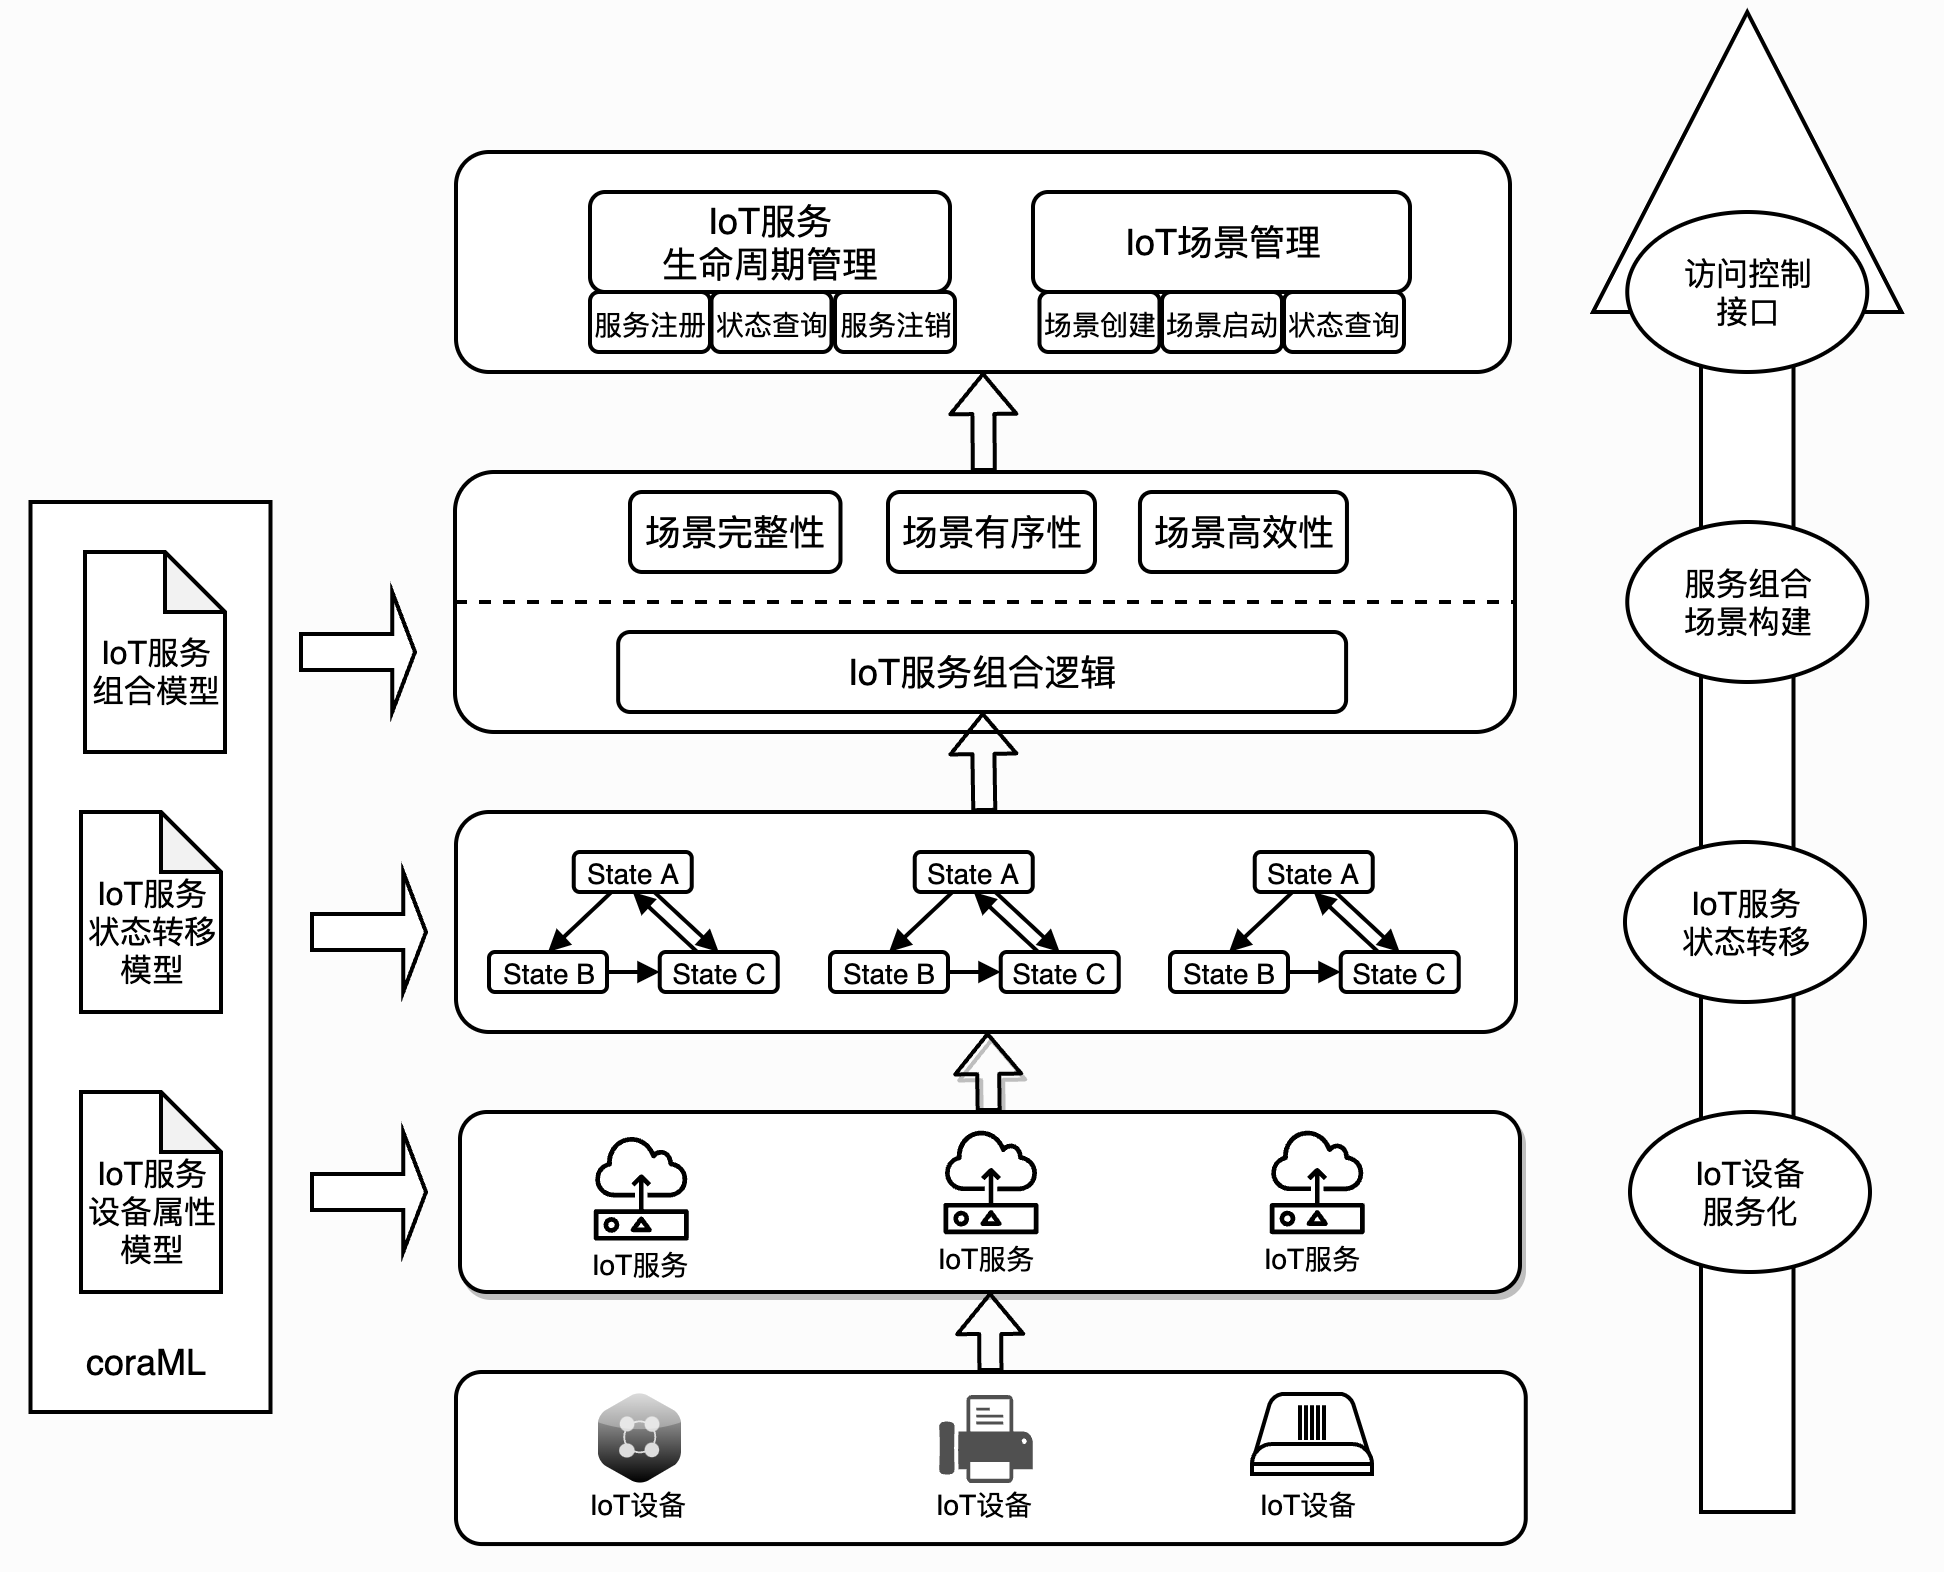
\includegraphics[width=\textwidth]{figure/cora.png}
	\caption{IoT服务组合框架架构}
	\label{overview}
\end{figure}

\section{本文组织结构}

本文组织如下:

第二章介绍了本文涉及到的相关工作。主要包括工业界的IoT服务组合管理平台(开源社区和厂商),IoT服务组合场景建模,IoT服务组合冲突处理和IoT服务组合冲突检测方面的工作。

第三章详细介绍了模型驱动的IoT服务组合建模方法。主要分为IoT服务建模和IoT服务组合逻辑建模两部分。首先介绍了模型驱动开发的相关概念,接着介绍基于IoT服务组合场景本文设计实现的领域特定语言—coraML,然后本文将IoT服务建模拆分为IoT服务设备属性建模和IoT服务状态转移建模两部分分别展开阐述,最后介绍了IoT服务组合建模方法。

第四章详细介绍了基于Actor模型实现的IoT服务组合框架—Cora。主要分为三部分:首先介绍了IoT服务模型管理模块的实现,接着介绍了IoT服务生命周期管理模块的设计,最后阐述了IoT服务组合场景的构建流程。

第五章是实验评估部分,基于真实场景,主要对本文提出的IoT服务组合建模方法和IoT服务组合框架Cora进行了详细的实验评估,验证了本文工作的有效性。

第六章是总结与展望,对本文工作进行简单的总结,并对未来可能的研究方向进行展望。

\chapter{相关工作}
随着物联网的推广应用,IoT服务组合技术近年来在软件工程中成为一个热门的研究领域。本文主要关注IoT服务组合建模方法、基于IoT设备特性的IoT服务组合技术、IoT服务组合中的冲突处理以及IoT服务组合中的冲突检测这四类工作。此外,作为偏实际应用的研究领域,现有的系统也在本文的调研范围中,在开源社区和工业界,有一些优秀的平台和系统也支持了IoT服务组合。下文将从这些领域中选择几个具有代表性的工作,阐述他们的研究内容以及局限性。

\section{IoT服务管理平台}
在工业界,目前IoT设备管理平台实现主要关注于IoT服务的注册连接管理,在IoT服务组合方面的工作并不充分\cite{aoudia2019service}。在开源社区中,主要有HomeAssistant\cite{homeassistant},OpenIoT\cite{soldatos2015openiot},ThingsBoard\cite{thingsboard},PubNub\cite{arunarduino}等项目实现,HomeAssistant是最具代表性的IoT设备管理平台,主要面向智能家居,由Python实现,在github中有超过50k的star数。首先从定位来说,HomeAssistant这类的IoT设备管理平台主要面向用户,致力于为用户提供开箱即用的设备管理服务,所以对于开发人员来说,这些平台的适配能力和复用性存在不足,并且平台的扩展性也存在限制。在服务组合方面,HomeAssistant提供了Automation Condition的概念,本质上是一种基于规则的服务组合方式,用户可以事先声明action,trigger等参数来组合服务,但是在
本文关注的冲突处理和错误处理方面,主要采用“尽最大努力交付”\cite{besteffort}的策略,无法保证场景有序性和高效性。

而在商业平台方面,例如Google Home\cite{googlehome},米家\cite{homemi}等,也主要采用了这种“尽最大努力交付”的策略,无法保证场景有序性和高效性\cite{celik2018soteria}。图2-1展示了Google Home和米家中的场景构建过程,以Google Home为例,用户构建一个Routine时,需要选择该Routine中需要使用的设备并规定设备唤醒时间,但是Routine构建时没有考虑可能存在的设备并发访问情况(在同一时间,家中的不同用户使用同一设备),因此相关数据显示,Google Home在并发场景中存在直接丢弃用户指令的情况\cite{notworking},并且也存在场景无法正常执行完毕的错误发生\cite{error}。
\begin{figure}[H]
	\begin{subfigure}{.5\textwidth}
		\centering
		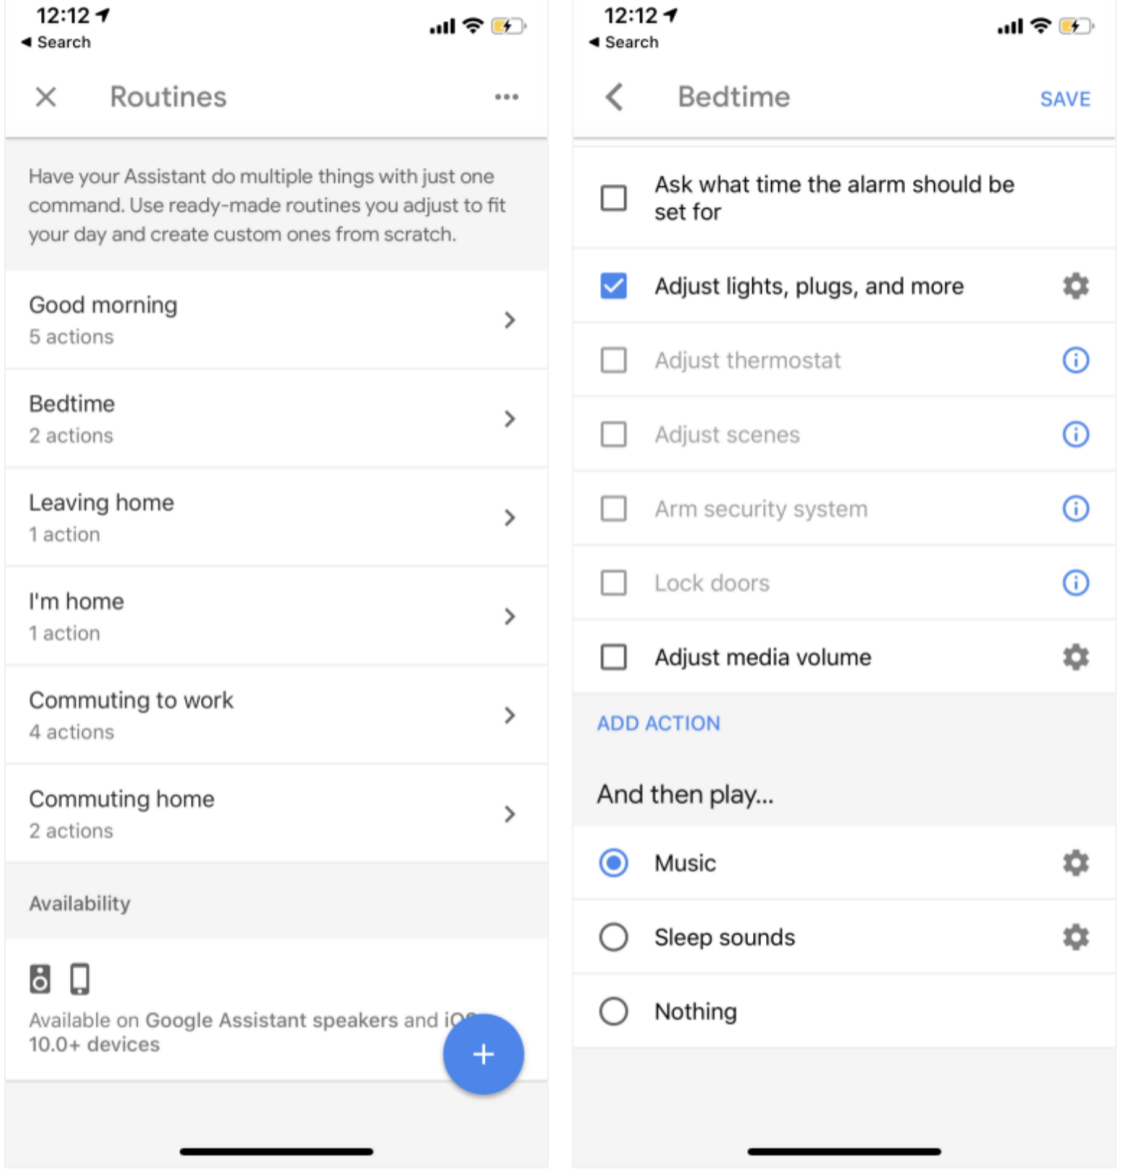
\includegraphics[width=1\textwidth]{figure/2-relatework/google-home-routines.png}
		\caption{Google Home中的场景}
		\label{subfig:a}
	\end{subfigure}
	\begin{subfigure}{.5\textwidth}
		\centering
		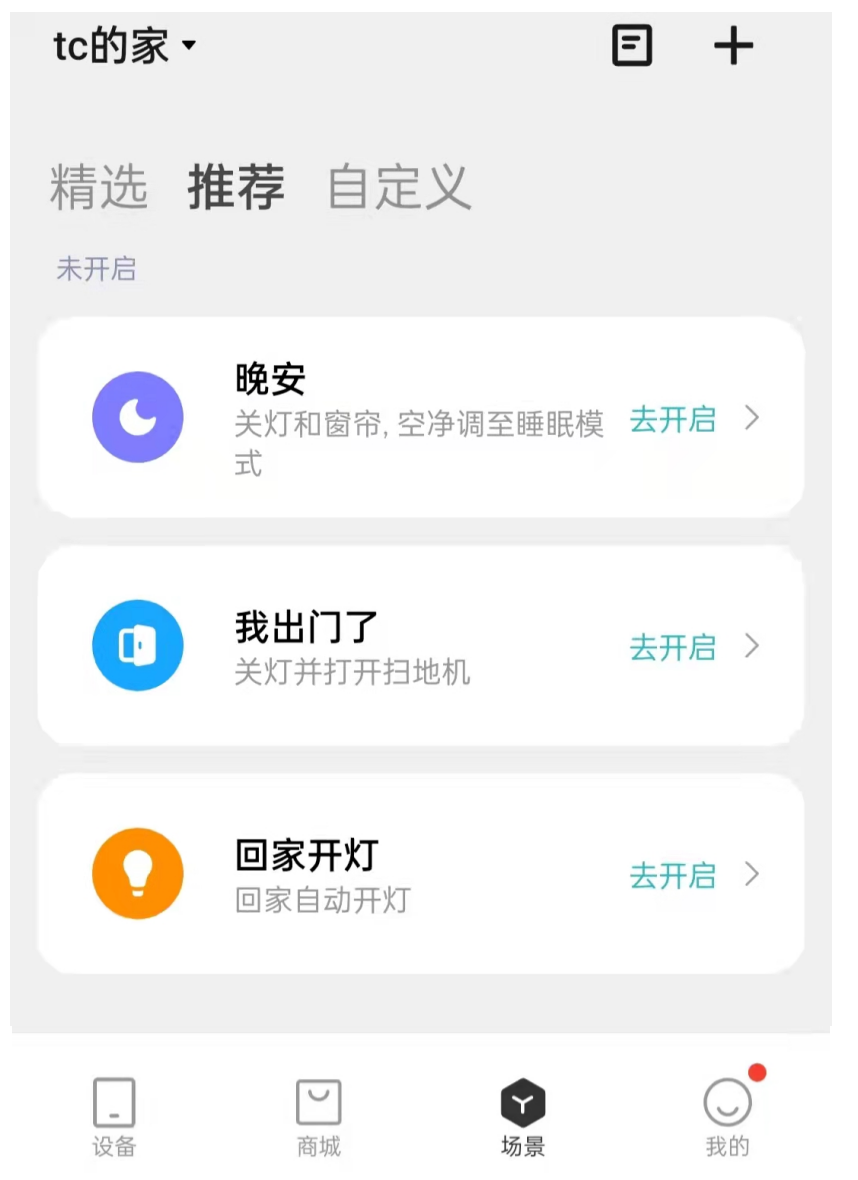
\includegraphics[width=0.8\textwidth]{figure/2-relatework/mihome-context.png}
		\caption{米家中的场景}
		\label{subfig:b}
	\end{subfigure}
\caption{工业界的场景构建实例}
\label{fig:sub}
\end{figure}
\section{IoT服务组合模型}
在IoT服务组合建模方面,Ruowei Xiao等人\cite{xiao2019finite}\cite{tao2018multi}提出了一种模型驱动的服务组合方法,并期望基于该方法快速构建IoT系统原型。其主要工作是提出了用有限状态机模型来为IoT服务的内部运行逻辑建模,并实现了一种领域建模语言—HSML,用模型驱动的方式来为IoT服务的内部运行逻辑建模并提供统一的管理接口,但是其建模方法仅限于对IoT服务建模,没有深入到IoT服务之间的交互逻辑,缺乏对IoT服务间的交互逻辑建模。如图2-2所示,传感器和智能窗帘之间的组合逻辑通过\textit{用户定义的逻辑服务}实现,即通过用户代码实现的方式来完成IoT服务之间的交互。这种建模方式缺乏对IoT服务组合逻辑的建模过程,而这部分建模缺失在实际运行过程中会因为设备故障,并发冲突等带来不必要的错误。
\begin{figure}
	\centering
	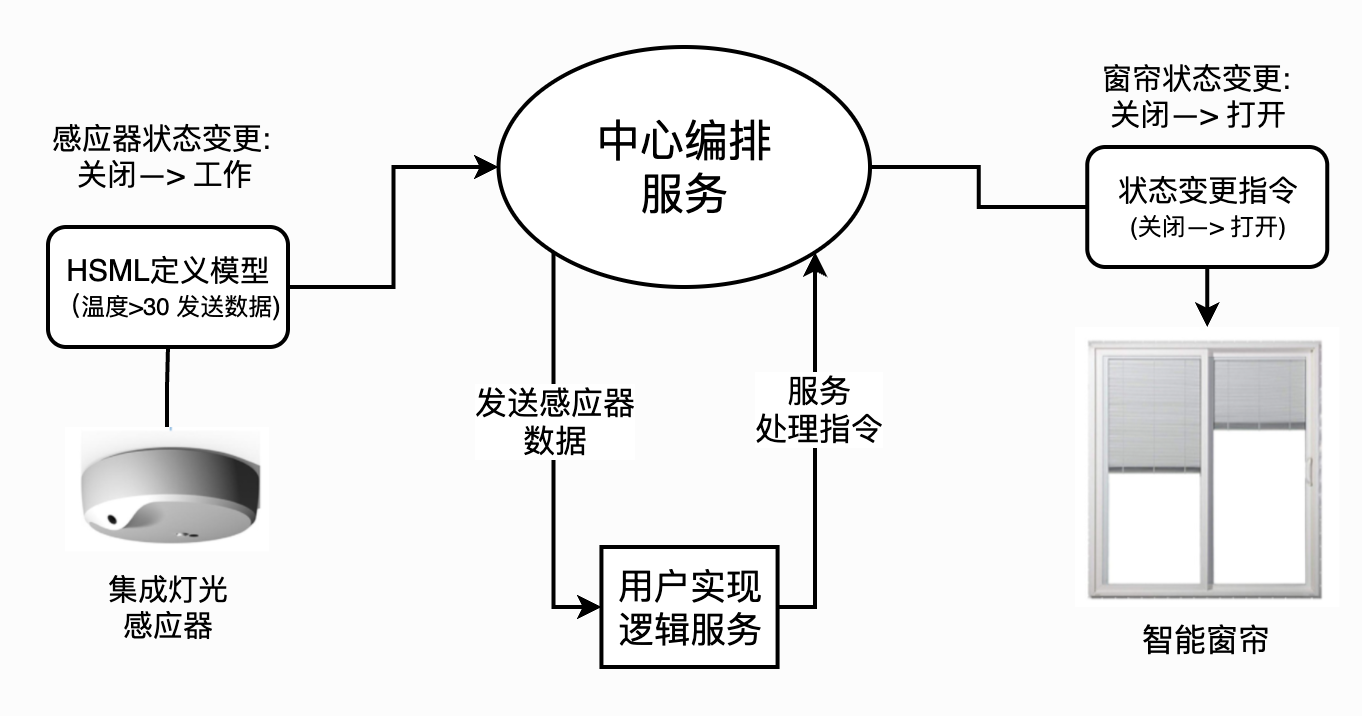
\includegraphics[width=1.0\textwidth]{figure/2-relatework/hsml.png}
	\caption{Ruowei Xiao等人提出的服务组合方法示例}
	\label{ontransact-impl}
\end{figure}

在基于IoT设备特性的IoT服务组合研究方面,Bo Cheng等人\cite{cheng2016situation}\cite{cheng2017situation}\cite{cheng2018lightweight}关注于IoT设备特有的物理属性和时空约束对IoT服务组合的研究。因为与传统web服务不同,IoT服务可以看做IoT设备在网络空间中的一种虚拟映射,所以IoT服务也需要考虑IoT设备的物理属性(是否运行,是否损坏)和时空约束(所处位置,运行时间周期)等,所以考虑物理属性和时空约束的IoT服务组合在真实场景(智慧停车,智慧物流)中具有重大意义。Bo Cheng等人在这方面的模型构建和框架构建方面进行了一系列研究,但是缺乏关注服务组合实例在运行过程中可能出现的问题,并且没有给出一个可以运行的框架,当然这系列工作也给本文带来了很多思考和启发。



\section{IoT服务组合冲突处理}
在IoT服务组合的冲突处理方面, Shegufta B. Ahsan等人\cite{ahsan2021home}\cite{ahsan2019home}提出了SafeHome,给本文的工作带来了很大的启发。SafeHome是IoT服务组合冲突处理领域的首篇工作,该工作聚焦于智能家居的服务组合中的并发问题,首先定义routine(一系列操控IoT服务的指令列表)具有原子性,并在此前提下,针对并发控制,基于锁机制为开发人员提供了四种可见性模型和相关的冲突处理策略,并在多个实际场景中比较了四种模型的适用性,图2-3展示了5个示例场景并发执行时,Safehome中的四种可见性模型示例。场景1和场景2是咖啡机和面包机顺序运行,场景3为面包机运行,场景4为打扫客厅场景,需要扫地机和拖布顺序运行,场景5为清理厨房场景。
\begin{figure}
	\centering
	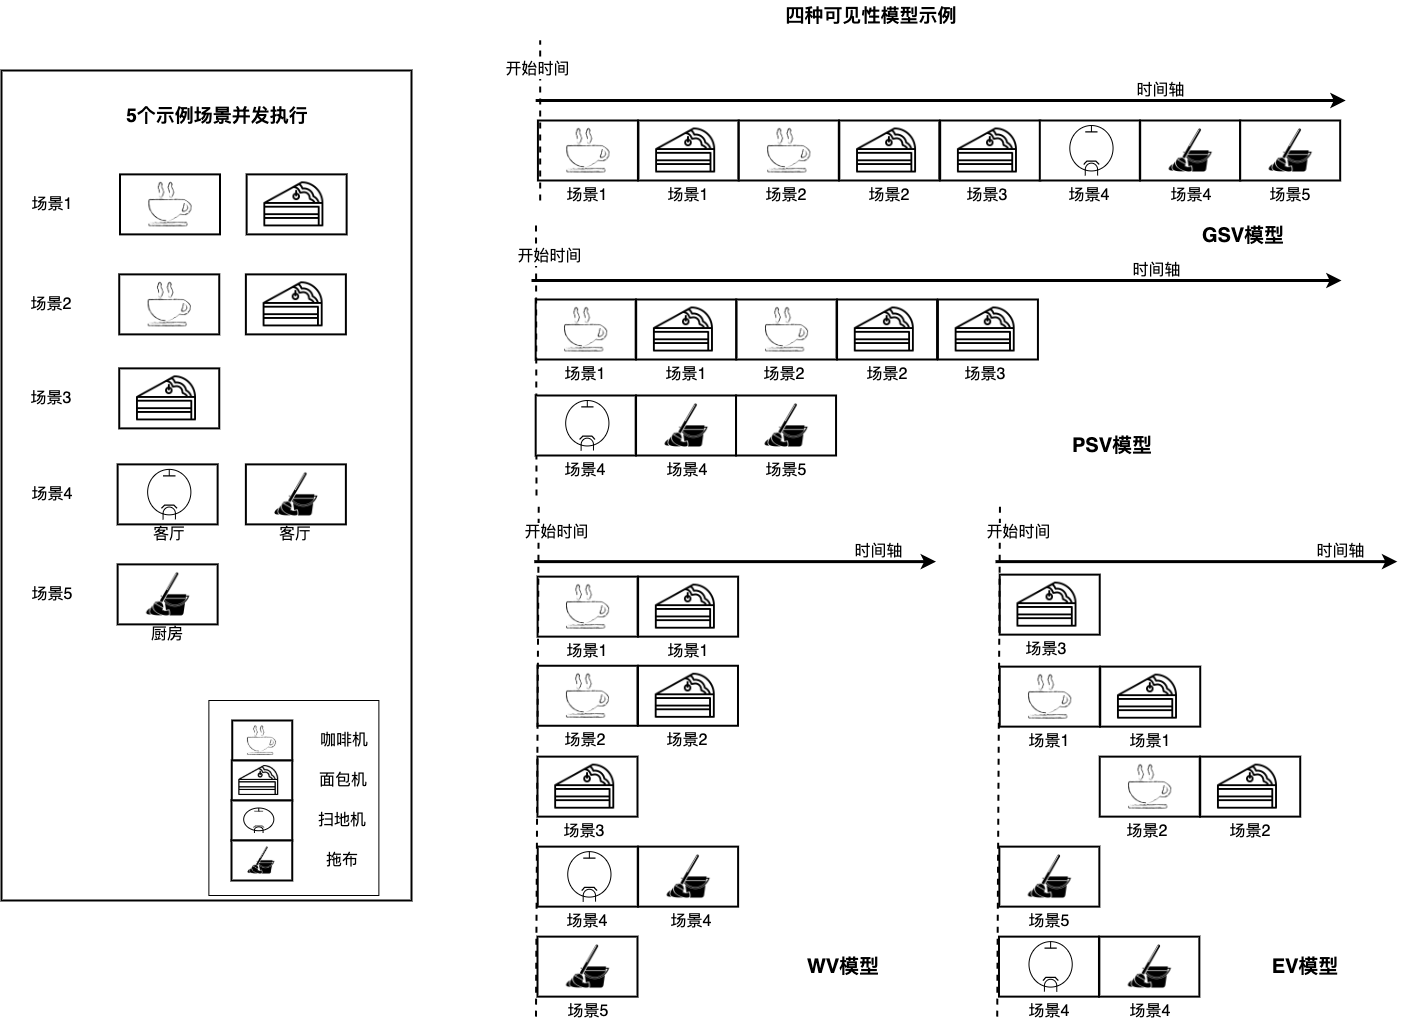
\includegraphics[width=1.0\textwidth]{figure/2-relatework/safehome.png}
	\caption{Safehome中的四种可见性模型示例}
	\label{ontransact-impl}
\end{figure}
\begin{itemize}
    \item \textbf{Global Strict Visibility (GSV) 模型}:GSV模型具有最强的原子性,当并发场景运行时,某一时刻只会运行单个场景,场景之间顺序执行,如图2-3中,五个场景顺序运行。GSV模型能够保证场景完整性和有序性,但是并发场景运行时阻塞时延高,无法保证场景高效性。
   \item \textbf{Partitioned Strict Visibility(PSV) 模型}:PSV模型是基于GSV模型的优化版本,在并发场景运行时,将不会互相影响的场景分离,单独执行,如图2-3中,场景1、2、3顺序运行,而场景4和场景5顺序运行。PSV模型同样能够保证场景完整性和有序性,相较于GSV模型,具有较好的场景高效性。
    \item \textbf{Eventual Visibility (EV) 模型}:EV模型保证场景的弱原子性,其策略是场景可以在不违背串行顺序的情况下并发执行,给IoT服务加锁,并通过Post/Pre-Lease机制保证场景的安全性,如图2-3中,场景3先执行,与此同时,场景1中的咖啡机服务可以同时运行,依此编排,具有最好的场景高效性。EV模型理论上是锁实现的最优模型,能够在保证场景全局安全性下,提供最好的执行延时表现,SafeHome的实验部分也证明了这一点。
    \item \textbf{Weak Visibility(WV) 模型}:WV模型无法保证场景的原子性,当场景触发时,直接执行,如图2-3中,五个场景同时执行,无法保证场景执行安全。因此当出现并发场景执行时,可能会出现并发冲突等问题,无法保证场景完整性和有序性。
\end{itemize}

本文认为,SafeHome在原子性定义上值得商榷,routine的原子性定义在某些具体场景下过于严苛,例如在\textit{洗衣服场景}中,会影响场景阻塞时间。SafeHome认为洗衣机场景是一个原子routine,那么当并发出现时,这种原子定义显然会影响执行效率(假设存在routineA和routineB并发执行,routineB可以在routineA中洗衣机运行结束后获取洗衣机服务,而无需等待整个routineA结束)。并且SafeHome中实验证明的最优的可见性模型在某种程度上挑战了SafeHome中的原子性定义,除此之外,SafeHome只提供了冲突处理框架的实现,没有实现一个完整的IoT服务组合框架。



\section{IoT服务组合冲突检测}

在IoT服务组合的冲突检测方面,主要思路是通过预先的冲突检测或预测来避免并发冲突的出现。Dipankar Chaki等人\cite{chaki2020conflict}\cite{chaki2020fine}\cite{huang2018convenience}考虑在智能家居的多用户(并发)场景中,基于用户们的历史行为数据,用深度学习的方式预测出用户们在某一时刻可能出现的对同一设备的并发访问情况,从而实现冲突避免。从理论层面,这样的冲突检测方式对冲突处理有很大的帮助,但是本文认为,首先基于深度学习的方式存在偶然性,其预测正确性在复杂场景中很难得到保证,此外智能家居的场景在冲突处理时考虑的因素比较清晰直观,理论上可以通过合理的系统实现和经典的冲突处理算法来解决,并不依赖于复杂的深度学习相关的预测模型。

\chapter{模型驱动的IoT服务组合建模方法}

模型驱动开发被认为是实现IoT管理系统高效构建和稳定运行的关键\cite{DBLP:journals/cse/FortinoGRS17},为了降低开发人员的开发负担,本文设计了一种模型驱动的IoT服务组合建模方法,并设计实现了相应的领域特定语言(DSL)—coraML。考虑到场景的执行过程本质上是一系列IoT服务内部运行状态的变更过程,所以本文基于IoT服务模型构建IoT服务组合模型,并将IoT服务的设备属性和状态转移逻辑分开考虑,分为IoT服务设备属性建模和IoT服务状态转移建模。

\section{模型驱动开发}
本文采用模型驱动开发来进行IoT服务组合框架的实现。模型驱动开发 (Model Driven Development,简称MDD)\cite{kent2002model} 是一种使用模型作为软件规范并转换这些模型以获得可运行文件或源代码的方法,MDD以构建软件系统模型为中心,其背后的核心是,通过创建系统模型,然后框架以动态解析或者代码生成等方式生成可运行的实际系统\cite{volter2009best},图3-1展示了MDD的基本开发流程,首先平台为用户提供一种模型语言,让用户对期望的最终实现进行模型定义;然后平台用代码生成,模型解析等方式对用户定义的模型进行模型转换;最后将模型转换后的系统输出,包括系统UI,API文档等。MDD为IoT服务管理系统开发带来了很多优势\cite{ModelDrivenSoftwareDevelopment}\cite{domingo2020evaluating}:
\begin{itemize}
    \item \textbf{提高代码质量}:MDD可以通过模型定义消解业务系统中原本复杂的业务逻辑,并且通过动态解析或者代码生成的方式进行系统实现,相较于开发人员编码实现的方式,会降低代码复杂度,减少系统中可能产生的错误,提升代码质量。
    \item \textbf{减少设计负担}:在MDD开发中,项目生成框架可以包含该领域中最佳的项目实践经验和最优的项目设计方案,所以项目开发可以带来业界相对优良的体系架构和实践经验,提升系统运行效率。
    \item \textbf{提升开发效率}:对开发人员来说,MDD中应用的模型是在比传统编程语言更高的抽象级别上指定的,这种语言更简单,易于理解。并且模型可以消解很多开发人员需要重复实现的固定逻辑,减少开发人员的工作量。
\end{itemize}
研究表明,MDD 将创建应用程序的工作量减少了 40-70\%,并且可以用更少的资源实现更多的功能\cite{parviainen2009model}。因此我们采用MDD来进行IoT服务组合框架的实现。

% 值得注意的是,MDD遵循领域驱动设计(DDD)的设计思想。DDD是由Eric Evans\cite{evans2004domain}最先提出,目的是对软件所涉及到的领域进行建模,以应对系统规模过大时引起的软件复杂性的问题\cite{ddd}。整个过程是这样的,开发团队和领域专家一起通过通用语言(Ubiquitous Language)去理解和消化领域知识,从领域知识中提取和划分为一个一个的子领域(核心子域,通用子域,支撑子域),并在子领域上建立模型,再重复以上步骤,这样周而复始,构建出一套符合当前领域的模型。模型设计聚焦于特定领域,不同领域的业务需求进行分析、抽象建模和技术框架分层所常用的分析方法就是DDD。

在MDD的开发流程中,模型定义(Model Definition)和模型转换(Model Transformation)是MDD中的核心流程,领域特定语言(Domain Specific Language,简称DSL)\cite{van2000domain}被用来进行模型定义,而模型转换往往通过代码生成平台或者模型翻译平台实现。对应于本文中的具体领域——IoT服务组合,本文提出的IoT服务组合建模方法就是针对IoT服务组合领域的模型定义方法,Cora框架可以被认为是MDD中的模型转换平台,本章则关注于IoT服务组合建模方法的阐述。

\begin{figure}
	\centering
	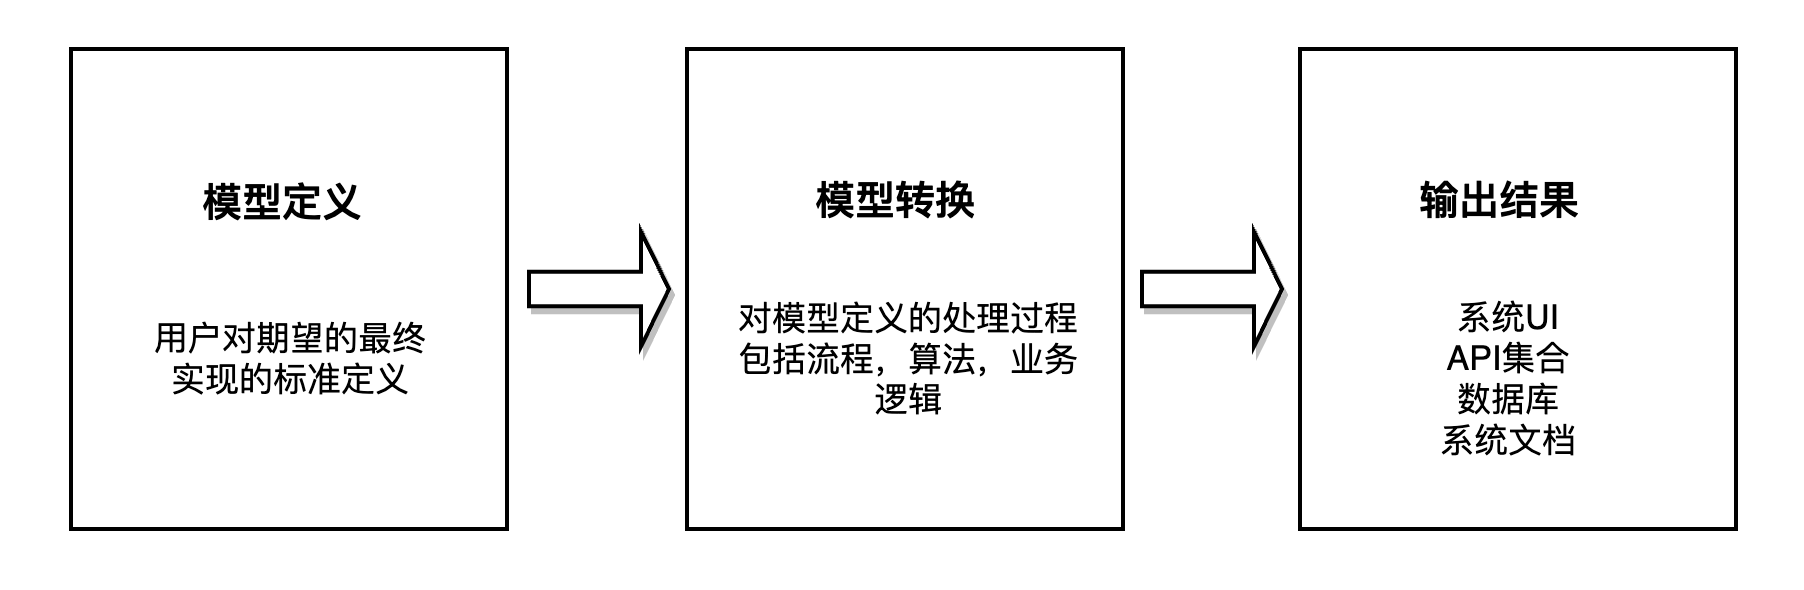
\includegraphics[width=1.0\textwidth]{figure/3-model-driven/MDD.png}
	\caption{模型驱动开发(MDD)流程}
	\label{ontransact-impl}
\end{figure}

\subsection{模型定义}
IoT服务组合建模方法聚焦于MDD中的模型定义,即开发人员通过模型定义来描述IoT服务组合场景。模型定义是MDD的基础和核心,模型包含对要构建的应用程序的领域知识和概念\cite{dsl}。对开发人员来说,可以将模型视为需求规范:你可以说明你的应用程序处理什么样的数据,应用程序实现的过程以及塑造最终应用程序的其他一些细节。

\subsection{领域特定语言—coraML}
DSL是模型定义的工具和信息载体。DSL是针对某一领域,具有受限表达性的一种计算机程序设计语言,DSL是在模型之上建议的一种更加灵活的对模型化的理解和使用方式,核心是语义模型。可以将DSL理解为针对某一特定领域一种声明式编程语言,针对网页显示的HTML语言,针对配置声明的YAML等都是DSL。
% DSL分为外部DSL和内部DSL:

% \textbf{外部DSL}是一种从应用程序主语言中分离出来的语言。通常来说,外部DSL采用自定义的语法,不过也常使用其他语言(如XML,JSON)的语法。应用程序使用文本语法分析技术来对外部DSL中的脚本进行解析,当然xtext等编程语言开发框架也封装了外部DSL的构建和解析工作,降低了外部DSL实现的难度。正则表达式,SQL等都是外部DSL。

% \textbf{内部DSL}是通用性语言的一种特定用法。用内部DSL编写的脚本在通用型语言(C,Java,JSON)中是合法代码,但是它仅以特定的风格使用通用型语言特性的一个子集,来处理整个系统中某个方面的问题。与外部DSL不同,内部DSL不需要学习文法和语言语法分析,但是会受到宿主语言的多方面限制。但是对于宿主语言能够支持的需求,借助内部DSL可以简单高效的实现。

图3-2展示了DSL的开发流程,设计DSL的核心是设计人与程序的交互逻辑,用户书写DSL,DSLParser进行解析,然后将解析结果以数据实例的形式存储在数据库或运行系统中,Interpreter 再去解析数据实例 执行相应的业务逻辑。DSL设计需要考虑很多方面,例如用户的书写体验,DSL的学习成本,程序的解析效率,DSL的扩展性等等\cite{dsldesign}。

\begin{figure}
	\centering
	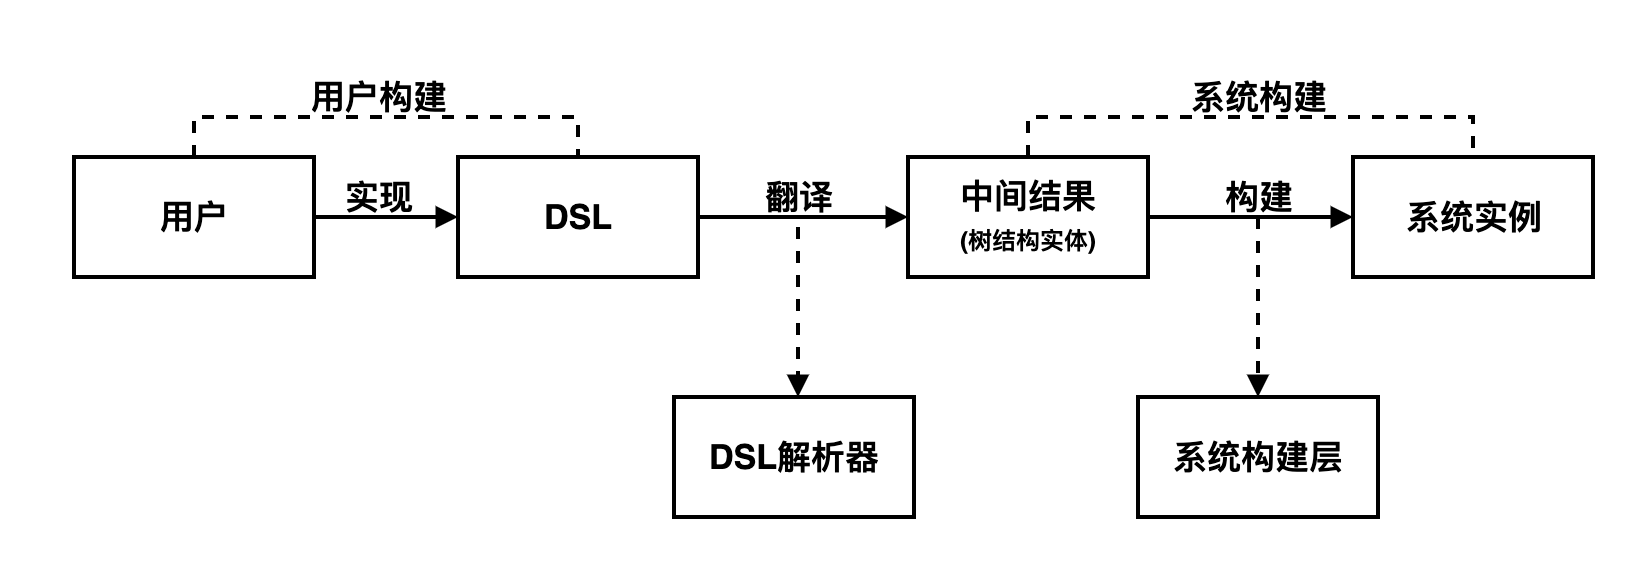
\includegraphics[width=1.0\textwidth]{figure/3-model-driven/dsl_lifecycle.png}
	\caption{DSL的开发流程}
	\label{ontransact-impl}
\end{figure}

Cora中基于JSON(JavaScript Object Notation)\cite{json}设计实现了一套DSL—coraML。JSON是一种轻量级的数据交换格式和声明语言,其表达能力很强,应用非常广泛。JSON对用户来说易于理解和表达,应用广泛;对项目开发来说易于解析和生成,语法解析器的实现相对简单。因此Cora中基于JSON设计实现了一套外部DSL—coraML。下文将结合模型构建过程,通过具体示例阐述coraML的具体设计和使用。
图3-3展示了\textit{洗衣服场景}的IoT服务组合模型图。
\begin{figure}
	\centering
	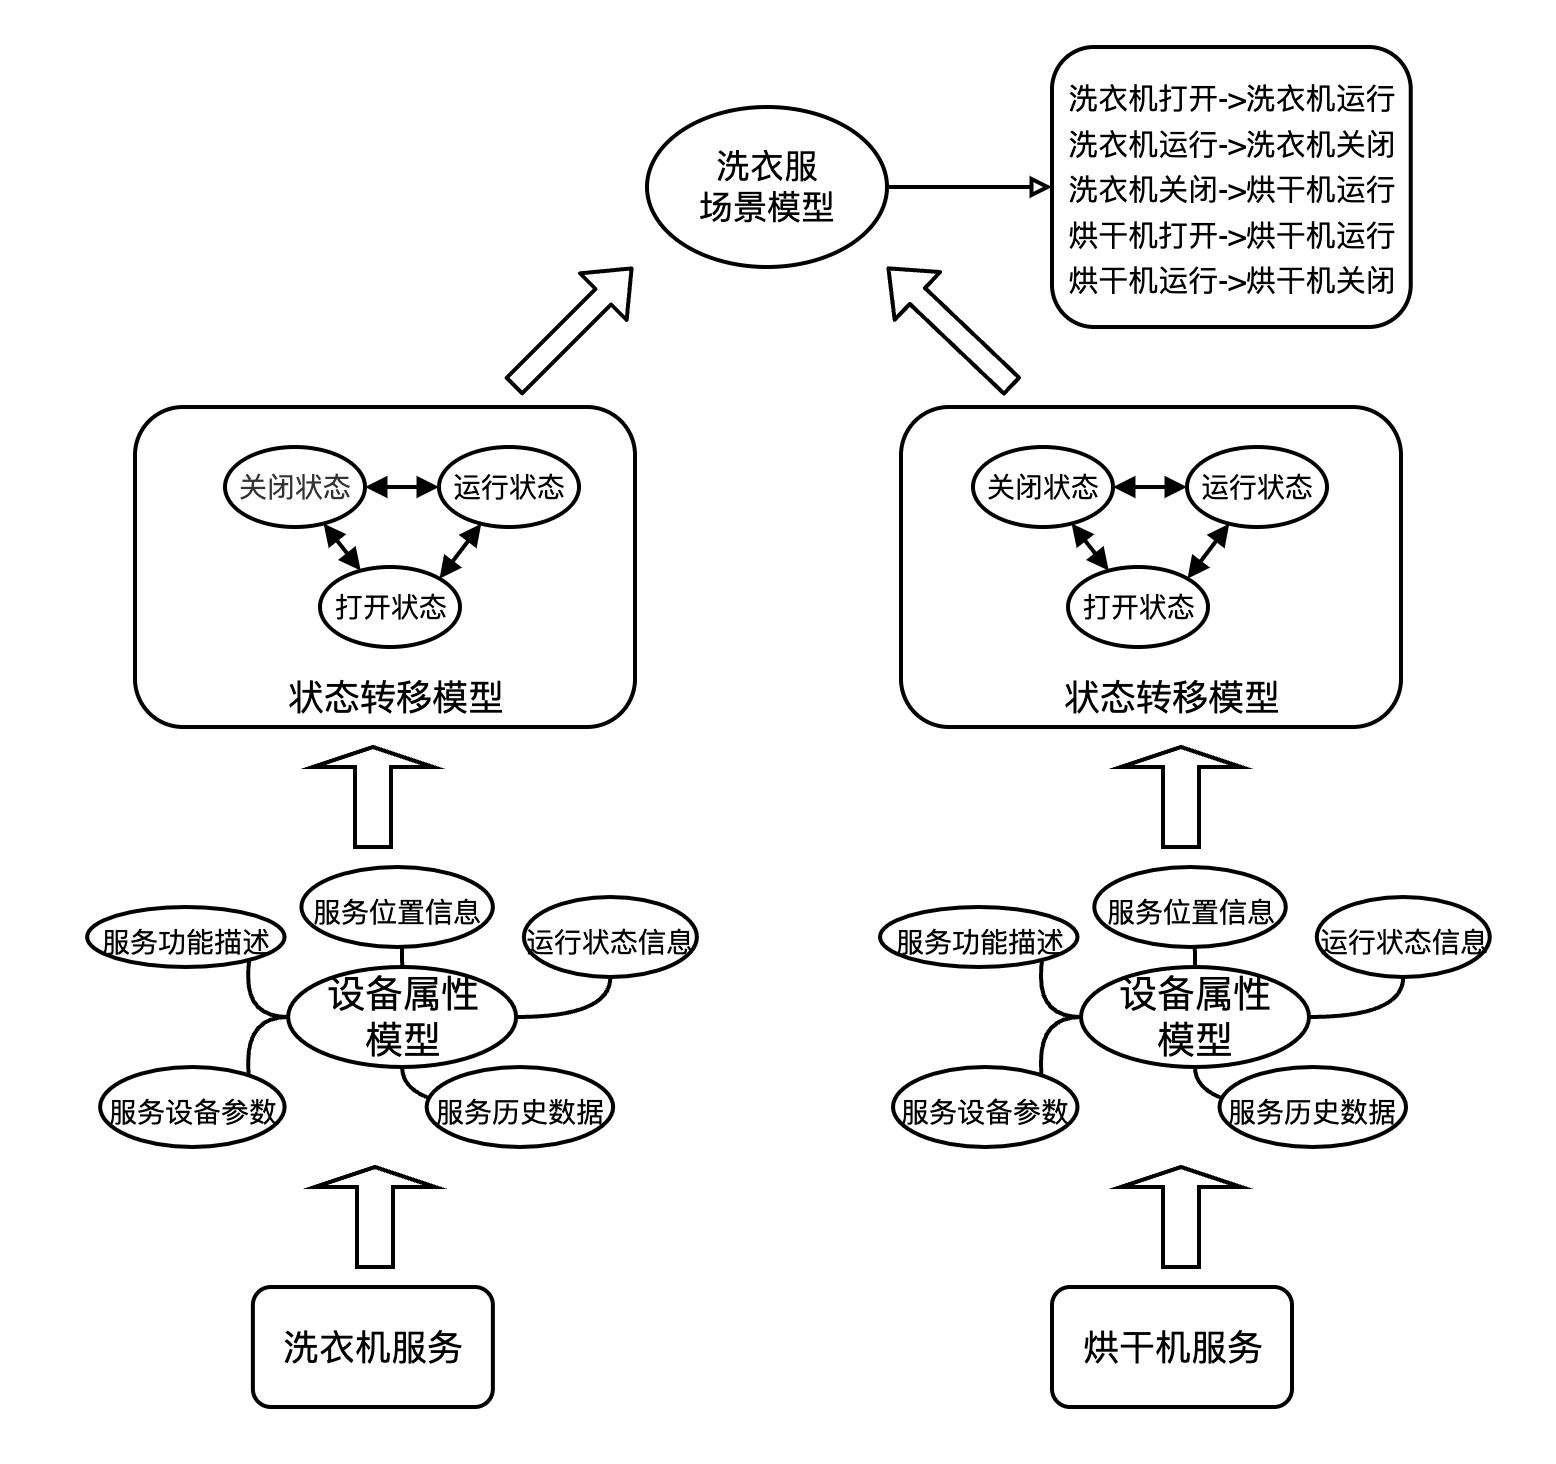
\includegraphics[width=1.0\textwidth]{figure/3-model-driven/example.png}
	\caption{\textit{洗衣服场景}的IoT服务组合模型图}
	\label{ontransact-impl}
\end{figure}

\section{IoT服务建模}
IoT服务建模是IoT服务组合建模的基础,开发人员可以通过定义IoT服务模型来完成IoT服务在服务组合场景中的注册。场景的执行过程本质上是一系列IoT服务内部运行状态的变更过程,而IoT服务自身的功能属性是构建场景组合逻辑的基础和前提。例如\textit{洗衣服场景}实际上是洗衣机服务和烘干机服务的运行过程,洗衣机服务和烘干机服务本身的功能属性是用户能够构建该场景的前提和基础,而场景模型则将这两个独立的IoT服务通过组合逻辑构建成一个整体。所以为了充分利用IoT服务的设备信息和运行逻辑来支撑场景的组合逻辑,IoT服务建模聚焦于IoT服务的设备属性和状态转移逻辑。

IoT服务的设备属性是构建场景组合逻辑的基础和前提。IoT服务具有很多内在信息,具体如图3-4展示,例如品牌,功能描述,位置信息,运行状态,历史记录,设备参数和控制逻辑等。本文将品牌,功能描述,位置信息,运行状态和设备参数等统一表示为IoT服务的设备属性,这些设备属性分为两种类型,一种是静态资源属性,以空气净化器服务为例,空气净化器服务的品牌,出厂参数,功能描述等不可变更的属性即为静态资源属性,开发人员可以基于静态资源属性来设计合理的场景组合逻辑;另一种是运行状态属性,空气净化器服务的运行状态,运行功率,转速等运行时属性即为运行状态属性,开发人员可以基于运行状态属性来监测场景的执行过程。两种类型的设备属性都可以通过静态字段定义,描述了IoT服务静止或运行时的状态信息,本文进行统一的定义和描述。

IoT服务的状态转移逻辑支撑场景运行。IoT服务的操控逻辑较为复杂,描述了IoT服务内部的状态转移过程,一般通过控制器来完成。本文将通过状态转移模型来进行描述。
\begin{figure}
	\centering
	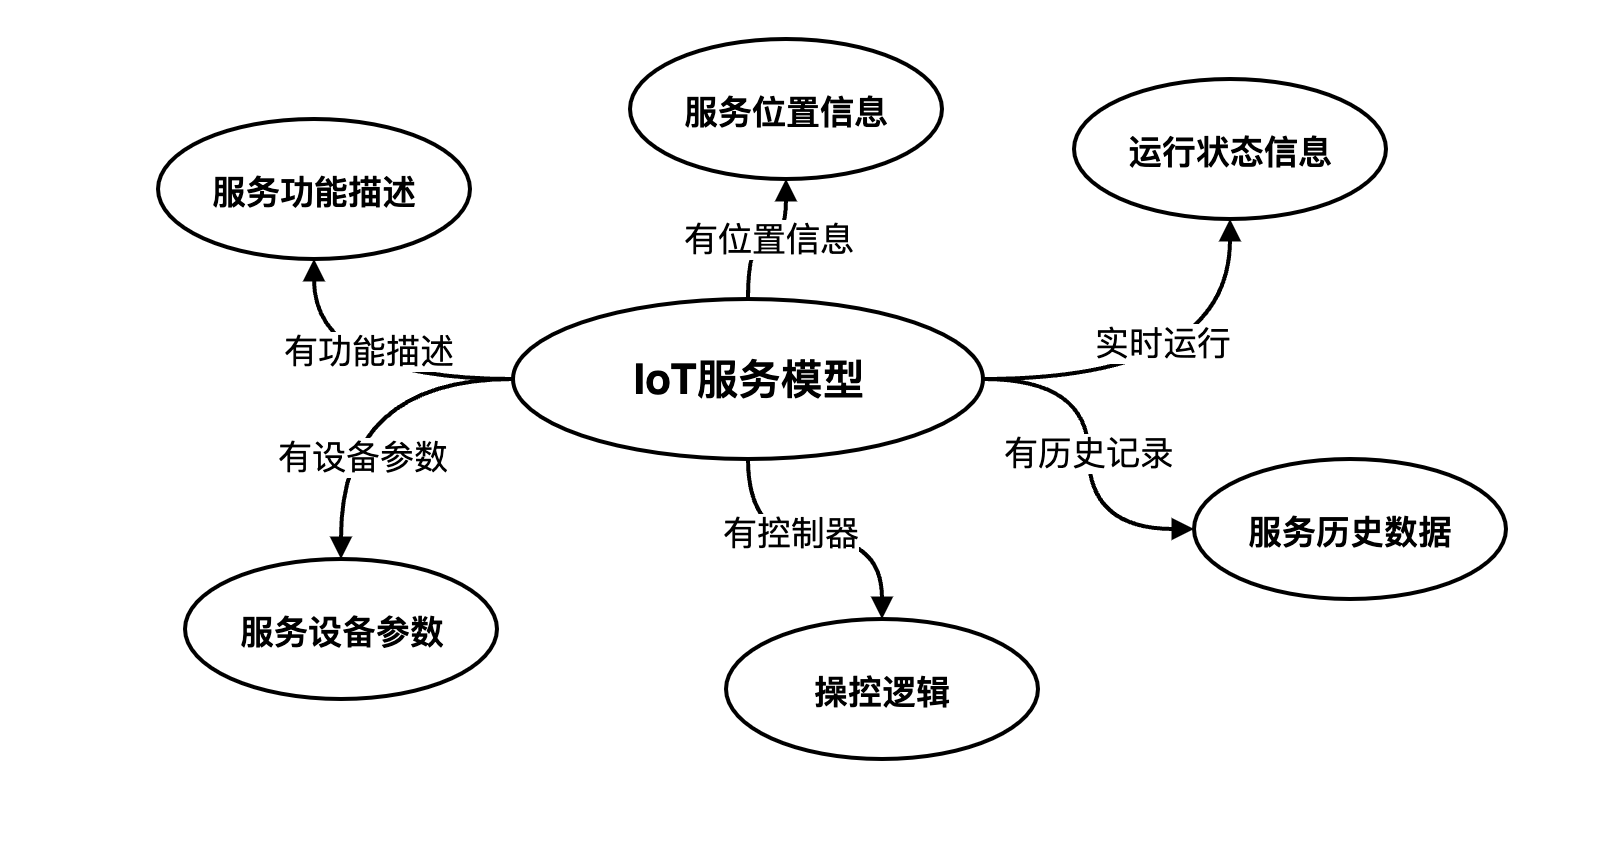
\includegraphics[width=1.0\textwidth]{figure/3-model-driven/device_description_model.png}
	\caption{IoT服务的描述模型}
	\label{ontransact-impl}
\end{figure}


\subsection{IoT服务设备属性建模}
IoT服务自身的静态资源属性是构建场景组合逻辑的基础和前提,运行状态属性则标识了场景中IoT服务的实时状态和运行数据,两者缺一不可。IoT服务的设备属性模型定义如下:

定义1: 定义$\sum attr$为IoT服务$K$的设备属性集合,$\sum attr\_static$为$K$的静态资源属性集合,$\sum attr\_dynmaic$为$K$的运行状态属性集合。

\begin{align}
\sum attr\_static \bigcap \sum attr\_dynmaic = \varnothing \label{1} \\
\sum attr = \sum attr\_static \bigcup \sum attr\_dynmaic   \label{2}
\end{align}

% $$ \sum attr\_static \bigcap \sum attr\_dynmaic = \varnothing ;  \label{1} $$
% $$ \sum attr = \sum attr\_static \bigcup \sum attr\_dynmaic   \label{2} $$

基于上述IoT服务设备属性模型,coraML中基本的设备属性类型有:string,integer,float,boolean,特殊类型有object和link。
\begin{itemize}
  \item [1)] 
  object:表示一个IoT服务类型,解析器解析object类型时会将其解析为一个新的IoT服务类型。 
  \item [2)]
  link:考虑到IoT服务之间存在组合情况,所以coraML提供了关联语义的定义,在定义object的某个属性时,可以通过link关联到某个具体IoT服务实例。
\end{itemize}
以\textit{洗衣服场景}中的净化器服务为例,代码3.1展示了coraML定义的IoT服务设备属性模型。
% \definecolor{delim}{RGB}{20,105,176}
% \definecolor{numb}{RGB}{106, 109, 32}
% \definecolor{string}{rgb}{0.64,0.08,0.08}

% \lstdefinelanguage{json}{
%     numbers=left,
%     numberstyle=\small,
%     frame=single,
%     rulecolor=\color{black},
%     showspaces=false,
%     showtabs=false,
%     breaklines=true,
%     postbreak=\raisebox{0ex}[0ex][0ex]{\ensuremath{\color{gray}\hookrightarrow\space}},
%     breakatwhitespace=true,
%     basicstyle=\ttfamily\small,
%     upquote=true,
%     morestring=[b]",
%     stringstyle=\color{string},
%     literate=
%      *{0}{{{\color{numb}0}}}{1}
%       {1}{{{\color{numb}1}}}{1}
%       {2}{{{\color{numb}2}}}{1}
%       {3}{{{\color{numb}3}}}{1}
%       {4}{{{\color{numb}4}}}{1}
%       {5}{{{\color{numb}5}}}{1}
%       {6}{{{\color{numb}6}}}{1}
%       {7}{{{\color{numb}7}}}{1}
%       {8}{{{\color{numb}8}}}{1}
%       {9}{{{\color{numb}9}}}{1}
%       {\{}{{{\color{delim}{\{}}}}{1}
%       {\}}{{{\color{delim}{\}}}}}{1}
%       {[}{{{\color{delim}{[}}}}{1}
%       {]}{{{\color{delim}{]}}}}{1},
% }
\colorlet{punct}{red!60!black}
\definecolor{background}{HTML}{EEEEEE}
\definecolor{delim}{RGB}{20,105,176}
\colorlet{numb}{magenta!60!black}

\lstdefinelanguage{json}{
    basicstyle=\normalfont\ttfamily,
    numbers=left,
    numberstyle=\scriptsize,
    stepnumber=1,
    numbersep=8pt,
    showstringspaces=false,
    breaklines=true,
    frame=lines,
    backgroundcolor=\color{background},
    literate=
     *{0}{{{\color{numb}0}}}{1}
      {1}{{{\color{numb}1}}}{1}
      {2}{{{\color{numb}2}}}{1}
      {3}{{{\color{numb}3}}}{1}
      {4}{{{\color{numb}4}}}{1}
      {5}{{{\color{numb}5}}}{1}
      {6}{{{\color{numb}6}}}{1}
      {7}{{{\color{numb}7}}}{1}
      {8}{{{\color{numb}8}}}{1}
      {9}{{{\color{numb}9}}}{1}
      {:}{{{\color{punct}{:}}}}{1}
      {,}{{{\color{punct}{,}}}}{1}
      {\{}{{{\color{delim}{\{}}}}{1}
      {\}}{{{\color{delim}{\}}}}}{1}
      {[}{{{\color{delim}{[}}}}{1}
      {]}{{{\color{delim}{]}}}}{1},
}


\begin{lstlisting}[caption={coraML定义的净化器服务的设备属性模型},label={lst:airpurifier_device_model},language=json,basicstyle=\footnotesize] 
{
    fieldschema: {
      type: object,
      nodeType: AirPurifier, //IoT服务模型名称
      properties: {
        purifierId: {
          type: string ,
          title: 编号
        },
        speed: {
          type: integer,
          title: 速度
        },
        isRunning: {
          type: boolean,
          title: 是否工作
        },
        sensor: {   //关联传感器服务实例
          type: link,
          title: 传感器实例
        }}}
 }
\end{lstlisting}



\subsection{IoT服务状态转移建模}
IoT服务的状态转移是场景运行的基础。因为场景的执行过程本质上是一系列IoT服务内部运行状态的变更过程,而场景的组合逻辑促成了独立的IoT服务的状态转移逻辑之间的连接,因此IoT服务的状态转移是场景运行的基础。但是通过编码的方式实现IoT服务的状态转移逻辑不符合MDD的理念,也会增加开发人员的开发负担,因此本文为IoT服务的状态转移逻辑建模。

本文采用有限状态机模型来为IoT服务的内部状态转移逻辑建模,IoT服务的特性和框架的实现需求决定了其合理性和可行性。一方面来说,IoT设备往往被设计来完成某项单独具体的功能,例如洗衣机用来洗衣服,热水器用来烧水,因此其可能的运行状态是有限的,在开发制造时生产商通过简单的电子控件便可实现IoT设备的状态转移管理,换言之,可以认为IoT设备本身就是一种物理的有限状态机\cite{drumea2004finite},因此与之对应的大部分IoT服务的内在运行逻辑也是相对简单直观的。另一方面对于模型构建来说,基于“the rule of least power”原则\cite{theruleofleastpower},Cora需要一种尽可能没有冗余,简单直观的建模方式来对IoT服务的状态转移建模。相关研究表明,由web服务组成的web系统可以基于有限状态机建模实现\cite{zuzak2011finite}\cite{zuzak2011formal},基于这个思路,本文认为相较于大部分web服务,IoT服务的状态数量要更少,并且状态转移逻辑相较于大部分web系统来说也要简单很多,因此本文决定
基于有限状态机模型来为IoT服务的状态转移逻辑建模。

\paragraph{有限状态机模型}
有限状态机(Finite State Machine,简称FSM )\cite{fsmwiki}是一种计算的数学模型,由状态列表、初始状态和触发每个transition的输入定义。它是一个抽象的机器,在任何给定的时间都可以处于有限个状态(state)中的一个。FSM可以根据某些输入从一种状态切换到另一种状态;从一种状态到另一种状态的变化称为transition。有限状态机有两种类型:确定性有限状态机和非确定性有限状态机。确定性有限状态机可以被构造成等价于任何非确定性有限状态机。
有限状态机建模可以被认为是一种状态驱动的建模方式。在软件工程中,状态由一组变量和特定值定义。通过这种方式,IoT设备频繁从一种物理状态跳到另一种物理状态的固有行为模式,可以一致地映射到虚拟网络中能够不断发生规律性状态转移的状态模型驱动的虚拟服务。在有限状态机模型构建流程中,首先声明服务的所有状态(state)和初始状态(initState),并用一组变更(transition)描述这种规律性的状态转移,最后模型实例通过event来驱动状态机运转。

有限状态机建模(Finite State Machine Modeling)\cite{fsm}是一种通过显示系统的每个可能状态以及状态之间的转换关系来进行系统建模的方式。基于有限状态机的模型在电子工程和控制系统中用于设计和仿真目的已有很长的历史。然而,在IoT服务建模领域,这样的工作才刚刚开始。理论上,基于FSM的模型描述简单,语义能够支持IoT服务的需求,同时也可以使用语义描述来提高互操作性。

\paragraph{IoT服务状态转移模型}

本文基于NFA模型对IoT服务状态转移模型的定义如下:

定义2:定义$S_k$为IoT服务$K$的所有状态的集合,$s_i$\in $S_k$,0<$i$<$n$,$n \in Z $,$s_0$为$K$的初始状态。

定义3:定义$\sum k$是$K$接收事件的集合,$e_i$ \in $\sum k$,0<$i$<$n$,$n \in Z $。

定义4:定义$T$为$K$的一次状态转移,假设$s_1$和$s_2$是$S_k$的两个内部状态,$$T: s_1\in S_k \rightarrow s_2\in S_k $$。

定义5:定义$\delta$是$K$的状态转移函数,$$\delta: S_k  \times  \sum k \rightarrow S_k $$

% $$ S_{airpurifier}:[s_{off},s_{on},s_{low\_speed},s_{high\_speed}], s_0 : s_{off} $$
% $$ s_0 : s_{off} $$
% $$ \sum_{airpurifier}: [e_{turn\_on},e_{turn\_off},e_{speed\_up},e_{low\_speed} $$
% $$ \delta:[{s_{off} \stackrel{e_{turn\_on}}{\longrightarrow}  s_{on}}, 
% s_{on}|s_{low\_speed} \stackrel{e_{speed\_up}}{\longrightarrow}  s_{high\_speed},
% s_{on}|s_{high\_speed} \stackrel{e_{low\_speed}}{\longrightarrow}  s_{low\_speed},
% s_{on}|s_{low\_speed}|s_{high\_speed} \stackrel{e_{turn\_off}}{\longrightarrow}  s_{off},
% ] 
% $$

下面本文以空气净化器服务为例,解释Cora中用有限状态机为IoT服务状态转移建模的过程,图3-5展示空气净化器服务的FSM模型,图3-6展示了净化器服务的状态转移模型。有限状态机的核心包括state,initState,event和transition,并通过event和transition列表来描述各种状态之间的转换过程\cite{scxml}。例如图3-5中的空气净化器服务,在现实中,空气净化器有四种物理状态,分别是关闭状态,运行状态,低速运行状态和高速运行状态,按照实际运转逻辑,用户可以通过遥控器或物理按钮发送打开信号,将空气净化器从关闭状态转换成运行状态,用同样的方式操控净化器在运行状态,低速状态和高速状态之间相互切换,注意关闭状态只能和运行状态互相转换,这种约束也是Cora中对IoT服务状态转移建模的意义所在。相应地,在IoT服务场景中,本文用off,on,low\_speed和high\_speed四种state来描述空气净化器服务的四种状态,并在每种状态中,用turn\_on,turn\_off,speed\_up,speed\_low四种event来描述IoT服务可能接收的信号,同时用event和一组transition列表来描述空气净化器服务在该状态下可能的转换操作。
\begin{figure}
	\centering
	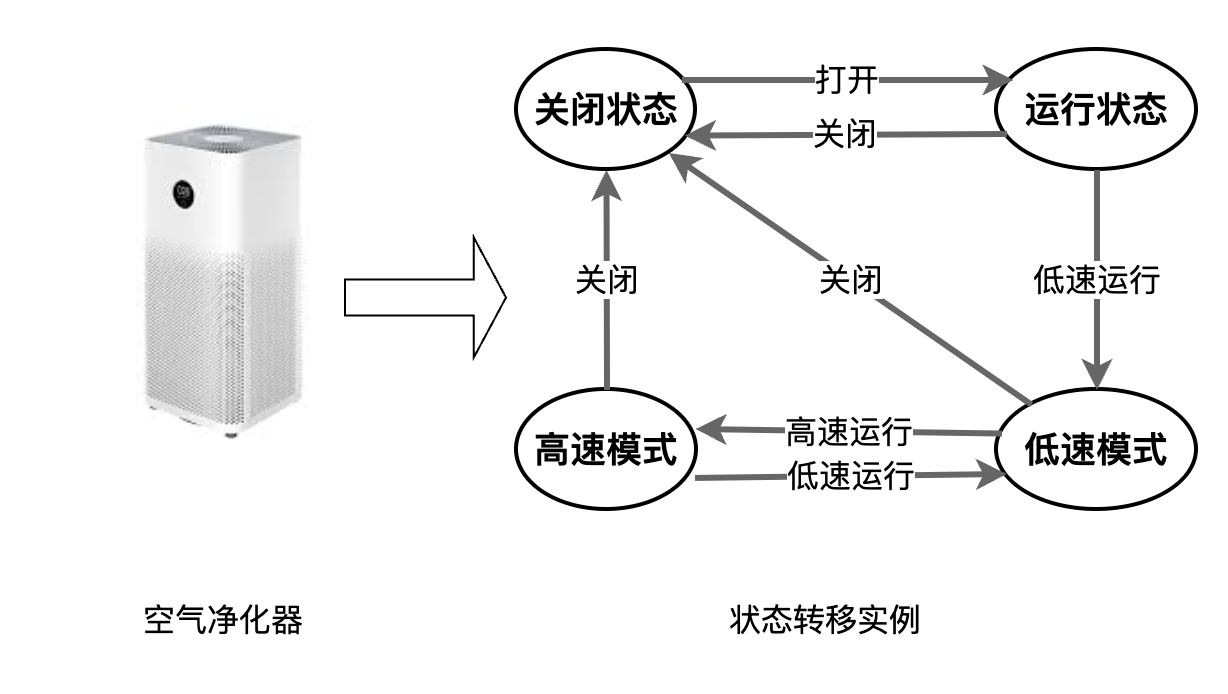
\includegraphics[width=0.8\textwidth]{figure/3-model-driven/fsm_for_airpurifier_1.png}
	\caption{净化器服务的FSM模型}
	\label{ontransact-impl}
\end{figure}
\begin{figure}
	\centering
	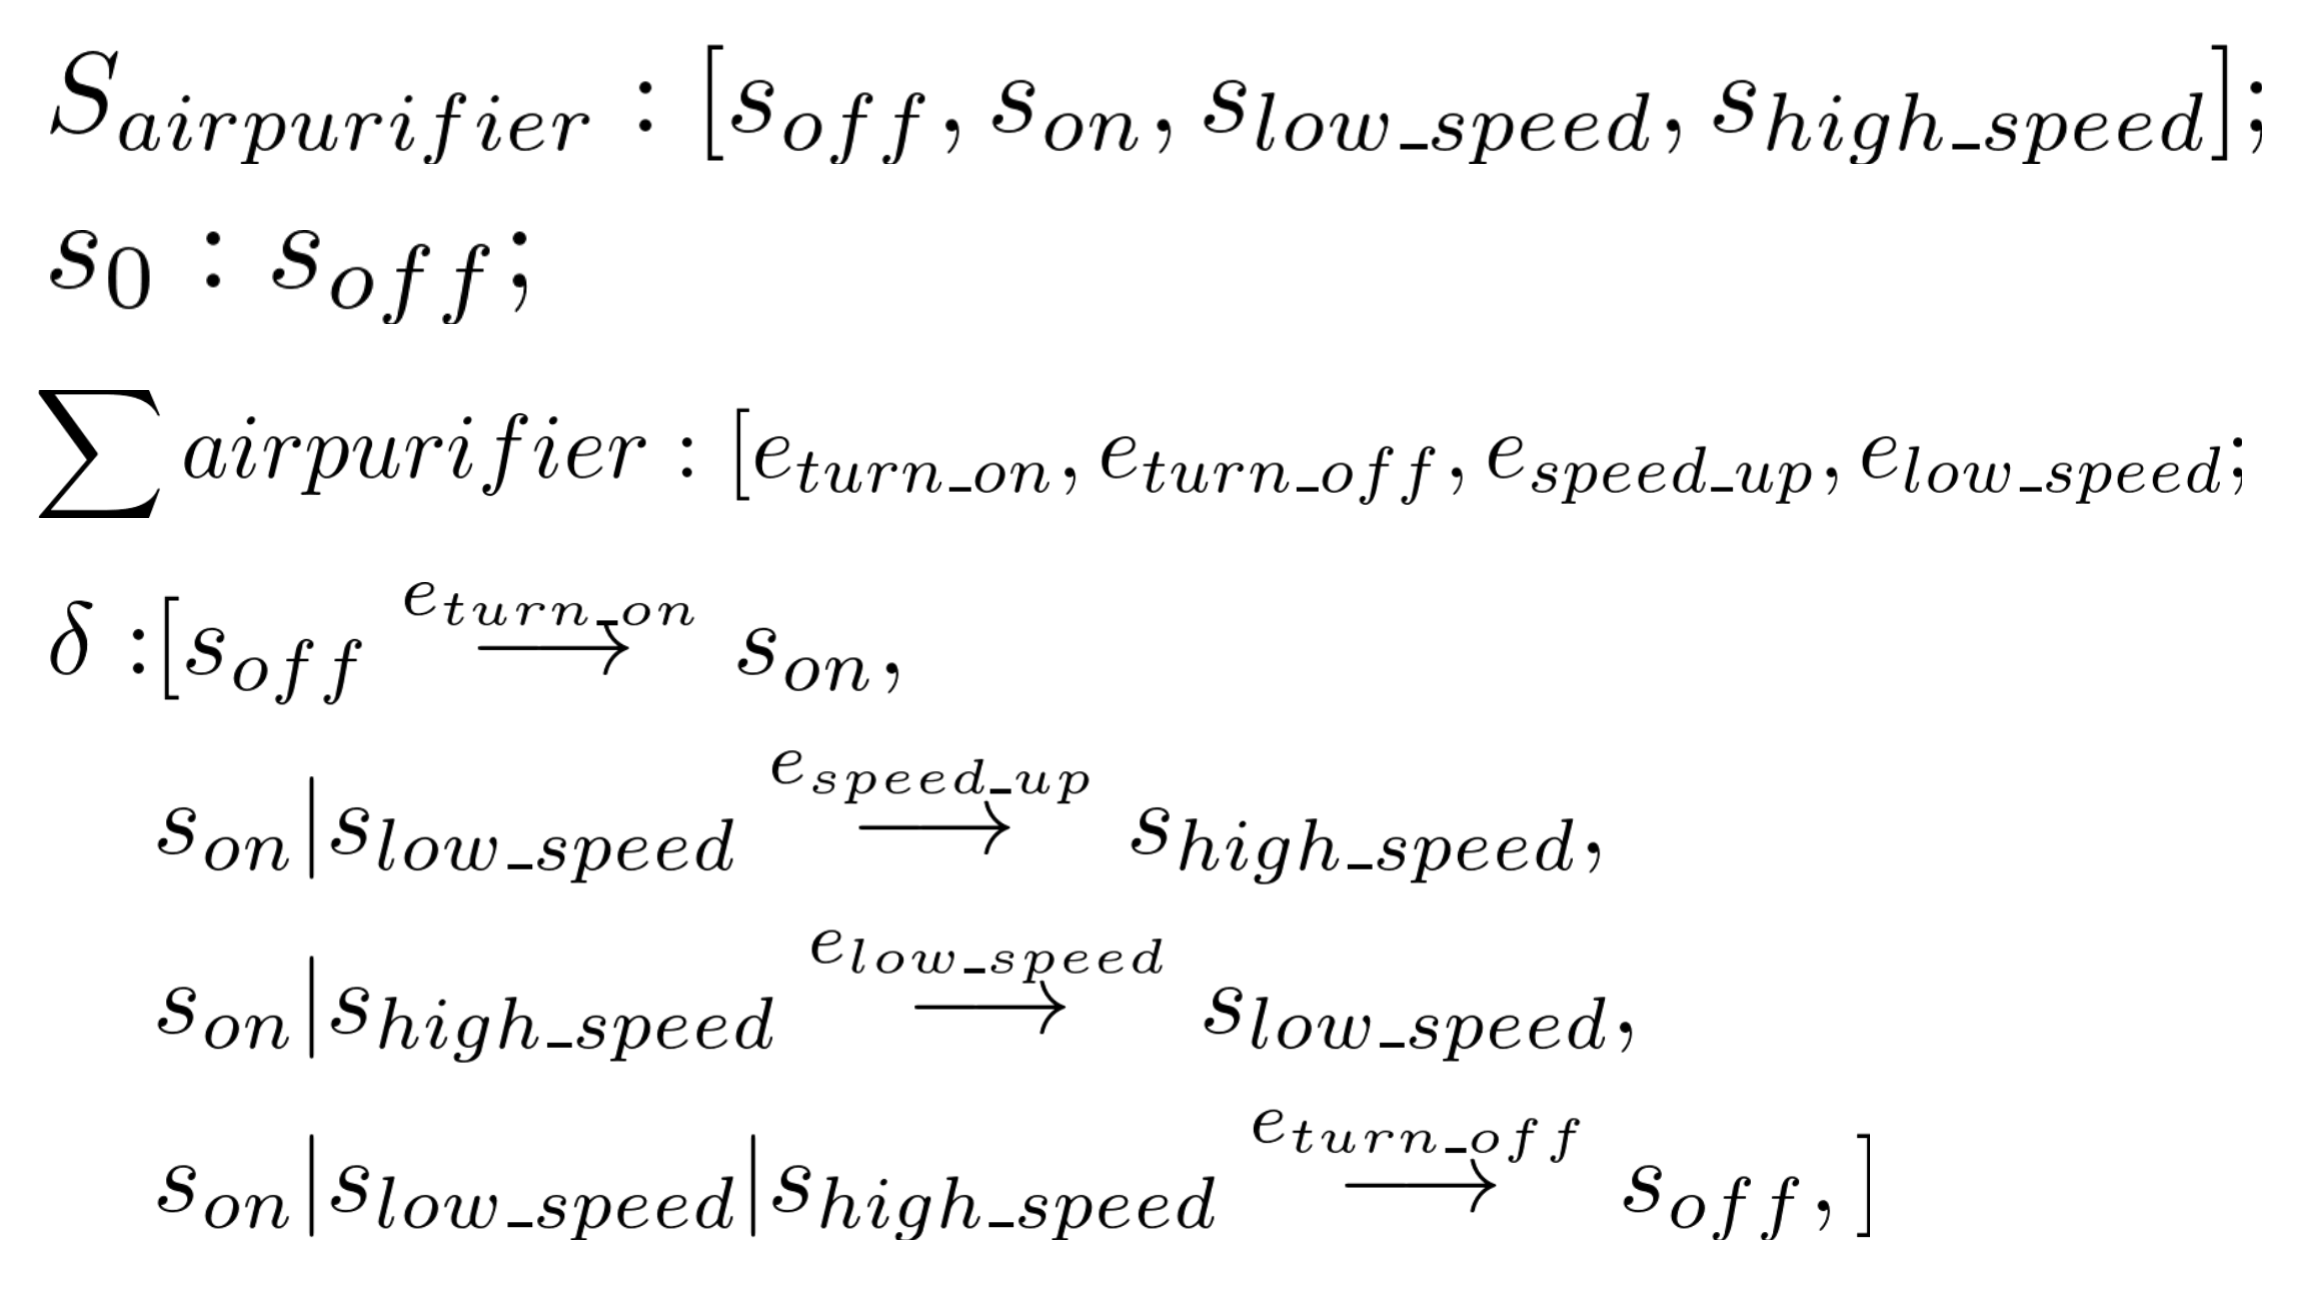
\includegraphics[width=0.7\textwidth]{figure/3-model-driven/fsm_for_airpurifier_2.png}
	\caption{净化器服务的状态转移模型}
	\label{ontransact-impl}
\end{figure}

coraML中遵循上述定义进行设计实现,代码3.2展示了coraML定义的IoT服务状态转移模型。coraML通过fsm字段声明有限状态机模型,states字段表示了有限状态机的所有state集合,startWith标识了有限状态机的初始状态,transitions字段标识了状态转移列表,每个实例中包含event,from,to三个字段:event标识了事件名称,from和to字段共同构建了在有限状态机接收到具体event时的一组多对一的状态转移标识。

\begin{lstlisting}[caption={coraML定义的净化器服务的状态转移模型},label={lst:airpurifier_transition_model},language=json,basicstyle=\footnotesize] 
{
    fieldschema: {...}
    fsm: {
        states: [off,on,low_speed,high_speed],
        startWith: off,
        transitions: [
            {
                event: turn_on,
                from: [off],
                to: on
            },{
                event: speed_up,
                from: [on,low_speed,high_speed],
                to: high_speed
            },{
                event: low_speed,
                from: [on,low_speed,high_speed],
                to: low_speed
            },{
                event: turn_off,
                from: [on,low_speed,high_speed],
                to: off
            }
        ]
    }
}
\end{lstlisting}

\section{IoT服务组合建模}
IoT服务组合模型基于IoT服务设备属性模型和IoT服务状态转移模型实现,开发人员可以通过定义IoT服务组合模型完成具体的场景的构建。
用模型驱动的方式来定义IoT服务组合是IoT服务组合建模领域的热门话题,总结来看,主要有如下几种方式:
\begin{itemize}
    \item  \textbf{基于编码的服务组合模型}:
    基于编码的服务组合是IoT服务组合中使用最直接最广泛的服务组合方式,一方面是因为目前大部分的IoT服务管理平台主要关注的是单个设备的连接管理,另一方面基于编码的服务组合方式也是最直接的开发方式。这种开发方式本质上是一种过程式开发,基于原始业务模型实现。并且这种方式在技术上要求很高,开发人员除了服务组合逻辑的实现,还需要考虑并发处理,错误处理等很多问题。
    \item  \textbf{基于规则/流程的服务组合模型}:
    基于规则/流程的服务组合模型在基于编码的服务组合模型之上做了一定的封装,本质上是一种业务流程驱动的组合模型。这种模型主要参考web服务组合中已经成熟的一些流程框架,如bpmn模型\cite{bpmn},可以将IoT服务组合逻辑用任务,活动等概念进行封装,降低了建模的复杂性。但是具体实现时,开发人员会通过任务来封装服务指令,从而构建出一系列服务指令的执行流程,在这种方式下,服务组合逻辑会变得弱化,退化为一系列被动执行的指令列表,在流程执行时,流程模型也无法将IoT服务特性与服务组合逻辑解耦开,换言之开发人员仍然需要考虑服务组合场景带来的场景完整性和场景阻塞时间等因素。
    \item  \textbf{数据驱动的服务组合模型}:
    数据驱动的服务组合模型主要应用于有流式数据处理的大数据IoT场景,例如智慧城市,智慧物流中的数据统计等,ThingsBoard中的服务组合采用这种建模方式。这种场景下的服务组合模型关注于数据的收集和展示,IoT服务之间的交互逻辑相对简单直白,在智能家居场景下并不适用。
    \item  \textbf{事件/消息驱动的服务组合模型}:
    事件驱动模型\cite{levina2009realizing}适用于分布式系统,通过在分布式系统内部传递消息的方式实现业务逻辑。这种模型可以将复杂系统充分解耦,并且很好地消解了分布式系统中可能出现的冲突问题\cite{scheer2005process}。
\end{itemize}

Cora中采用事件驱动的服务组合模型。本文认为IoT服务之间需要通过一种主动交互的方式驱动场景执行,因为IoT服务组合实质上是一种服务协同过程,而考虑到IoT设备的运行逻辑,IoT服务应该处于一种\{接收信号$\Rightarrow$完成操作$\Rightarrow$反馈信号\}的循环过程中,那么在保证IoT服务循环运行逻辑的前提下,IoT服务之间的协同过程应该表现为:\{IoT服务A:接收信号$\Rightarrow$完成操作$\Rightarrow$反馈信号;协同逻辑定义IoT服务B对IoT服务A的反馈信号作出反应; IoT服务B:接收反馈信号$\Rightarrow$完成操作$\Rightarrow$反馈信号\},该过程与事件驱动模型是完全匹配的。例如对于\textit{洗衣服场景},当洗衣机服务反馈关闭洗衣机服务的信号时,场景接收到该反馈信号,应该将该信号发送给对应的烘干机服务,从而完成整个场景。因此在事件驱动模型下,IoT服务组合模型只需关注该协同逻辑,即“当场景接收到反馈信号后应该发送给哪个IoT服务什么样的操作信号”,该协同逻辑可以由开发人员预先定义。
事件驱动的服务组合模型可以保证场景中IoT服务之间的充分解耦,维护了IoT服务的内部运行逻辑,并将IoT服务之间的组合逻辑通过事件和场景模型描述,因此本文采用事件驱动的服务组合模型。

IoT服务组合建模主要包括事件建模和场景建模两部分,事件建模主要目的是构建一种标准的交互协议—事件,在IoT服务内部以及IoT服务之间传递,IoT服务能够解析事件,并根据事件语义推动IoT服务的有限状态机运转。场景建模的主要目的是提供给开发人员一种标准的场景模型规范,能够通过coraML描述场景中IoT服务之间的组合协同逻辑。事件和场景模型共同推动场景向前运转。

\subsection{事件模型}
Cora中基于事件模型构建IoT服务之间以及IoT服务内部的标准交互协议,IoT服务可以发送事件给其他IoT服务,也可以接收来自外部或者其他IoT服务发送的事件,从而推动IoT服务向前运转。基于IoT服务的特性,Cora中将事件分为两种类型:\textbf{命令型事件}和\textbf{过程型事件},两者的主要区别在于事件是否有持续执行时间。举例来说,打开灯或者打开门这样的事件是以命令型式存在的,其执行时间可以忽略不计,所以在Cora中将其定义为命令事件;而洗衣机工作30分钟,净化器低速运行1小时这样的事件带有一段不可忽略的持续执行时间,所以在Cora中将其定义为过程型事件,两种事件类型会影响IoT服务的实际运行。

本文事件模型的定义如下:

定义6:定义$e$是IoT服务K接收的命令型事件;$e_{d,t}$是IoT服务接收的持续型事件,$t$为事件的执行时间。

$$ e_{d,t}|e  \times S_k \rightarrow S_k$$

以空气净化器服务的打开事件和低速运行10分钟事件为例,代码3.3展示了coraML定义的命令型时间和持续型事件两种事件模型。coraML中eventName字段表示事件名称,nodeType和instanceId共同指定了具体的IoT服务实例,data属性表示了事件中对IoT服务实例状态属性的更新,为object类型,isDuration字段用来区分命令事件和持续型事件,若isDuration为true,则声明duration来标识执行时间。
\begin{lstlisting}[caption={coraML定义的净化器服务的事件模型},label={lst:airpurifier_event_model},language=json,basicstyle=\footnotesize] 
//净化器服务的打开事件定义
{
    eventName:turn_on,
    nodeType:AirPurifier,
    instanceId:619892261336552,
    isDuration:false,
    data:{
        isOn: true
    }
}
//净化器服务的低速运行10分钟事件定义
{
    eventName:speed_low,
    nodeType:AirPurifier,
    instanceId:619892261336552,
    isDuration:true,
    duration:10000,
    data:{
        speed: 50
    }
}
\end{lstlisting}


\subsection{场景模型}
场景模型描述了IoT服务之间的组合逻辑,在消息驱动模型中,IoT服务之间的组合逻辑通过接收消息和发送消息(pub/sub模式)来实现,首先场景实例由外部事件(即用户或定时任务)启动,场景中的IoT服务会持续监听消息,外部事件会经由场景发送给的具体IoT服务,IoT服务接收外部事件,完成业务逻辑后根据场景模型定义,会将相应事件发送给其他IoT服务或IoT服务列表,循环整个过程直至场景实例执行结束。

本文的场景模型定义如下:

定义7:定义$C_i$为场景$A$在某一时刻的全局状态,0<$i$<$n$,$n \in Z $,$C_f$为$A$的最终状态,$C_{exe\_end}$为$A$运行的终止状态。

定义8:定义$N$为IoT服务$K$内部的一次状态转移,$N$不会更改$A$的状态,假设$s_1$和$s_2$是$K$的两个内部状态,$$N: s_1\in C_i \rightarrow s_2\in C_i $$

定义9:定义$M$为$A$的一次状态变更,假设存在两个不同的变量$i$,$j$,
$$ s_1\in C_i and s_2 \in C_{j\neq i} : M_{i,j} : s1\in C_i \rightarrow s2\in C_{j \neq i}$$

定义10:$A$的执行过程可以定义为一系列的状态$s_0$,$s_1$,$s_2$,$s_3$的变更过程。例如\textit{洗衣服场景}即为:
$$s_0\in C_1 \stackrel{N}{\longrightarrow} s_1 \in C_1 \stackrel{N}{\longrightarrow} s_2 \in C_1 \stackrel{M_{1,2}}{\longrightarrow} s_3 \in C_2 \stackrel{N}{\longrightarrow} s_4 \in C_2 \stackrel{N}{\longrightarrow} s_5 \in C_f = C_{exe\_end}$$

定义11:场景完整性定义:
场景$A$具有完整性当且仅当$$
C_{exe\_end} = C_f $$

定义12:场景有序性定义:

假设场景$A$具有事件$s_{a1}$,$s_{a2}$,$\cdots$,$s_{an}$,$n \in Z $,场景$B$具有事件$s_{b1}$,$s_{b2}$,$\cdots$,$s_{bk}$,$k \in Z $,IoT服务$K$接收并处理$A$,$B$的事件,若$K$处理事件的顺序为\{$s_{a1}$,$s_{a2}$,$\cdots$,$s_{an}$,$s_{b1}$,$s_{b2}$,$\cdots$,$s_{bk}$\}或\{$s_{b1}$,$s_{b2}$,$\cdots$,$s_{bk}$,$s_{a1}$,$s_{a2}$,$\cdots$,$s_{an}$\},则场景有序。


基于上述场景模型,coraML支持场景模型的构建。开发人员定义具体场景的流程如下:
\begin{itemize}
    \item 声明场景的唯一标识和场景名称等必要属性。
    \item 声明instances列表,标识场景中的IoT服务实例列表。
    \item 声明onEvents列表,标识场景中的服务组合逻辑。onEvents列表中定义了场景接收到IoT服务反馈事件时,相关IoT服务可能接收的事件,例如上文中\textit{净化空气场景}中,智能窗户服务完成事件“关闭窗户”时,场景接收到该事件,需要发送事件“打开净化器服务”给净化器服务。
\end{itemize}
代码3.4展示了coraML定义的\textit{净化空气场景}的模型实例。
\begin{lstlisting}[caption={coraML定义的净化空气场景模型},label={lst:clean_air_model},language=json,basicstyle=\footnotesize] 
{
    contextId: clean-air,  //场景标识
    instances: [window/6204428623784847,
    airpurifier/621573447705],  //场景中的IoT服务列表
    onEvents: {   //服务组合逻辑
      window/620442862384847: [
        {
          hook: "off->on",     
          triggerItems: [isOn],
          trigger: "isOn == 'true'",
          action: {
            publishEvent: {
              eventName: turn_on,
              id:airpurifier/621573447705,
              isDuration:false,
              data: {
                isOn: \"true\"
              }}
          }
        }
      ],
      airpurifier/621573447705: [
        {
          hook: "off->on",
          triggerItems: [isOn],
          trigger: "isOn == 'true'",
          action: {
            publishEvent: {
              eventName: speed_low,
              id: airpurifier/621573447705,
              isDuration:false,
              data: {
                speed: 50
              }}
          }
        }
      ]}
}
\end{lstlisting}
hook字段表示IoT服务的状态转移过程,trigger字段表示判定条件脚本,只有trigger中的判断脚本执行结果为true时,场景才会执行后面的action,action中则表示trigger为true时会执行的操作,Cora中主要是publishEvent,即发送具体事件给相关的IoT服务。当trigger为false时,场景实例执行中止,并向系统抛出异常和错误信息。

\section{本章小结}
总结来看,本章介绍了模型驱动的IoT服务组合建模方法。MDD是实现IoT服务组合系统高效构建和稳定运行的关键,针对IoT服务组合场景,首先本文设计实现了DSL—coraML来进行模型构建;然后在具体建模过程中,首先对IoT服务建模,将IoT服务模型分为设备属性模型和状态转移模型,并用有限状态机为IoT服务状态转移建模;最后在IoT服务组合建模中,基于IoT服务:\textit{\{接收信号$\Rightarrow$完成操作$\Rightarrow$反馈信号\}}的运行逻辑,采用事件驱动的服务组合模型,用场景模型来描述IoT服务间的组合逻辑,用事件模型来驱动IoT服务组合场景运转。



\chapter{基于Actor模型的IoT服务组合框架}
为了保证场景完整性、场景有序性及场景高效性,本文基于Actor模型设计实现了IoT服务组合框架—Cora。Cora主要分为模型管理,IoT服务生命周期管理和场景构建三部分。首先Cora会解析并管理上文中开发人员定义的IoT服务组合模型,然后基于生成的IoT服务生命周期管理接口管理IoT服务,最后基于场景模型构建并执行场景实例,图4-1展示了Cora的整体架构设计。

\textbf{模型管理}:模型管理部分主要针对IoT服务组合模型的解析和存储管理,包括服务模型解析器、事件解析器和场景构建模块。基于MDD,需要对自定义的模型需要进行模型转换,针对开发人员使用coraML定义实现的IoT服务组合模型,Cora中采用模型解释(Model Interpretation)的方法,设计了模型解析器来解析模型,并通过IoT服务模型管理模块来管理模型。

\textbf{IoT服务生命周期管理}:IoT服务实例基于IoT服务模型注册在Cora中,Cora采用动态接口生成的方式为IoT服务实例构建统一标准的生命周期管理接口,并对查询接口进行了性能优化。包括coraIngress生成器、CoraGraph管理器、cora缓存和数据管理模块。

\textbf{场景构建}:场景构建主要包括服务组合场景的构建执行以及保证场景完整性、场景有序性和场景高效性。Cora基于Actor模型实现场景构建,主要包括场景处理器、Actor构造器、服务管理接口构造器和状态转移引擎。

\begin{figure}
	\centering
	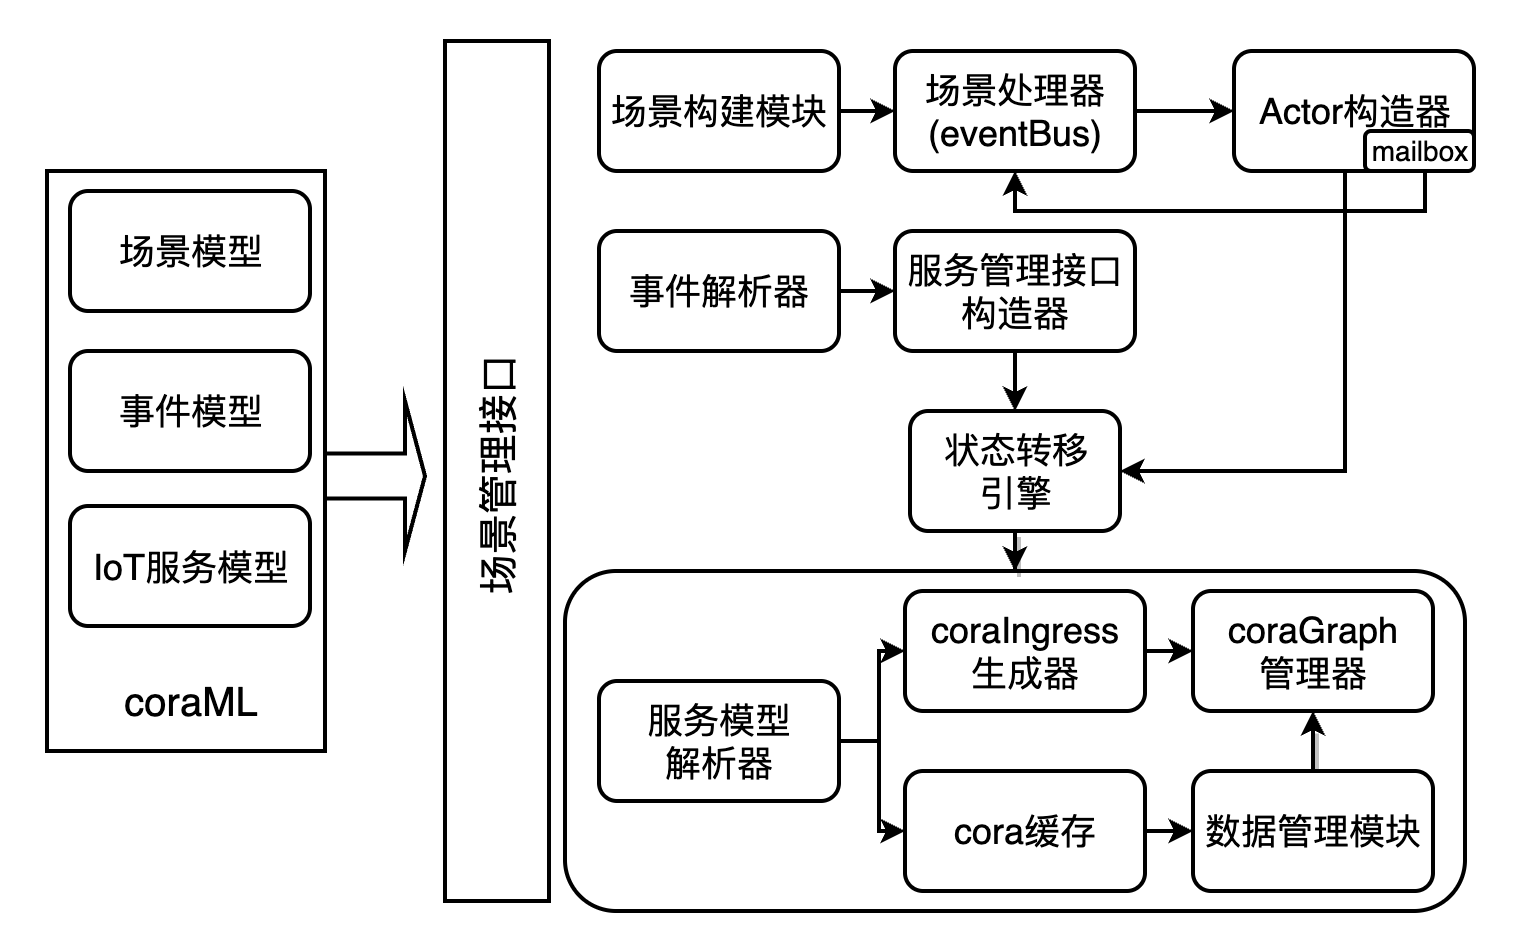
\includegraphics[width=\textwidth]{figure/4-cora/architecture.png}
	\caption{Cora框架整体架构设计}
	\label{overview}
\end{figure}


% 按照执行流程,各个模块的功能描述如下:
% \begin{itemize}
%     \item 开发人员使用coraML分别定义IoT服务模型、事件模型和场景模型,并通过场景管理接口发送给Cora。
%     \item 对于IoT服务模型,Cora中使用服务模型解析器来解析模型,通过coraIngress生成器为IoT服务模型生成管理接口,并通过CoraGraph管理器将模型注册到coraGraph中;而对于IoT服务,数据管理模块会管理IoT服务的运行数据,cora缓存中存放了IoT服务缓存数据。
%     \item 对于事件模型,Cora使用事件解析器来解析事件,通过服务管理接口构造器将解析后的事件构造成coraIngress接口,并通过状态转移引擎将接口发送给IoT服务。
%     \item 对于场景模型,场景构建模块会解析并构建场景,并通过场景处理器来管理IoT服务之间的事件发送,Actor构造器会将场景中的IoT服务构造为一个Actor。
% \end{itemize}


\section{Actor模型}
本文期望并发场景执行时,在框架层保证场景完整性、场景有序性和场景高效性。在并发场景运行中,在框架层使用锁来解决冲突问题存在很大的风险。在场景执行中对场景整体加锁会带来阻塞问题,影响场景高效性,而对IoT服务加锁可能会产生死锁问题,影响场景完整性\cite{salvaneschi2012contexterlang}。而且使用锁来解决并发问题与上文的事件驱动的IoT服务组合模型并不匹配,因为锁模型更适用于基于流程的服务组合场景。

本文认为Actor模型适用于Cora中并发场景的执行。Actor模型(The Actor Model)\cite{agha1985actors}是MIT实验室在1973年提出的一个分布式并发编程模式,并在Erlang\cite{armstrong2010erlang},Akka\cite{vernon2015reactive}中得到广泛支持和应用。Cora中使用Actor模型可以解决以下问题:
\begin{itemize}
    \item 在并发场景中,Actor模型可以代替锁来处理冲突问题,从而解决锁带来的阻塞和死锁问题。
    \item Actor模型使用协作实体对消息作出反应,改变状态,以及相互发送信号的模型来推动整个应用系统向前发展,这与本文实现的事件驱动的IoT服务组合模型相匹配。
    \item Actor模型可以保证场景高效性。Actor是事件处理的最小单元,场景中IoT服务是执行指令的最小单元,使用Actor模型构建场景可以最大程度上减少场景阻塞时间,保证场景高效性。
\end{itemize}

因此Cora基于Actor模型设计实现了三个基本模块:模型管理模块、IoT生命周期管理模块和场景构建模块。图4-1展示了Actor模型的基本架构,Actor模型主要由Actor,Mailbox,Internal State和Event构成。
\begin{figure}
	\centering
	
\includegraphics[width=0.9\textwidth]{figure/4-cora/actor_model.png}
	\caption{Actor模型架构\cite{actordef}}
	\label{ontransact-impl}
\end{figure}

\textbf{Actor}接收消息,根据业务逻辑处理消息,也可以发送消息给其他Actor。在Cora中,模型管理模块和IoT服务生命周期管理模块对应于Actor构建。

\textbf{Mailbox}与Actor实例一一对应,存放Actor接收到的所有消息,是Actor的“邮箱”,对应于Cora中的消息管理模块。

\textbf{Internal State}是Actor的内部业务逻辑,对应IoT服务的状态转移模型,通过Cora中的状态转移引擎实现。

\textbf{Event}是Actor之间的传输协议,对应于Cora中的事件。

\section{模型管理}
上文定义的IoT服务组合模型需要Cora来进行模型解释,因此模型管理模块的工作就是解析并管理上文的IoT服务组合模型。Cora实现了模型解析器来解析coraML定义的IoT服务组合模型,并分别组织管理IoT服务模型和场景模型。

\subsection{模型解析}
Cora中基于ANTLR实现coraML的模型解析器。ANTLR\cite{antlr}是一个开源的解析器生成器,用于读取、处理、执行或者翻译结构化文本或二进制文件。ANTLR广泛应用于构建语言、工具和框架,例如,Hibernate使用ANTLR来解析和处理HQL查询语句。从语法中,ANTLR可以生成一个可以构建和遍历解析树的解析器。

coraML基于JSON构建,而ANTLR支持JSON解析器的生成,所以Cora中使用ANTLR来生成JSONParser和JSONLexerJSONLexer可以支持String类型的模型描述到JSON实例的构建,JSONParser可以支持JSON实例的解析。但是ANTLR生成的JSONParser的ObjContext中只存储了一棵token组成的解析树,token中描述了叶子节点的属性类型和属性值等信息,所以需要对解析树进行遍历来得到最终结果。考虑到JSON语法本身的通用性,Cora中构建了JsonAST和JsonArray(JsonAST列表)两种中间类型,IoT服务模型,场景模型等可以从中间类型构建得到。代码4.1展示了JsonAST的成员变量和成员方法信息,parseJSON()方法会将输入的String实例构建成一个解析树,基于JSONParser深度优先遍历解析树,便可得到具体的JsonAST实例。

\begin{lstlisting}[caption={JsonAST类型},label={lst:JsonAST},language=java,basicstyle=\footnotesize]
public class JsonAST{
    private Map<String,Object> map; //map中存放树的每一层的节点信息
    
    protected JsonAST(JSONParser.ObjContext objCtx){...}
    
    public JsonAST getJSONAST(String key){...} 
    
    public static JsonAST parseJSON(String text){...} 
}
\end{lstlisting}

基于JsonAST和JsonArray,Cora中定义了CoraParser来实现模型解析。代码4.2展示了CoraParser中的接口信息。可以看到对于上文IoT服务组合模型中的各个模型,CoraParser都提供了相应的接口实现,这些接口实现的基本流程是一致的:对于输入的String类型,先调用isVaild()方法判断coraML语法的合法性;若coraML语法合法,则调用JsonAST的parseJSON()方法将String构建成中间类型JsonAST,最后基于中间类型JsonAST构建具体的各类模型实例。
\begin{lstlisting}[caption={CoraParser接口信息},label={lst:coraParser_interface},language=java,basicstyle=\footnotesize]
public interface CoraParser{
    CoraNode parsefieldSchema(String fieldSchema); //解析设备属性模型
    
    FSM parseFSM(String fsm);  //解析状态转移模型
    
    Context parseContext(String context);  //解析场景模型
    
    Event parseEvent(String event);  //解析事件模型
    
    boolean isVaild(String schema);  //判断coraML语法的合法性
}
\end{lstlisting}

需要注意的是,考虑到框架的扩展性和灵活性,开发人员可以自定义DSL或使用其他的描述语言(如xml,yaml等)来为IoT服务建模,然后继承CoraParser,基于ANTLR构建特定的语法解析器进行适配,这也是Cora使用ANTLR的原因之一。

\subsection{IoT服务模型管理}
Cora中构建了实体关系模型\textbf{CoraGraph}来统一管理平台中的IoT服务模型。图4-2展示了CoraGraph的整体架构,CoraGraph由ModelGraph和Ingress构成,用户定义的IoT服务模型会被解析为CoraNode存入ModelGraph中,ModelGraph可以通过关系型数据库或文档型数据库存储管理。CoraNode描述了IoT服务的设备模型,CoraIngress与CoraNode一一对应,代表每个IoT服务模型的可访问接口信息。考虑到IoT服务组合场景中IoT服务之间因为相互交互而存在的关联关系,实体关系模型的方式提供了极大的灵活性,并且能够有效处理模型之间的复杂关系。Cora用邻接表的形式来构建CoraGraph,CoraGraph由CoraNode列表和CoraIngress列表构成:

\textbf{CoraNode}以图节点的形式表示CoraGraph中的IoT服务模型,描述了IoT服务模型的所有信息,包括CoraNode设备属性模型,状态转移属性和一些模型实例的信息,例如代码4.1和代码4.2中定义的空气净化器服务的设备属性模型和状态转移模型都会存放在空气净化器服务模型对应的CoraNode中。需要注意的是,每个CoraNode都会保存其关联的CoraNode信息,即图模型中每个节点的入度信息,例如洗衣机服务模型可以关联烘干机服务模型。代码4.3描述了CoraNode类型的信息。

\begin{figure}
	\centering
	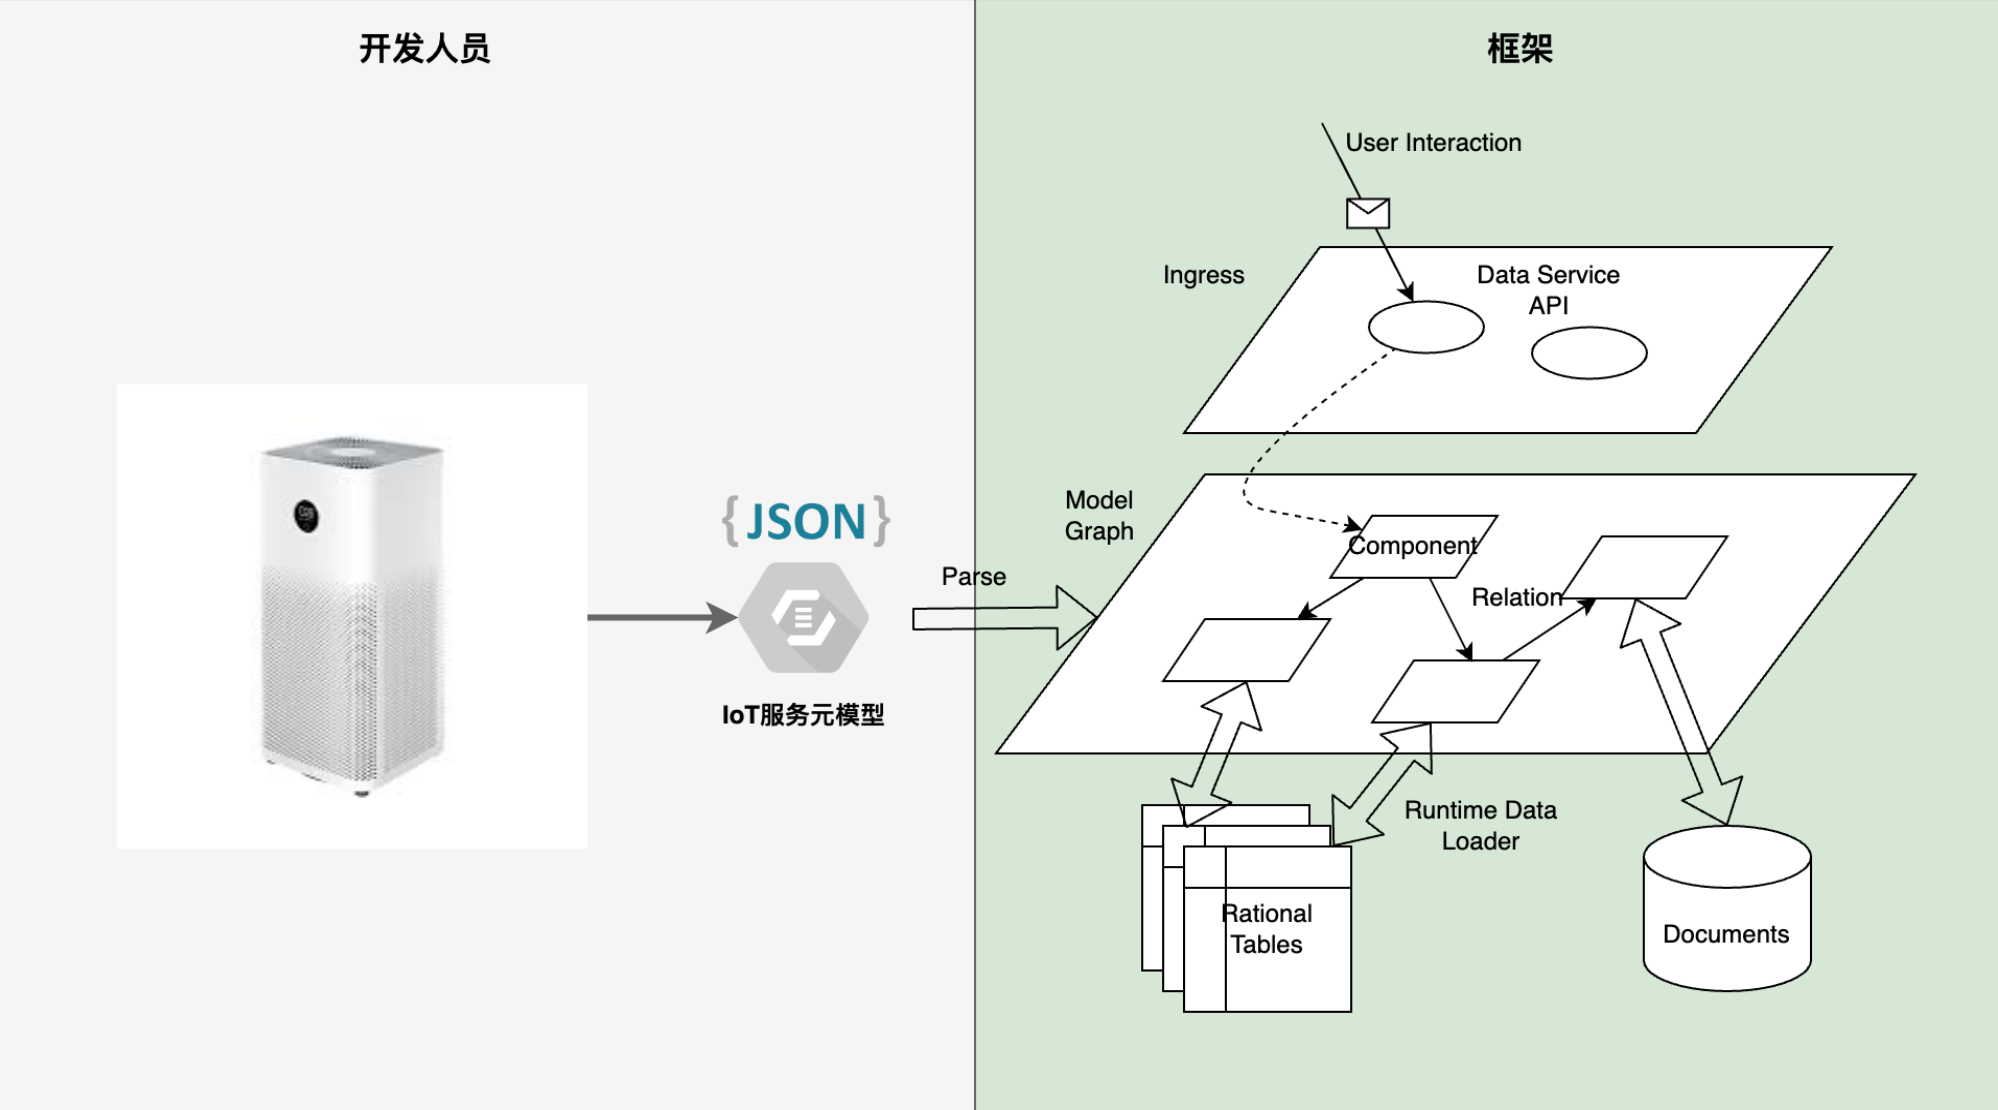
\includegraphics[width=1.0\textwidth]{figure/4-cora/CoraGraph.png}
	\caption{CoraGraph架构}
	\label{ontransact-impl}
\end{figure}

\begin{lstlisting}[caption={CoraNode类型信息},label={lst:CoraNode},language=java,basicstyle=\footnotesize]
public class CoraNode {
    ......
    private Definition definition;     //模型定义
    private Map<String,Type> typeMap;  //设备属性模型
    private FSM fsm;                   //状态转移模型
    private List<CoraNode> children;   // 关联的CoraNode列表
    ......
}
\end{lstlisting}

\textbf{CoraIngress}与CoraNode一一对应,代表每个IoT服务模型的可访问接口信息。CoraIngress随着CoraNode的注册由框架生成,CoraIngress的作用是给用户提供管理模型及模型实例的生命周期的方式,除了标准统一的生命周期管理接口,用户也可以自定义实现CoraIngress。代码4.4描述了CoraIngress类型的信息。
\begin{lstlisting}[caption={CoraIngress类型信息},label={lst:CoraIngress},language=java,basicstyle=\footnotesize]
public class CoraIngress {
    private String modelId;     //模型唯一标识
    private List<ImmutablePair<String,Ingress>> ingressList; //可访问接口列表
    ......
}
\end{lstlisting}

CoraGraph默认持久化在数据存储模块。在项目启动时,Cora会从数据存储模块中拉取所有的IoT服务模型信息,解析生成全局的CoraGraph实例进行管理,Cora用邻接表来构建CoraGraph。在项目运行时,当开发人员注册新的IoT服务模型时,CoraParser会解析生成CoraNode,并将CoraNode填入CoraGraph中,并为CoraNode生成CoraIngress;然后用户便可通过CoraIngress根据CoraNode中的IoT服务模型注册IoT服务实例,管理该IoT服务实例。

\subsection{场景模型管理}
Cora中用\textbf{Context}类型来描述场景,对应于服务组合模型中的场景模型。场景信息默认持久化在数据存储模型,在项目启动时,Cora会从数据存储模块中拉取所有的场景信息,完成场景初始化构建,例如Cora启动时,会拉取并解析代码3.4展示了\textit{净化空气场景}模型。代码4.5描述了Context类型的信息。
\begin{lstlisting}[caption={Context类型信息},label={lst:Context},language=java,basicstyle=\footnotesize]
public class Context{
    ......
    private List<String> actorIds;   //IoT服务实例列表
    private Map<String,Map<Pair<String,String>,ContextEvent>> onEvents; 
    private Map<String,Actor> actorMap;
}
\end{lstlisting}

总结来说,针对上文中介绍的IoT服务组合模型,Cora中的模型管理模块首先基于coraML构建了模型解析器,解析得到各种模型类型,通过实体关系模型CoraGraph统一组织管理IoT服务模型,并用Context类型来管理场景模型。



\section{IoT服务生命周期管理}
IoT服务的生命周期管理接口是场景构建的基础。开发人员通过IoT服务的生命周期管理接口来更新IoT服务的状态,根据上文,IoT服务组合实质上是一系列IoT服务的状态变更集合,因此IoT服务的生命周期管理接口是Cora进行场景构建的基础。但是一方面受限于不同的IoT服务厂商之间的技术壁垒,不同厂商的IoT服务往往不能提供统一的开发流程和服务接口,例如小米IoT开发者平台和华为IoT物联网社区提供了不同的开发流程和服务接口设计规范,不同规范的服务管理接口会阻碍服务组合逻辑的实现,在服务组合实现时会造成不必要的开发负担;另一方面,基于MDD和上文IoT服务组合模型,开发人员只需关注于于IoT服务组合建模,服务管理接口可以由框架构建管理。

因此,Cora的IoT服务生命周期管理模块为IoT服务提供标准统一的生命周期管理接口。针对不同的IoT服务,Cora为开发人员构建生成了标准统一的IoT服务生命周期管理接口,这样开发人员便可以使用统一风格的接口进行开发,提高开发效率,也在框架层为后文的场景构建打下基础。

具体实现来看,本文基于关注点分离(SoC)原则设计实现IoT服务生命周期管理模块。图4-3展示了空气净化器服务的生命周期,可以看到空气净化器服务的完整生命周期主要包括四个部分:净化器服务创建,净化器服务状态查询,净化器服务状态转移和净化器服务下线。对应的关注点依次是净化器服务状态属性,净化器服务实时状态或历史数据,净化器服务状态转移控制器和净化器服务删除。基于SoC原则,开发人员需要关注净化器服务的功能属性和状态描述,开发人员可以通过IoT服务组合模型进行描述,而Cora需要提供净化器服务的状态管理接口和数据存储服务。具体实现来看,Cora的IoT服务生命周期管理主要分为IoT服务接口生成,IoT服务实例存储,并且框架为查询接口做了性能优化。
\begin{figure}
	\centering
	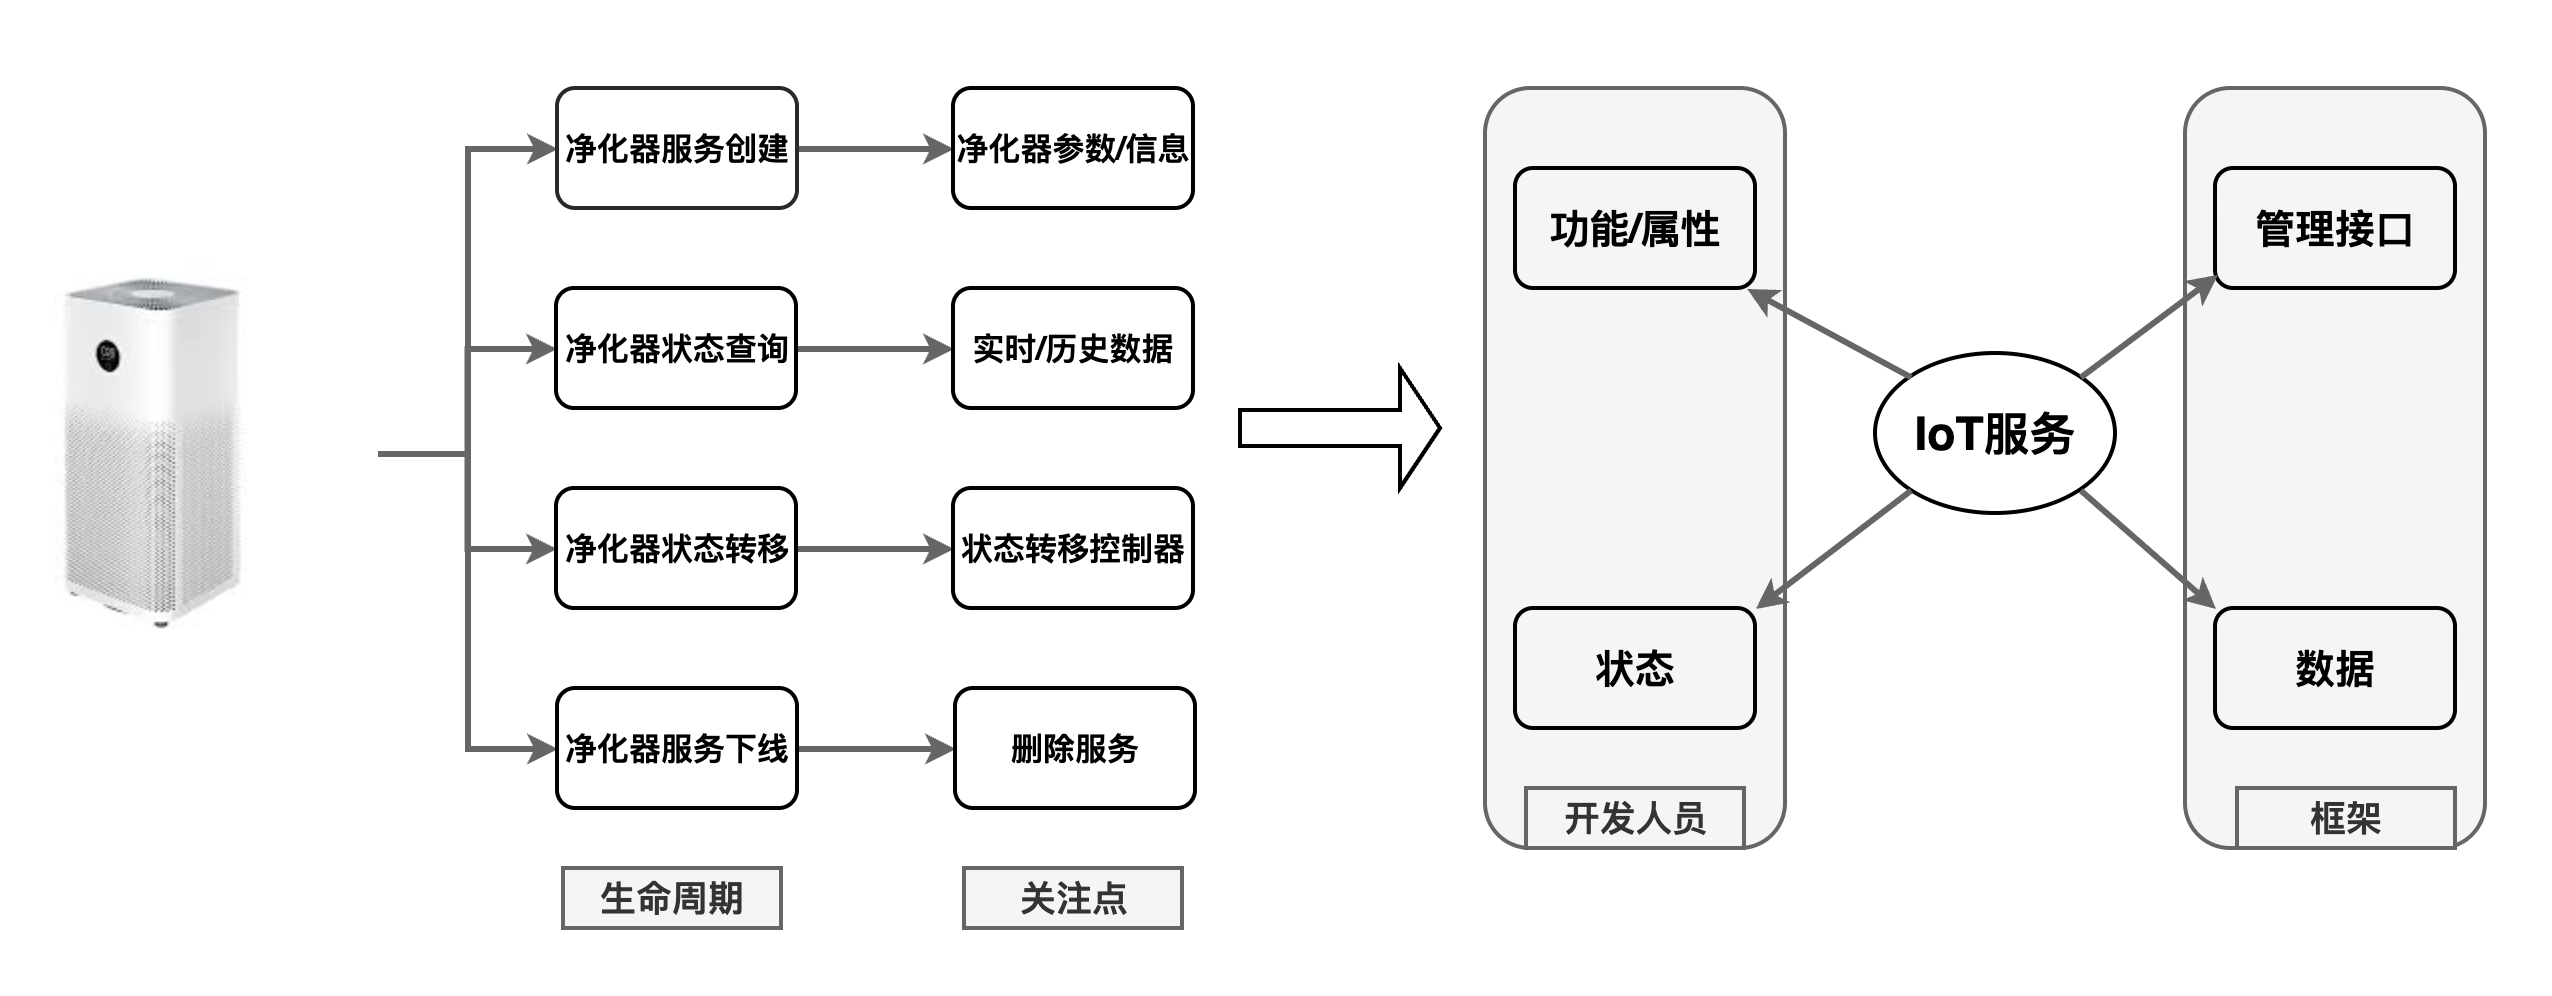
\includegraphics[width=1.0\textwidth]{figure/4-cora/airpurifier_lifecycle.png}
	\caption{空气净化器服务的生命周期}
	\label{ontransact-impl}
\end{figure}

\subsection{IoT服务接口生成}
标准统一的接口是进行高效场景构建的基础,异构的IoT服务管理接口会在Cora进行服务组合的过程中,带来很多繁琐不必要的适配负担。基于graphql-java框架,Cora采用了一种运行时接口动态生成的方式来为IoT服务生成GraphQL类型的生命周期管理接口。接口生成技术主要有静态代码生成和动态解析生成两种方式,静态代码生成主要面向系统实现,被用来代替人工编码。用户可以使用一些成熟的接口生成工具(Swagger\cite{swagger}、Retool\cite{retool}等)静态生成Restful API\cite{richardson2008restful}等主流接口。动态解析生成技术主要面向开发框架,用户在平台中创建一些运行实例,框架会为这些实例动态生成访问接口。例如数据库系统,服务治理平台等都是用动态解析生成的接口生成方式。

Cora中使用动态解析生成技术为IoT服务生成接口。相较于静态代码生成的方式,动态接口生成的方式可以减少不必要的框架代码,还可以避免系统重启的时间开销。Cora的接口生成模块主要有四部分构成:CoraRuntimeWiring,CoraTypeRegistry,CoraBuilder和CoraDataFetcher。

\paragraph{为什么使用GraphQL?}
Cora中的接口生成模块主要基于graphql-java\cite{graphqljava}框架实现。GraphQL\cite{graphql}由meta公司的前身facebook在2012年提出,近年来迅速在工业界流行起来,在学术界也收获了很大的关注,其开发生态也在迅速扩张\cite{DBLP:conf/icsoc/WitternCDBM19}。根据官方定义\cite{graphqlsdl},GraphQL是一种API查询语言,也是一种服务器端运行时,可以基于用户定义的类型系统为数据执行查询。GraphQL不依赖于任何特定的数据库或存储引擎,而是由用户现有的代码和数据支持。本文认为GraphQL的核心概念是用图的方式来组织数据模型,主要由两部分构成,首先是概念层,或者说模型层,官方定义GraphQL是一种API查询语言,但是随着应用场景的扩展,GraphQL不仅仅局限于查询,也支持数据更新(Mutation)等,因此很多工作也开始将GraphQL与Restful API进行对比,所以本文认为GraphQL是一种API模型;此外GraphQL除了是一种API模型之外,它也是一个执行引擎,执行引擎语言不限,可以和各种后端服务绑定使用。facebook官方实现了javaScript版本的graphql-js,此外开源社区还有graphql-java,graphql-go,graphql-ruby等多种语言实现。

Cora中采用GraphQL API主要考虑了GraphQL的特性和IoT服务组合场景的特点。
\begin{itemize}
    \item GraphQL用图的方式来组织数据模型,Cora用CoraGraph来统一管理IoT服务模型,两者相互统一。在进行接口生成时,两者底层模型的高度匹配带来了很大的开发便利,同时也减少了大量的工作量,这也是本文采用GraphQL的直接原因。
    \item 相较于Restful API,GraphQL具有减少网络通信开销,减少过度获取属性(Overfetching)等优势。
    \item GraphQL查询语言支持关联查询,而Restful API只支持单个资源信息的获取,GraphQL在IoT服务之间的关联状态查询方面更有优势。
\end{itemize}

\begin{figure}
	\centering
	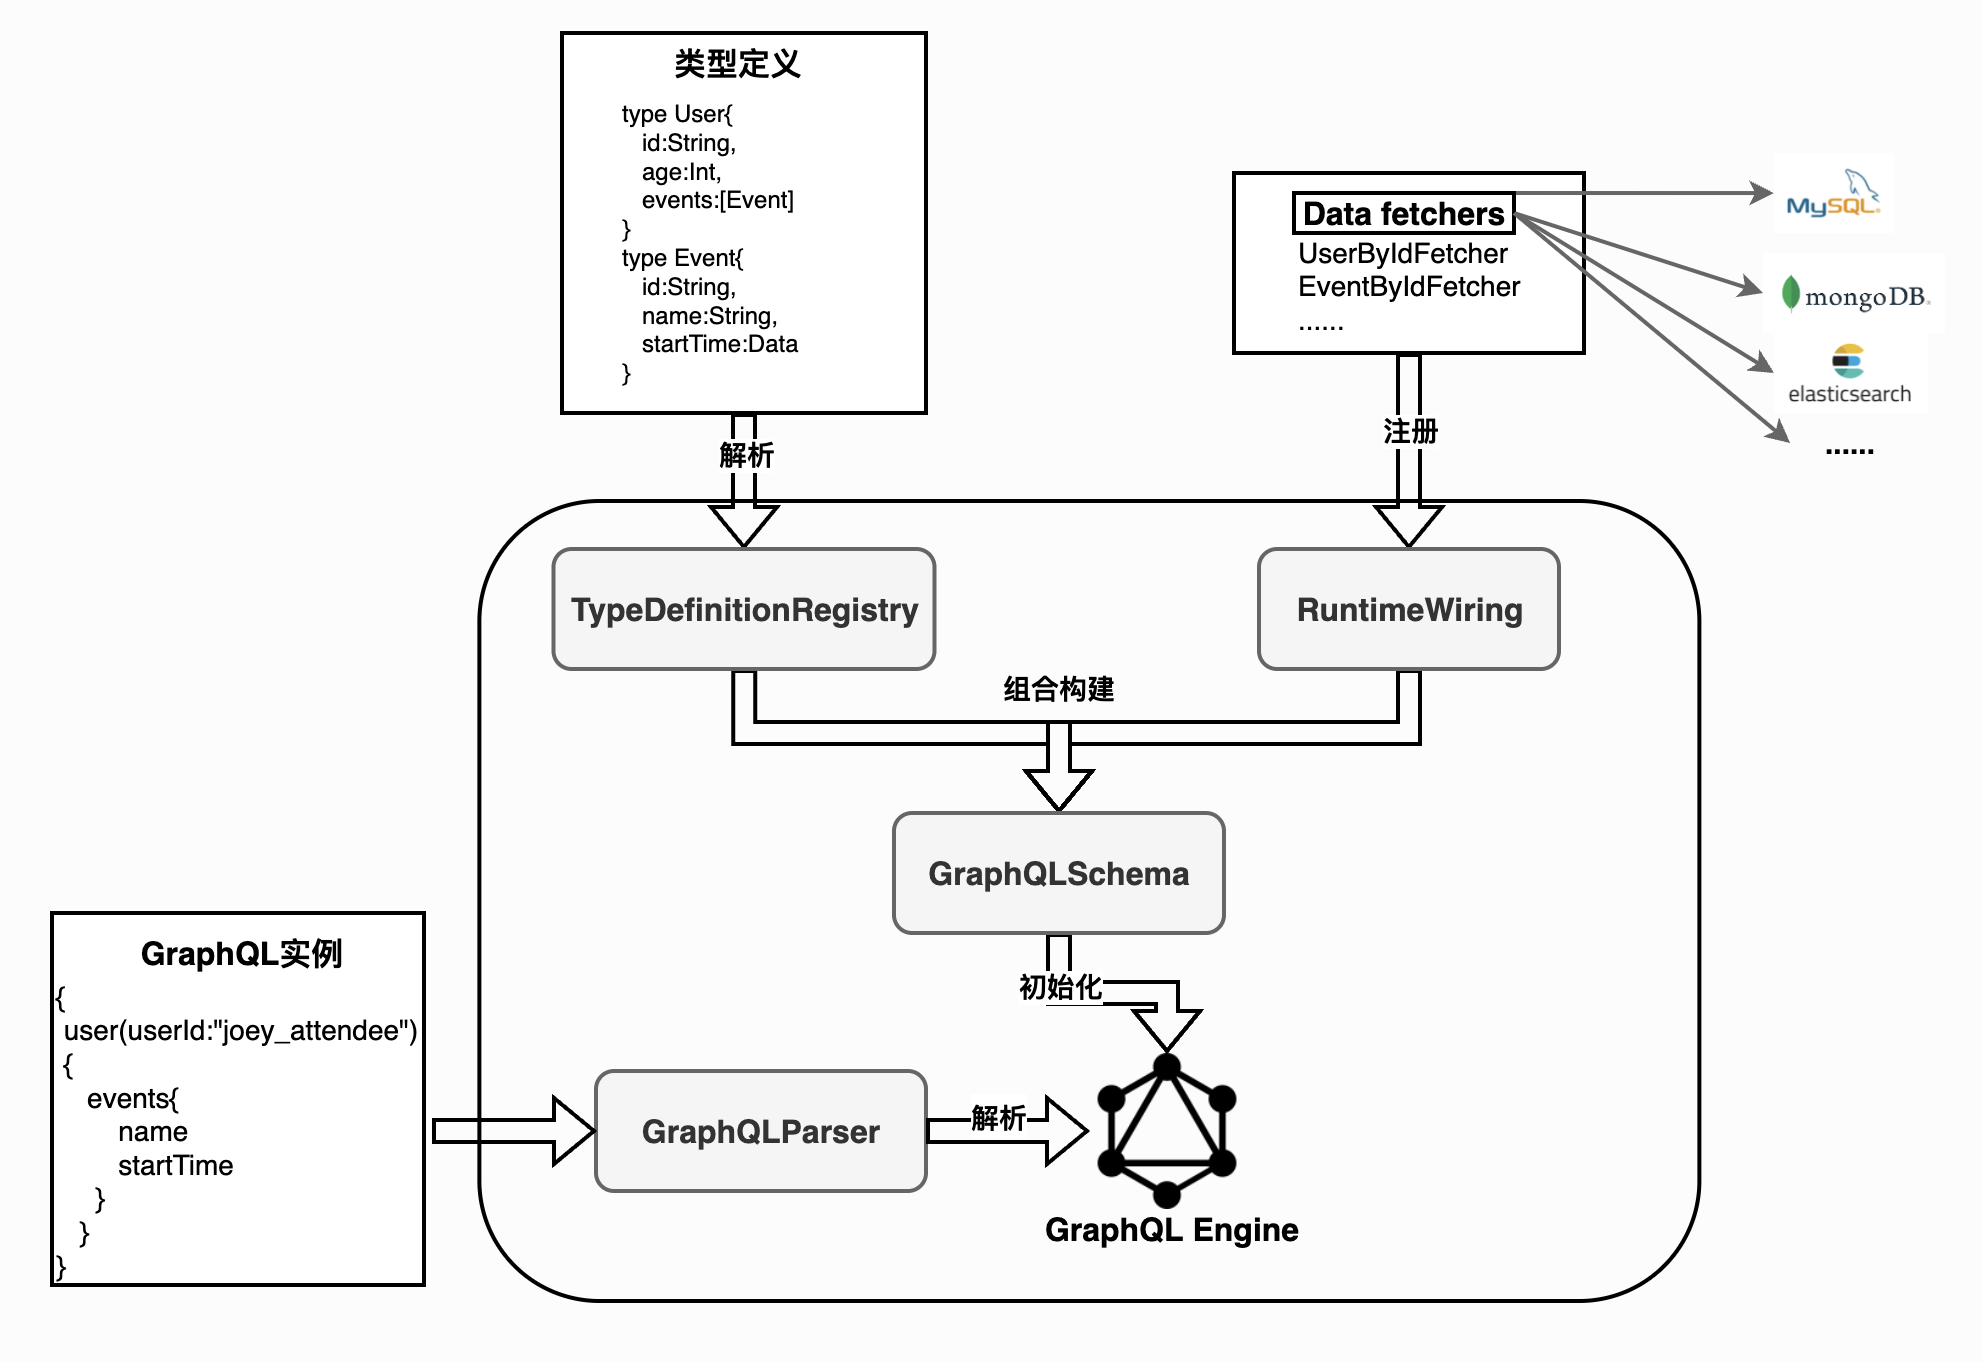
\includegraphics[width=1.0\textwidth]{figure/4-cora/graphql_java_architecture.png}
	\caption{基于graphql-java的开发流程}
	\label{ontransact-impl}
\end{figure}

原生的graphql-java框架无法支持接口生成,因此Cora中基于graphql-java框架进行了部分重构,实现了接口生成模块。为了更好地阐述本模块工作,图4-4展示了基于graphql-java框架的系统开发流程。首先用户需要基于GraphQL SDL(Schema Definition Language)\cite{graphqlsdl}定义接口类型和模型类型,接口类型主要包括查询类型(Query)和更改类型(Mutation)两种,其中定义了GraphQL API信息。graphql-java框架会将模型注册到TypeDefinitionRegistry中,TypeDefinitionRegistry中存储了所有的模型定义信息,与CoraGraph作用类似;此外用户需要实现自定义的DataFetcher来连接各种类型的数据库或存储引擎;graphql-java框架会将所有的DataFetcher接口注册到RuntimeWiring中,RuntimeWiring中主要存储了接口描述和DataFetcher接口的字典,针对不同类型的GraphQL查询实例中的数据模型,框架会根据RuntimeWiring定位到具体的DataFetcher来进行数据操作;RuntimeWiring和TypeDefinitionRegistry共同构建完成graphqlEngine运行时,最后用户就可以发送GraphQL API给graphqlEngine执行具体的操作。

\paragraph{接口生成模块}
原生的graphql-java框架无法支持接口生成,其原因如下:1)GraphQL SDL无法支持coraML的模型语义2)graphql-java不支持动态管理数据模型;3)graphql-java不支持接口生成。因此针对上述问题,Cora基于graphql-java框架,主要进行了以下工作: 1)适配并扩展了graphql-java的模型管理,使其支持IoT服务组合模型管理;2)动态维护并更新graphql-java的数据模型;3)基于IoT服务模型,支持动态接口生成。


具体实现来看,接口生成模块的核心是在运行时基于CoraGraph构建graphqlEngine,为IoT服务生成GraphQL API。基于graphql-java的系统开发流程,用户需要预先用GraphQL SDL定义模型,还需要编码实现DataFetcher接口,最后调用graph-java框架的API构建运行时系统,在Cora中这几部分在接口生成模块中需要动态生成。

具体实现思路是,首先将CoraGraph中所有CoraNode的设备属性模型注册到TypeDefinitionRegistry中,并基于静态模板生成查询类型(Query)和更改类型(Mutation),所以Cora中构建了CoraTypeRegistry动态维护TypeDefinitionRegistry;此外Cora中构建了统一的CoraDataFetcher,所有的IoT服务都会匹配到CoraDataFetcher,换言之所有IoT服务实例的更改查询操作都可以通过CoraDataFetcher进行,并且实现了CoraRuntimeWiring来动态维护RuntimeWiring;最后Cora构建了CoraBuilder来动态构建graphqlEngine。

\textbf{CoraTypeRegistry}:
CoraTypeRegistry的作用是将CoraGraph中所有的CoraNode的设备属性模型和生命周期管理接口注册到graphql-java框架的TypeDefinitionRegistry中去。因为按照graphql-java的实现,类型包括两部分组成,一部分是模型类型,也就是ObjectType,对应于CoraNode的设备属性模型;另一部分是接口类型,也就是开发人员可以使用的更改查询接口类型,对应于Cora中IoT服务的生命周期管理接口。CoraTypeRegistry中主要有成员变量typeDefinitionMap,fieldDefinitionListInQuery和typeDefinitionRegistry,typeDefinitionRegistry是graphql-java的实例。typeDefinitionMap维护平台中所有CoraNode的设备属性类型,fieldDefinitionListInQuery用来维护所有CoraNode的查询接口类型。随着CoraNode中的属性信息更新,Cora会更新typeDefinitionMap和fieldDefinitionListInQuery,进而更新typeDefinitionRegistry。

当开发人员新建或者修改平台中的CoraNode时,CoraTypeRegistry首先会从CoraNode中获取typeMap和inputMap等属性信息,更新相应的属性描述和接口描述,然后更新typeDefinitionMap和fieldDefinitionListInQuery,最后调用buildTypeRegistry()方法更新typeDefinitionRegistry。代码4.6展示了CoraTypeRegistry的部分类型信息。
\begin{lstlisting}[caption={CoraTypeRegistry类型信息},label={lst:CoraTypeRegistry},language=java,basicstyle=\footnotesize]
public class CoraTypeRegistry {
    private final TypeDefinitionRegistry typeDefinitionRegistry;    
    
    private static Map<String,Map<String,Type>> typeDefinitionsMap; 
    
    private final List<FieldDefinition> fieldDefinitionListInQuery;              
    ......
}
\end{lstlisting}

\textbf{CoraDataFetcher}:
CoraDataFetcher的作用是数据获取网关(GateWay),CoraDataFetcher与数据存储层交互,将不同CoraNode的数据管理接口统一化。不同的CoraNode有不同的“增删改查”接口,但是都会通过CoraDataFectcher与数据存储模块交互,CoraDataFetcher可以从dataFetcherEnvironment中获取接口信息,并在CoraDataFetcher中统一整合,调用数据存储模块的CoraRepository实现与数据库的统一交互。

以创建CoraNode实例为例,CoraDataFetcher中注入CoraRepository实例,在getCreator()方法的dataFetcherEnvironment参数中获取需要创建的数据和类型信息,通过CoraRepository的createNodeInstance()方法将实例持久化到数据库中。代码4.7展示了CoraDataFetcher中的getCreator()方法。
\begin{lstlisting}[caption={CoraDataFetcher中的getCreator()方法},label={lst:getCreator()},language=java,basicstyle=\footnotesize]
{
    ......
    @Override
    public DataFetcher<T> getCreator(){
        return dataFetcherEnvironment -> {
            ......
            return coraRepository.createNodeInstance(nodeType,data);
        };
    }
}
\end{lstlisting}

\textbf{CoraRuntimeWiring}:
CoraRuntimeWiring的作用是维护生成的接口类型与DataFetcher实例字典。按照graphql-java框架的设计,每个接口类型都需要与特定的DataFetcher匹配,这样框架在执行查询语句时都可以调用相应的DataFetcher。按照上文所示,Cora提供了统一的DataFetcher,即Cora中只有全局单例的CoraDataFetcher实例,所有CoraNode的查询类型都与全局单例的CoraDataFetcher对应,Cora在执行不同CoraNode生成的查询语句时都调用同一个DataFetcher实例。这样设计可行的原因是:不同于一些大数据场景,智能家居场景下的IoT服务组合不是一个数据修改高频的场景,但是大量的IoT服务模型在Cora中会生成大量的CoraNode,从而生成大量的DataFetcher实例,所以在性能影响不大的情况下,这样设计可以大量减少运行时的DataFetcher实例,减少内存开销。

具体到实现,CoraRuntimeWiring中注册了nodeInstanceFetcher,nodeInstanceListFetcher,nodeInstanceConstructor等DataFetcher实例,当注册新的CoraNode时,根据CoraNode生成对应的增删改查类型,将类型与相应的DataFetcher绑定,注册到RuntimeWiring实例中。代码4.8描述了CoraRuntimeWiring部分类型信息。
\begin{lstlisting}[caption={CoraRuntimeWiring类型信息},label={lst:CoraRuntimeWiring},language=java,basicstyle=\footnotesize]
public class CoraRuntimeWiring {
    private final RuntimeWiring runtimeWiring;    
    
    private final DataFetcher nodeInstanceFetcher;
    
    private final DataFetcher nodeInstanceListFetcher;
    
    private final DataFetcher nodeInstanceConstructor;
    ......
}
\end{lstlisting}

\textbf{CoraBuilder}:
CoraBuilder的作用是根据生成的RuntimeWiring实例和TypeDefinitionRegistry实例生成graphqlEngine实例。根据上文,Cora基于CoraNode构建完成CoraRuntimeWiring和CoraTypeRegistry,利用graphql-java框架中提供的build()方法,可以生成graphqlEngine实例,用户的“增删改查”接口便可通过graphqlEngine执行。此外graphqlEngine的初始化以及graphqlEngine的实时更新也在CoraBuilder中实现。当Cora启动时,会扫描一遍数据库中的模型定义表,遍历该表,构建CoraGraph,将所有的CoraNode类型注册到graphqlEngine中,当发生CoraNode的更新时,CoraBuilder也会调用相应的增删改查方法,实时重新构建graphqlEngine实例。代码4.9描述了CoraBuilder中的createGraphQL()方法。
\begin{lstlisting}[caption={CoraBuilder中的createGraphQL()方法},label={lst:createGraphQL()},language=java,basicstyle=\footnotesize]
{
    ......
    public GraphQL createGraphQL(){
        ......
        coraNodes.forEach( coraNode -> {
            ......
            CoraGraph.merge(coraNode);
        });
    }
    coraTypeRegistry.buildTypeRegistry();
    coraRuntimeWIring.buildRuntimeWiring();
    this.graphQLSchema = schemaGenerator.makeExecutableSchema(
            coraTypeRegistry.getTypeDefinitionRegistry()
            , coraRuntimeWiring.getRuntimeWiring());
    return newGraphQL(graphQLSchema).build();
}
\end{lstlisting}
\paragraph{接口示例}
本文以\textit{净化空气场景}中的净化器服务为例展示接口生成模块为IoT服务生成的GraphQL风格的各种类型接口。
\begin{itemize}
  \item [1)] 
  创建空气净化器服务,并关联一个传感器服务实例:
  \begin{lstlisting}[language=json,basicstyle=\footnotesize]
{
    create_airPurifier(data:{
        purifierId:"purifier_1",
        sensorId:"61988226336552", //关联传感器服务
        brand:"brand_A",
        speed:100,
        isRunning:true,
        state:"Running"
    }){
        _id  //主键
        brand
    }
}
  \end{lstlisting}
  \item [2)]
  删除空气净化器服务:
   \begin{lstlisting}[language=json,basicstyle=\footnotesize] 
{
    delete_airPurifier(_id:"619892261336552"){
         deleteResult
    }
}
  \end{lstlisting}
  \item [3)]
  根据id查询空气净化器服务实例,并关联查询传感器服务状态:
  \begin{lstlisting}[language=json,basicstyle=\footnotesize] 
{
    query_airPurifier(_id:"619892261336552"){
        sensor{
            _id
            temp
        }
        speed
    }
}
   \end{lstlisting}
  \item [4)]
  查询空气净化器服务实例列表,并关联查询传感器服务状态:
   \begin{lstlisting}[language=json,basicstyle=\footnotesize] 
{
    query_airPurifier_list{
        sensor{
            temp
        }
        speed
    }
}
   \end{lstlisting}
  \item [5)]
  根据筛选条件(\_and、\_or)查询空气净化器服务实例列表:
  \begin{lstlisting}[language=json,basicstyle=\footnotesize] 
//单个筛选条件
{
    query_airPurifier_list(where:{
        speed:{
            _eq:100
        }
    }){
        _id
        brand
        speed
    }
}
//_and || _or
{
    query_airPurifier_list(where:{
        _and|_or:[
            {speed:{_eq:100}},
            {brand:{_eq:"brand_A"}}
        ]
    }){
        _id
        brand
        speed
    }
}
\end{lstlisting}
\end{itemize}

\subsection{IoT服务实例存储}
考虑到框架的扩展性和灵活性,Cora支持不同类型的数据库服务和存储服务,开发人员可以灵活适配所需的存储服务。一般来说,不同的数据库服务有特定的client库,为了适配不同的client库,Cora封装了CoraRepository<T>接口,开发人员可以继承CoraRepository<T>接口来实现相应的方法。Cora框架中实现了文档型数据库Mongodb和关系型数据库Mysql两种CoraRepository<T>。考虑到IoT服务数据多是以JSON形式存储表示,Cora默认采用Mongodb作为数据存储支持。

\subsection{性能优化}
Cora中IoT服务生命周期管理模块的性能优化主要集中在对GraphQL的查询优化,主要包括查询语句过滤和图缓存优化两部分。相较于Restful API,GraphQL具有减少网络通信开销,减少过度获取属性和便于前后端连通等优势,但是查询的灵活性也带来了相应的开销代价,目前最受学术界和工业界广泛关注的问题就是GraphQL嵌套查询带来的N+1问题\cite{hartig2018semantics},Cora中通过查询语句过滤和图缓存优化两种方式对N+1问题做了优化。

\paragraph{N+1问题}
在Restful API的设计理念中,每个资源都代表一个实体,所以每个Restful API都是获取某个资源的信息,当资源与资源之间存在关联关系时,需要依次访问不同资源的Restful API来获取相应的资源信息,这样的方式会产生多次的网络通信,并且获取的完整的资源信息集合往往大于用户所需的部分资源信息\cite{brito2020rest}。GraphQL解决了Restful API存在的问题,它的查询语法更为灵活,用户只需声明所需查询的资源属性,并且支持嵌套语法描述,这样就减少了网络通信开销,将多次网络通信合并为单次网络通信。并且GraphQL按需获取资源属性,减少了过度获取资源带来的传输负载。但是如果将用户对资源的一次获取等价于一次对数据库的查询操作,如图4-5所示,随着嵌套的层数增加,对数据库的查询次数也会呈指数级上升,查询结果的大小也会呈指数级上升,这样对服务端的压力也是呈指数级上升的,极端情况下会导致服务端不可用的问题,这就是
GraphQL的N+1问题。
\begin{figure}
	\centering
	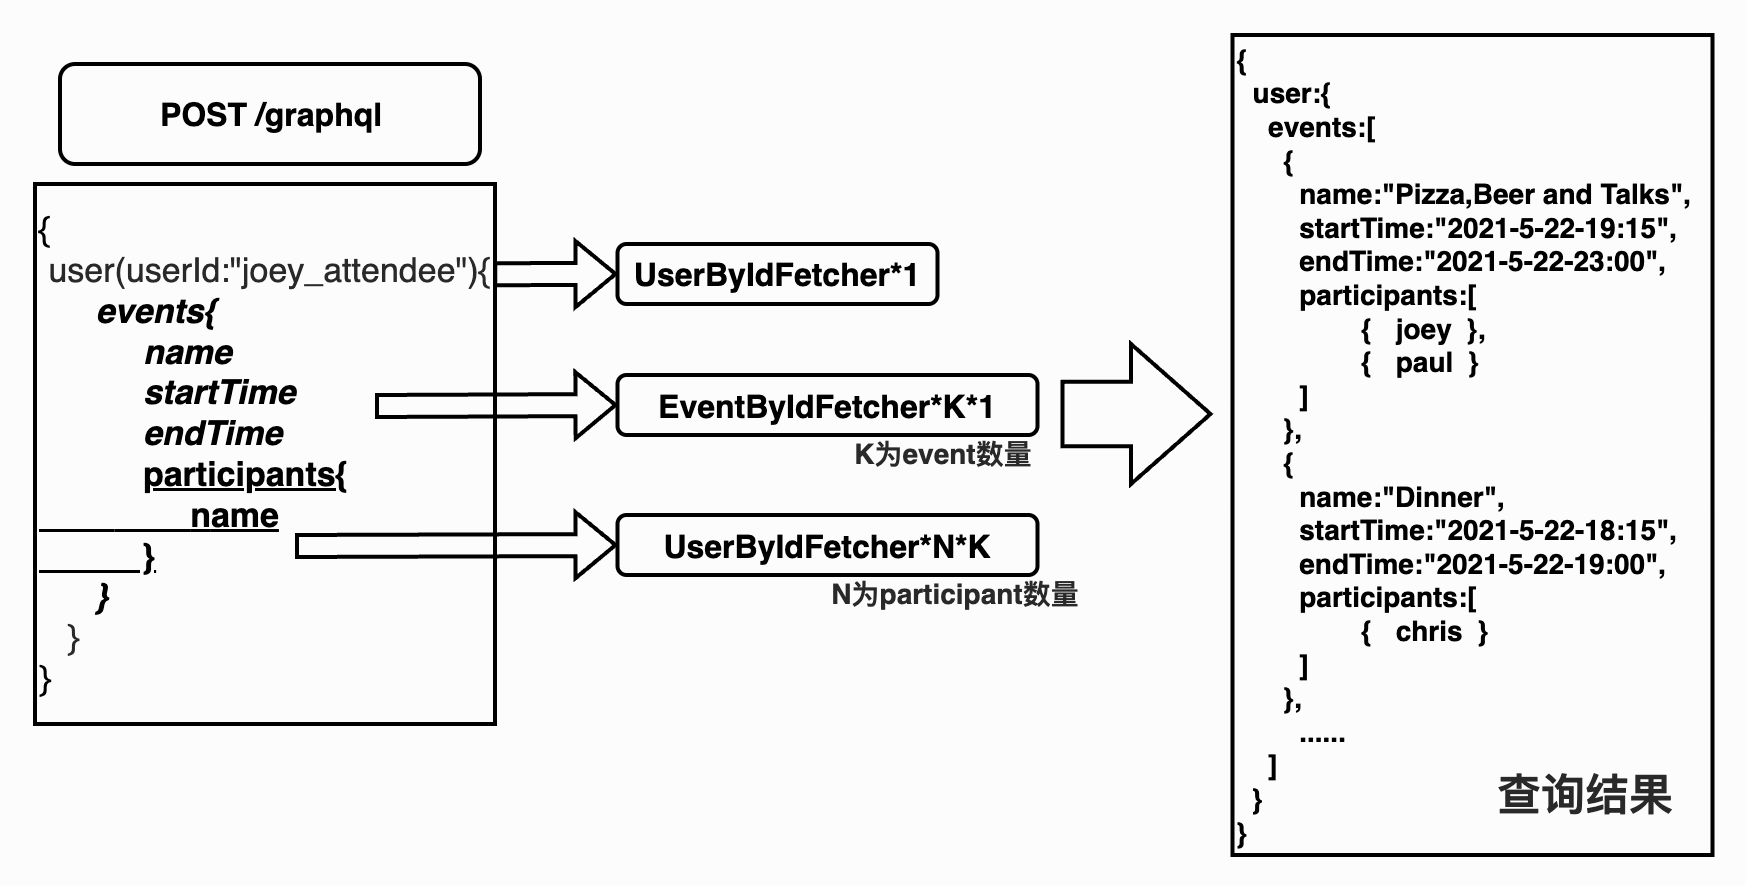
\includegraphics[width=1\textwidth]{figure/4-cora/graphql_N+1.png}
	\caption{GraphQL查询的N+1问题}
	\label{ontransact-impl}
\end{figure}

\paragraph{相关工作}
N+1问题是GraphQL应用的热点问题,在学术界和工业界引起了广泛关注,本文选择了以下具有代表性的研究工作。
\begin{itemize}
    \item \textbf{开销评估}:
    开销评估的核心是在GraphQL查询语句进入graphqlEngine之前,通过静态分析查询语句的层次结构信息,从而预估查询语句的实际开销情况,目标是过滤开销过大的查询语句,从而避免服务端执行开销过大的查询语句。Alan Cha等人\cite{cha2020principled}通过静态分析,深度学习\cite{mavroudeas2021learning}等方式进行GraphQL开销分析方面的工作,并取得了一定的效果。
    \item \textbf{查询语句缓存}:
    每条GraphQL查询语句在进入graphEngine之前都需要解析,查询语句缓存的核心是通过缓存查询语句的方式来减少重复解析相同查询语句的时间\cite{reagroup}。目前graphql-java框架中已经集成了相关接口,但是N+1问题的主要开销还是数据库的过量查询开销,查询语句缓存可以减少执行开销,但是对解决N+1问题效果不明显。
    \item \textbf{基于开发场景优化}:
    基于开发场景优化就是用户在具体应用开发时根据具体场景进行优化,这种优化方式存在很大的灵活性,且与开发的任务逻辑相耦合,无法集成到通用框架中,其主要的目标就是减少对数据库的查询访问。主要的方法包括利用数据库的批量处理接口来整合大量相似的单个查询操作,减少对数据库的访问;应用中添加数据缓存层,从而减少对数据库的访问。主要的工作包括shopify的graphql-batch\cite{graphqlbatch},graphql-js的DataLoader\cite{dataloader}等。
\end{itemize}

\paragraph{Cora查询优化}
为了解决Cora中的N+1问题,Cora采用了查询语句过滤和图缓存优化相结合的方式实现。

\textbf{查询语句过滤} 主要借鉴了GraphQL开销分析相关的工作,主要工作是解析分析查询语句的嵌套层数,并通过嵌套层数来过滤开销过大的查询语句。嵌套层数是影响查询语句执行效率的关键,查询语句的执行开销随着嵌套层数的增加而指数级增长,因此查询语句的实际执行时间和返回结果的实际空间大小很大程度上也取决于嵌套层数。因此Cora在查询语句解析过程中,统计其嵌套层数和每层的查询接口类型,对于嵌套层数大于K(K>10被认为是不可接受的嵌套层数),且列表查询数量大于M(M>5)的查询语句,会进行过滤,并向用户回复异常信息。

% \[ T(n)= \sum\limits_{n = 1}^n  {({M/1}*T(n-1))}  \]
% \[ S(n)= \sum\limits_{n = 1}^n  {({M/1}*T(n-1)*k/N)}  \]

\textbf{图缓存优化} 的核心是基于CoraGraph,在CoraNode上为对应的实例构建查询语句路径和对应查询实例实体的字典。传统的缓存方法是在缓存介质中存储一定数量的查询语句和查询结果的字典,但是这种方式在GraphQL场景中缓存命中率不高,因为GraphQL查询语句描述会细化到需要查询的具体属性的声明,不同的查询语句可能对应于相同的查询语句结构,如图4-6所示,虽然查询语句结构一致,只是最后查询结果的字段有所差异,但是这会在缓存中占用两个缓存槽,从而带来重复缓存的问题,在GraphQL的场景下,这种传统的实现方式显然也会带来缓存命中率不高的问题。并且当缓存中数据发生更改时,因为缺乏详细的查询语句结构信息,如果采用最暴力的方式清空所有的缓存,那么显然会影响缓存命中率,如果遍历缓存字典,分析查询语句结构,从而寻找受数据更新影响的缓存槽并且丢弃,这种方式虽然不会影响缓存命中率,但是这种遍历分析的方式时间开销很大,也并不适用。因此传统的缓存方法在GraphQL的场景下并不适用。
\begin{figure}
	\centering
	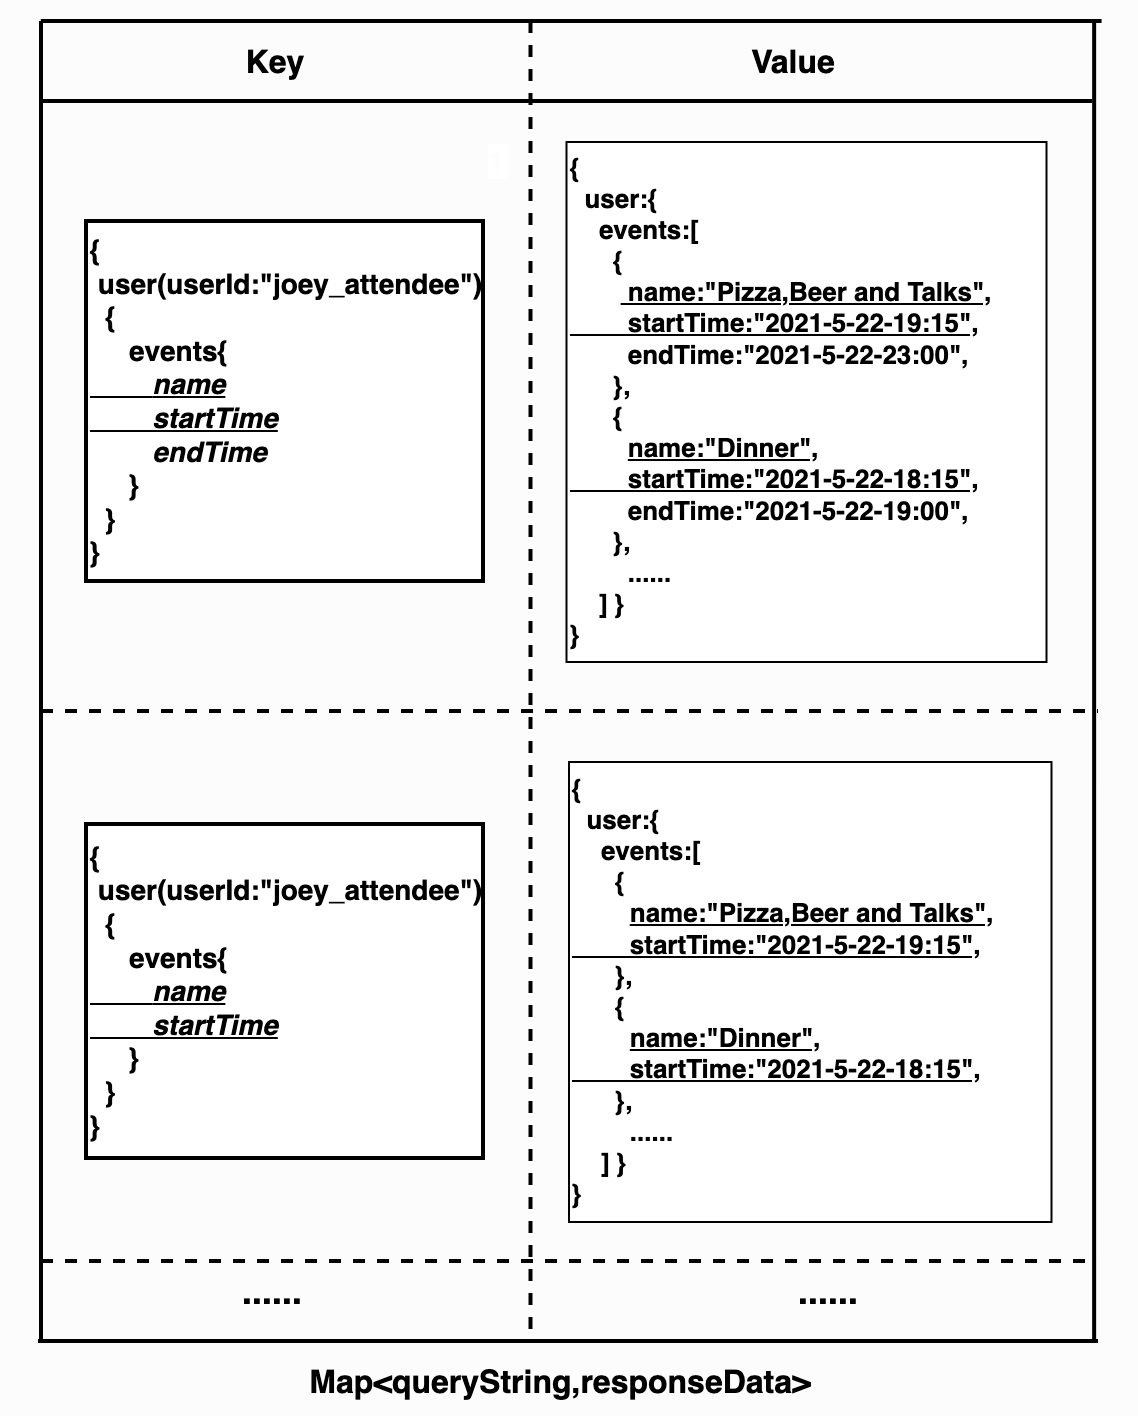
\includegraphics[width=0.8\textwidth]{figure/4-cora/repetitive_cache.png}
	\caption{传统缓存方法在GraphQL场景中的重复缓存问题}
	\label{ontransact-impl}
\end{figure}

具体实现上,基于GraphQL查询语句的特点,Cora考虑了查询语句的嵌套的树形结构,尝试在解析其树形嵌套结构过程中,逐层提取类型和实例数据,并基于遍历完成的节点信息构建查询路径,用全局唯一的查询路径作为缓存的key。此外为了提高缓存命中率,将实例整体而不是查询结果作为缓存的value,这样在一定程度上可以缓解传统缓存方法中的重复缓存问题。举例来说,当用户执行代码4.10所示的查询语句时,
  \begin{lstlisting}[caption={查询语句示例},language=json,basicstyle=\footnotesize] 
    {
        query_airPurifier(_id:"619892261336552"){
            sensor{
                _id
                temp
            }
            speed
        }
    }
   \end{lstlisting}
 Cora会首先会为airPurifier实例构造
 cachePath=\texttt{"/query\_airPurifier(\_id\\:"619892261336552")"},并且为了减少key的大小,Cora用sha256加密算法对cachePath进行加密操作之后,获取前8位“84d889e0”作为缓存key,对应的缓存value是airPurifier实体。Cora会将这条缓存存入AirPurifier对应的CoraNode的缓存槽中。此外,该查询语句中还关联了sensor实例的查询,所以该查询语句中sensor对应的cachePath=\texttt{"query\_airPurifier\\(\_id:"619892261336552")/sensor()"},对应的缓存key为“dfb53ecc9”,对应的缓存value是sensor列表。同样的,Cora会将这条缓存存入Sensor对应的CoraNode的缓存槽中。
 
 当对AirPurifier实例进行更新操作时,Cora会在CoraGraph中获取更新语句相关联的CoraNode    AirPurifier和Sensor,目前框架中采用暴力清空CoraNode缓存的策略,将CoraNode AirPurifier和Sensor中的缓存清空,当然后续可以实现更为先进的缓存更新策略。Cora中使用caffeine作为缓存框架,caffeine\cite{caffeine}是一个高性能的轻量级的java缓存框架,当缓存槽满时,默认采用LRU算法淘汰缓存。
 
综上,Cora中的图缓存模型消除了重复缓存问题,维护了查询语句的结构信息,在确保缓存正确性的前提下提高了缓存命中率。
 
\section{场景构建}
场景构建的核心是支撑场景的运行,并在并发场景运行中,保证场景完整性、有序性和高效性,Cora基于Actor模型构建IoT服务组合场景。根据上文4.1节中的论述,在并发场景处理时,对IoT服务加锁可能会产生死锁问题,而对场景加锁会带来阻塞问题,影响场景高效性,并且使用锁来解决并发问题与上文的事件驱动的IoT服务组合模型并不匹配,而Actor模型可以代替锁来处理并发冲突问题,并且Actor模型可以保证场景高效性,因此Cora基于Actor模型来处理并发场景运行。

场景构建模块主要包括如下模块:

\textbf{状态转移引擎}:状态转移引擎的作用是推动IoT服务根据状态转移模型向前运行。

\textbf{场景消息管理}:场景消息管理的作用是基于场景模型通过推送消息给IoT服务来推动场景运行。

\textbf{场景完整性}:Cora中通过场景确认机制来保证场景完整性。

\textbf{场景有序性}:Cora中通过基于时间戳为场景事件设置场景Id来保证场景有序性。

\textbf{Actor构建}:Cora中,每个Actor都是一个线程,对应于一个IoT服务。

\subsection{状态转移引擎}

状态转移引擎的作用是推动IoT服务根据状态转移模型向前运行,对应于Actor模型中的Internal State处理。本文通过有限状态机模型构建IoT服务的状态转移模型,那么Cora也需要相应的执行引擎来执行有限状态机实例。首先,Cora为每个IoT服务生成enum类型的state字段来描述IoT服务的状态,state字段无需用户用coraML定义,由Cora直接生成,状态转移引擎的主要工作流程就包括解析IoT服务接收的事件,参照CoraNode中的有限状态机模型,获取IoT服务实例当前的state,根据事件信息和state构造GraphQL执行语句,并发送给graphqlEngine处理,更新IoT服务实例的state,推进IoT服务向前运行。具体执行流程如下:
\begin{itemize}
    \item \textbf{事件解析}:
    针对事件,Cora中用coraML定义了事件模型。事件解析器的作用就是按照事先定义的事件格式解析生成Cora中的事件实例,其中包括事件描述,CoraNode类型,IoT服务实例,执行操作等信息,将事件实例提供给执行引擎。
    \item \textbf{状态获取与校验}:
    在执行事件之前,首先需要获取IoT服务实例的当前状态,并根据当前状态和事件实例匹配状态转移模型,判断该IoT服务实例能否匹配事件,更新状态。例如净化器服务在关闭状态时无法接收speed\_up事件,更新状态为high\_speed。所以这一步的目的是校验有限状态机模型,过滤不符合有限状态机模型的事件。具体实现层面,Cora会首先根据事件实例中的CoraNode类型获取相应的状态转移模型,然后根据CoraNode和IoT服务信息生成状态查询语句,发送给graphqlEngine,获取当前IoT服务实例的状态,然后与CoraNode中的状态转移模型进行匹配,获取该IoT服务实例在当前状态下可以接收的事件列表,最后与当前的事件进行匹配,若当前接收事件不在该实例可以接收的事件列表中,不再继续执行,返回相应的错误信息;若当前的事件在该实例可以接收的事件列表中,则继续往下执行,进行GraphQL执行语句的构造。
    \item \textbf{接口构造}:
    根据上文IoT服务生命周期管理的接口生成模块中的阐述,当IoT服务注册在Cora中时,Cora会为IoT服务生成统一标准的操作接口CoraIngress,CoraIngress是更新和查询IoT服务的唯一方式。同样地,在状态转移管理模块中,用户发送事件给Cora时,事件解析器只能解析得到事件实例,需要根据事件实例和当前状态构造GraphQL形式的执行接口,发送给graphqlEngine,这样才能更改IoT服务的状态。具体实现层面,Cora中主要通过定义静态模板,变量替换和语句合成等方式实现,这样的方式在Cora项目中也大量存在。主要有两种场景,一种是构造查询和更新实例数据的接口,因为GraphQL执行语句格式是相对固定的,只有服务实例类型和需要查询的变量会有差异,所以针对很多特定操作,例如查询某个实例的当前状态,更新实例的状态等,可以通过构造静态接口模板的方式将这些执行操作预先定义,这样只要具体执行时进行变量替换便可构造接口实例。代码4.11展示了状态更新模板。
    \begin{lstlisting}[caption={状态更新模板},language=json,basicstyle=\footnotesize]
    updateStateTemplate = 
        {update_${nodeType}(
            _id:\"${id}\",
            data:{
                state:\"${state}\"
            }){
                ${resp}
            }
        }
    \end{lstlisting}
    在变量替换时,为了语句构造和变量校验等必要操作,首先需要获取CoraNode中的变量信息。Cora中用Velocity\cite{velocity}进行变量替换,Velocity是一个高效的基于JVM的模板引擎,使用Velocity可以很方便地进行变量替换操作,当然用java内置的String库也可以完成同样的操作。此外还需要通过语句合成的方式来组合接口,以空气净化器服务为例,调低转速的操作会更新空气净化器服务的转速为low,同时会更新空气净化器服务的状态为低速模式,在这种情况下,基于性能考虑,理想情况下将两条更新操作合并为一条更新操作可以减少一次更新操作,这时候便需要进行语句合成。代码4.12展示了模板语句合成过程。
     \begin{lstlisting}[caption={模板语句合成示例},language=json,basicstyle=\footnotesize] 
     //merge
    updateStateTemplate = 
        {update_airPurifier(
            _id:\"619892261336552\",
            data:{
                state:\"low_speed\"
            }){
                state
            }
        }
    
    updateSpeedTemplate = 
        {update_airPurifier(
            _id:\"619892261336552\",
            data:{
                speed:100
            }){
                speed
            }
        }
    
    updateState&SpeedTemplate = 
        {update_airPurifier(
            _id:\"619892261336552\",
            data:{
                speed:100,
                state:\"low_speed\"
            }){
                speed
                state
            }
        }
    \end{lstlisting}
    可以看到,两条接口语句的data部分和返回变量部分异构,所以需要将data中的更新信息和最后的返回变量进行合并。Cora中用StringBuilder实现,首先定位到两条语句中“data”字段的位置,提取\{\}中的字段进行合并,用相同的方法提取返回变量,完成语句合并过程。
    \item \textbf{接口执行}:
    状态转移引擎中内置了graphqlEngine,将构造好的GraphQL执行语句交由graphqlEngine执行,便可得到相应的执行结果。
\end{itemize}

\subsection{消息管理}
Cora中采用pub/sub模式进行消息处理,Actor完成具体事件的处理,ContextHandler全局监听场景中的事件,并基于IoT服务组合模型负责事件分发,类似于消息中间件中的server端。具体执行流程如下:
\begin{itemize}
    \item \textbf{接收场景事件}:
    用户构建场景完成,向场景发送启动事件,场景解析该事件,并基于场景中的IoT服务字典将该事件推送给对应的IoT服务的mailBox,从而启动整个场景运转。
    \item \textbf{监听Actor执行结果}:
    ContextHandler全局监听场景中Actor的执行结果事件,Actor的执行结果都会publish给ContextHandler,ContextHandler subscribe所有Actor的执行结果事件。
    \item \textbf{事件分发}:
    当接收到某个Actor的执行结果事件时,遍历场景模型的onEvents表,通过匹配id和hook pair寻找符合条件的IoT服务实例,获取其trigger脚本和执行结果,将执行结果填入trigger脚本执行判断,若trigger结果为true,即该场景符合继续推进的场景,则将publishEvent添加到对应的Actor的mailBox中去,完成事件分发过程。注意在定义trigger脚本时,trigger中是一段groovy shell脚本,其判定过程通过Groovy\cite{groovy}实现,Groovy是著名的构建在JVM上的一个轻量级却强大的动态语言,为Java生态提供了很强的动态性,Cora中trigger脚本的判定就是依靠groovy的动态特性实现。
    \item \textbf{场景结束}:
    当ContextHandler接收到执行结果事件,遍历场景模型的onEvents表,无法找到匹配的publishEvent,则场景执行结束。
\end{itemize}

\subsection{场景完整性}
消息不可达或消息丢失可能会影响场景完整性。因为场景完整性要求运行中的场景不能被打断或终止,但是Cora中场景进行消息传递时可能会出现消息不可达或消息丢失的情况,例如\textit{洗衣服场景}中洗衣机服务执行完所有指令后,场景发送给烘干机服务执行指令,烘干机服务可能会丢失消息导致该场景无法继续执行,因此Cora需要保证场景的完整性。

Cora中通过场景确认机制来保证场景完整性。场景确认机制参考RabbitMQ的发送方确认机制(Publisher Confirm)设计实现,当IoT服务执行完场景事件时,需要向场景发送一条反馈事件,场景会一直等待接收反馈事件,若场景接收到反馈事件,则继续往下执行,否则若等待时间大于场景事件运行时间+默认执行延时K(静态设置,远大于执行延时),则向框架抛出场景运行错误事件。

\subsection{场景有序性}
Cora需要保证场景有序性。场景有序性要求在并发场景运行时,需要保证IoT服务执行不同场景的指令之间相对有序。在Cora中,场景有序性受如下两方面影响:1)不同场景执行时发送给同一IoT服务执行指令,而执行指令之间存在相反的运行逻辑。例如当净化器服务在执行完净化器打开指令之后,接收并执行并发场景中净化器关闭指令,最后净化器服务接收到净化器运行指令,但是净化器服务无法在关闭状态下执行运行指令,造成场景执行错误。2)Actor模型的消息传输机制下,Actor异步接收消息会影响场景有序性。例如当用户A和用户B同时执行\textit{洗衣服场景}时,若用户A先运行该场景,则按照场景有序性要求,用户A需要执行完洗衣机服务关闭指令之后,用户B才能运行洗衣机服务,但是基于Actor模型的消息传输机制,洗衣机服务的mailBox中会接收到用户A和用户B的打开洗衣机服务事件,所以用户A的运行洗衣机服务事件将在用户B的打开洗衣机服务事件之后,这会破坏场景有序性。因此Cora需要在框架层保证场景有序性。
\begin{figure}
	\centering
	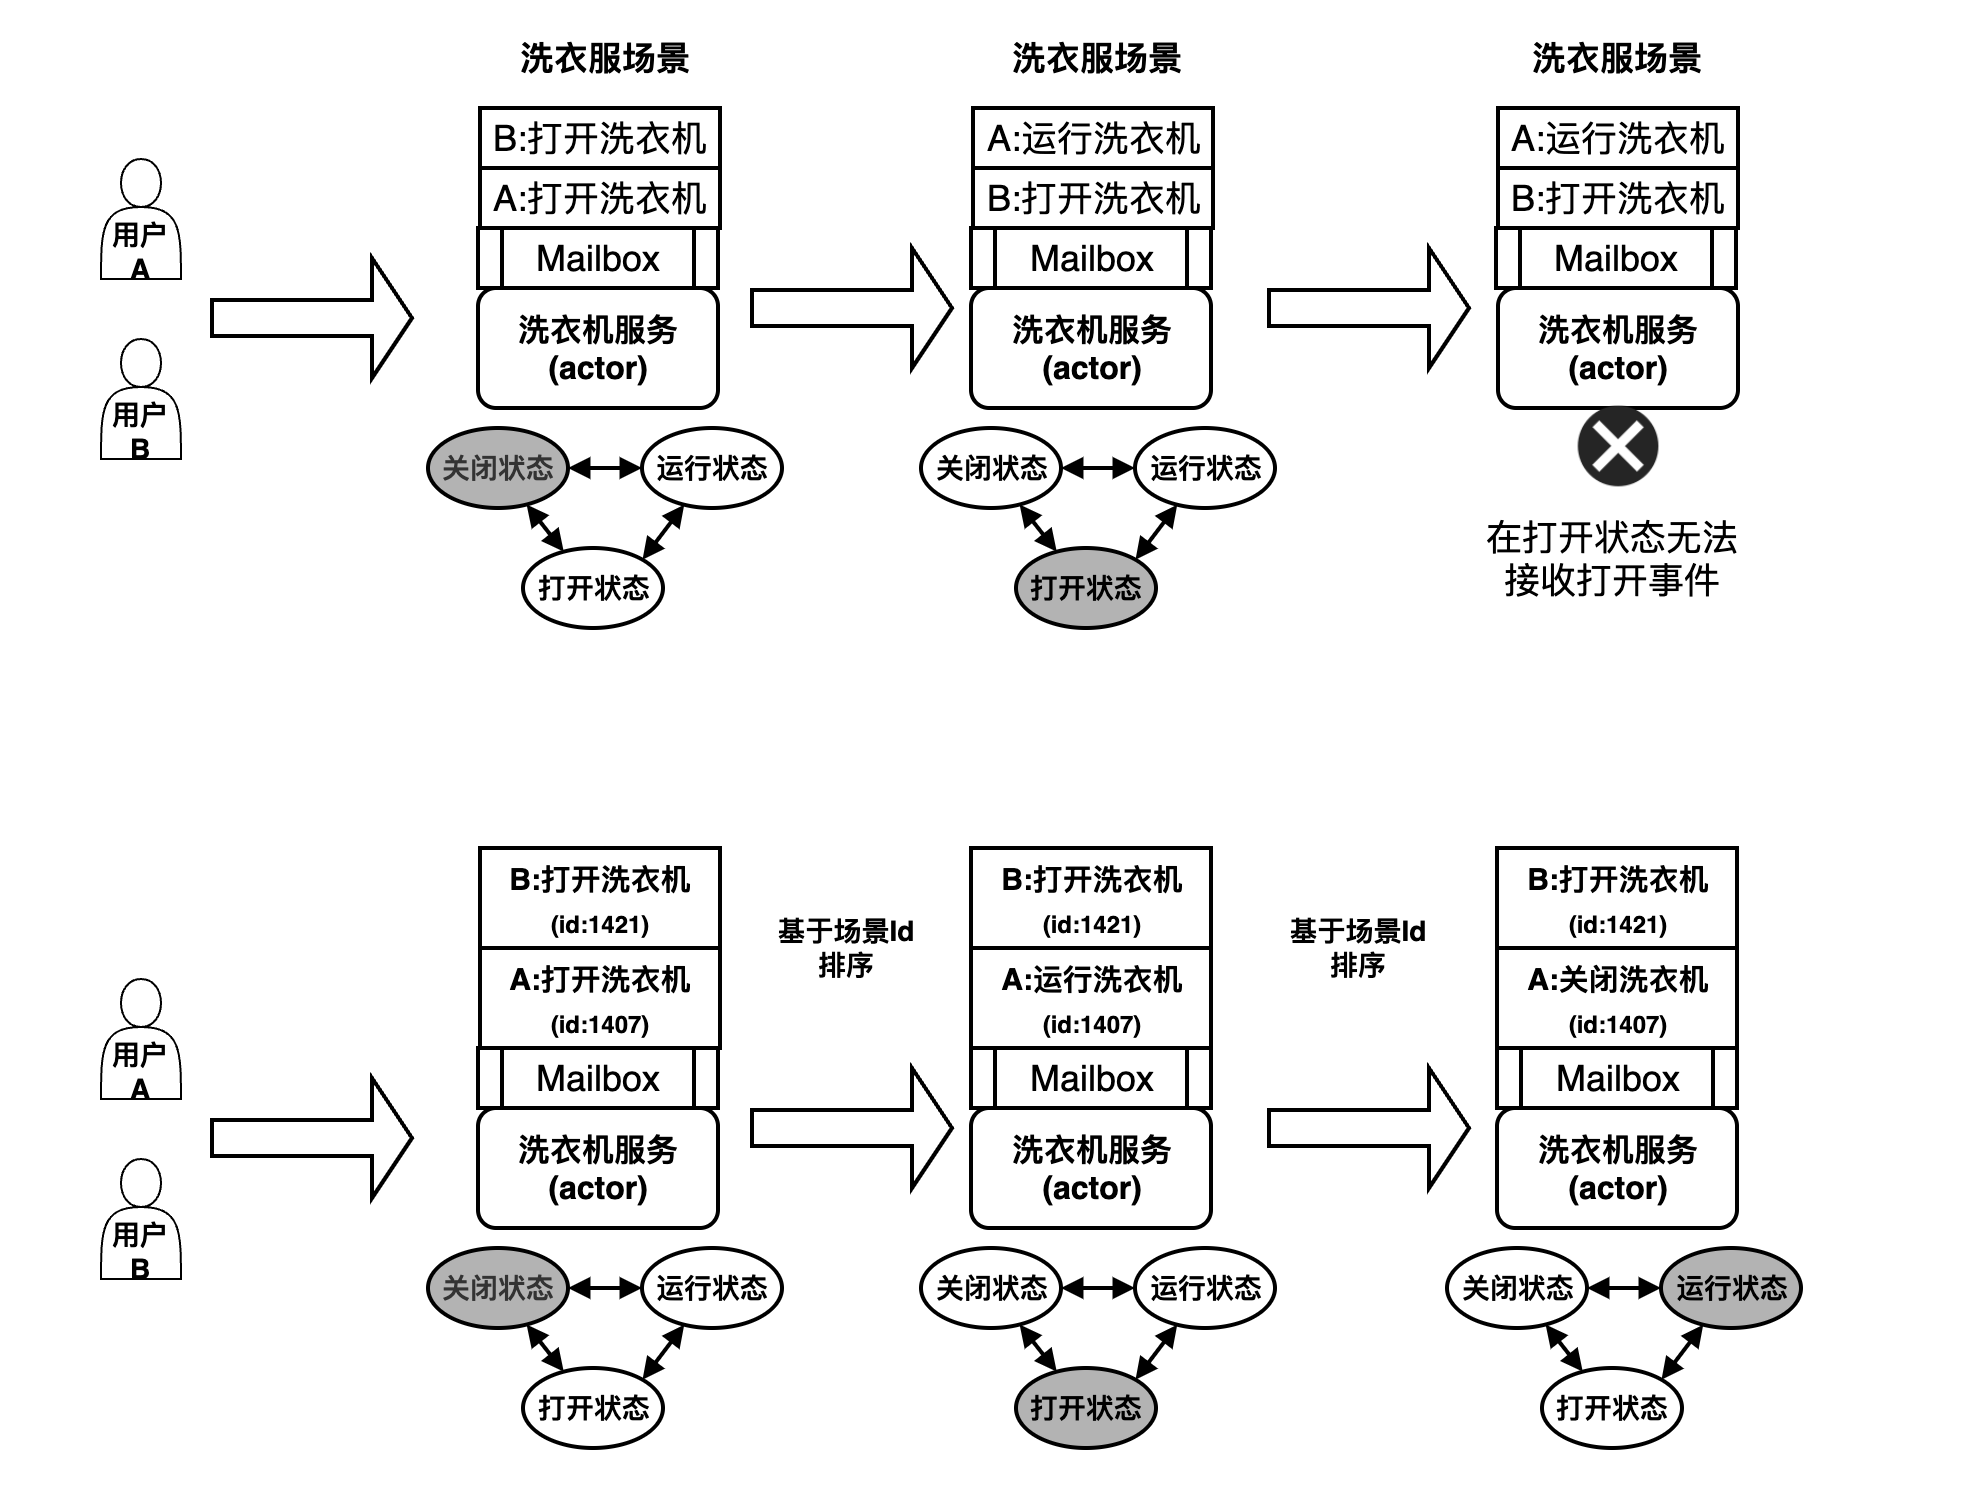
\includegraphics[width=1.0\textwidth]{figure/4-cora/atomicty.png}
	\caption{基于场景Id保证场景有序性}
	\label{ontransact-impl}
\end{figure}

Cora中通过基于时间戳为场景事件设置场景Id来保证场景有序性。当场景开始运行时,Cora会根据当前时间戳为场景生成全局唯一的场景Id,并且场景中的所有事件都会存储该场景Id,当Actor的mailBox接收到事件时,会默认通过场景Id来为mailBox中的事件排序,这样经过排序之后,同一场景中的事件将会连续执行直至该场景中的所有事件执行结束,并且较早执行的场景中的事件会一直处在优先执行的序列,这样便可保证场景的有序性。图5-7展示了Cora基于场景Id保证场景有序性的执行过程,可以看到当洗衣机服务在打开状态时,mailBox中存在用户B的打开洗衣机事件,同时接收到用户Ade运行洗衣机事件,基于场景Id,mailBox会重新对两个事件进行排序,优先执行用户A的运行洗衣机事件,从而保证场景的有序性。


\subsection{Actor构建}
在Cora中,每个Actor都是一个线程,对应于一个IoT服务。代码4.13展示了Actor类型的主要成员变量。
   \begin{lstlisting}[caption={Actor类型结构},label={lst:Actor},language=java,basicstyle=\footnotesize]
    public class ActorImpl extends Thread implements Actor {
        private StateEngine stateEngine;
        
        private EventBus eventBus;
        
        private static final ConcurrentLinkedDeque<Event> mailBox;
        ......
    }
    \end{lstlisting}
    
\begin{itemize}
    \item \textbf{mailBox构建}:
    首先每个Actor都有一个mailBox,mailBox由java中的ConcurrentLinkedDeque实现,队列中存放该Actor接收到的所有事件,在mailBox中基于场景Id来为事件排序,保证场景间的有序性,用户可以自定义消息排序策略。
    \item \textbf{线程构建}:
    其次每个Actor都是一个线程,Actor线程的run()方法会持续监听mailBox,并从中拉取消息,执行消息。
    \item \textbf{消息执行}:
    Actor中有状态转移引擎实例,状态转移引擎实例全局单例,用来具体执行事件。
    \item \textbf{执行结果上报}:
    Actor中还有一个google的EventBus实例,EventBus是一个轻量级的消息总线,允许组件之间通过发布订阅模式相互通信。Actor中的EventBus的作用是,将执行结果以事件的形式发送给场景。
\end{itemize}

\paragraph{冲突处理}
Actor内部的冲突处理主要考虑由于不同场景的作用于同一Actor的矛盾事件的冲突处理问题,这种冲突问题主要集中在命令型事件,在持续型事件中不会出现。例如存在两个场景,运行空调={关闭窗户;打开空调}和关闭空调={打开窗户;关闭空调},当这两个场景的事件是矛盾的,当这两个场景并发执行时,显然会让窗户服务和空调服务不停开关,影响用户体验。本文将这种冲突问题定位到Actor的mailBox中处理,并提供了如下几种处理思路。

\textbf{尽最大努力交付}:即按照Cora的事件处理逻辑运行,不作处理,因为本质上这种问题与运行逻辑无关,只会带来用户体验不足的问题。

\textbf{基于场景优先级}:用户可以自定义场景优先级,当出现冲突情况时,根据场景优先级丢弃场景优先级低的场景。

\textbf{时间片后置}:为场景后置时间片,避免IoT服务的高频调用。

\paragraph{错误处理}
场景执行过程中的错误以日志形式上报。不同于方法调用,Actor模型的错误处理也是异步的。Cora中存在两种可能的错误处理场景。一种是在Actor执行过程中可能会产生错误或异常情况,这种情况与框架无关,Cora会将错误信息封装成事件publish给场景,场景接收到错误事件,以日志形式上报错误信息,用户可以根据日志信息定位到具体Actor。第二种是框架内部错误,这种错误与场景执行无关,是系统内部的错误,这种错误影响较大,同样会以日志形式上报错误信息。

\section{本章小结}
总结来看,本章介绍了基于Actor模型的IoT服务组合框架——Cora。首先对于上章介绍的IoT服务组合模型,本文采用了模型解析的方式解析coraML,并设计实现了CoraGraph管理IoT服务模型;然后基于GraphQL,为IoT服务动态生成了标准统一的生命周期管理接口,并做了查询优化;最后基于Actor模型,完成了IoT服务组合场景的构建。

\chapter{实验评估}

\section{研究问题}
为了评估IoT服务组合建模方法及IoT服务组合框架的有效性,本文基于IoTBench Test Suite中真实的智能家居数据,通过对实验结果的分析来回答如下问题:
\begin{itemize}
	\item 本文提出的IoT服务组合建模方法能否支持真实的IoT服务组合场景构建,Cora能否支持真实的IoT服务组合场景运行?
	\item Cora能否在并发的场景执行中,保证场景的完整性?
	\item 与基于锁实现的相同IoT服务组合场景相比,Cora能否在保证场景完整性的前提下,减少场景阻塞时间?
\end{itemize}

\section{实验配置}
\paragraph{数据集}
本文采用的数据集主要包括两部分:1)Google Home相关用户两年的真实使用数据;2)IoTBench Test Suite:包括35个OpenHAB应用数据\cite{iotbench}。该数据集由SafeHome整理实现。

基于该数据集,本文设计了超过二十种服务组合场景,例如起床场景、洗衣服场景、做早餐场景等。表5-1展示了部分服务组合场景示例,例如起床场景包含三个IoT服务,首先智能灯服务会被唤醒,然后触发闹钟服务,最后智能窗帘会打开。
\begin{table}[!htbp]
	\centering
	\begin{tabular}{cc}
		\toprule
		场景名称 & 场景描述 \\
		\midrule
		起床 & light\_1:on;alarm\_1:on;curtain\_1:open\\
		换衣服 & light\_2:on; curtain\_2:close\\
		洗衣服 & washer:working;washer:off;dryer:working;dryer:off\\
		做早餐 & coffee:on;coffee:off;pancake:on;pancake:off\\
		洗澡 & light\_3:on;door\_1:close;washer:on\\
		打扫房间 & cleanRobot:on;cleanRobot:off\\
		开空调 & window:close;AC:on\\
		\bottomrule
	\end{tabular}
	\caption{部分服务组合场景示例}
	\label{tbl:device_list}
\end{table}
\paragraph{实验设备}
工作站配置如下:
\begin{itemize}
    \item 处理器:2.4 GHz 双核Intel Core i5
    \item 内存:8G
    \item 存储:256G SSD硬盘
    \item 操作系统:MacOS Big Sur
\end{itemize}

\section{实验设计}
\subsection{Cora有效性测试}
Cora的有效性测试主要关注两方面内容:1.本文提出的IoT服务组合建模方法是否能够支持真实的IoT服务组合场景的构建,该建模方法能否减少开发人员的开发负担。2.Cora能够支持真实的IoT服务组合场景的运行,Cora生成的IoT服务的生命周期管理接口能否支持IoT服务的管理。

针对问题1,本文基于真实数据,在Cora中注册足够的IoT服务,并设计实现了二十多中IoT服务组合场景,并通过编码的方式实现其中具有代表性的场景,通过比较两种实现方式的复杂度和代码量,来衡量IoT服务组合建模方法的有效性。针对问题2,本文运行Cora中生成的真实场景,并统计IoT服务的生命周期管理接口的数量来衡量IoT服务组合框架的有效性。

\subsection{并发场景完整性测试}
在并发场景中,场景完整性是IoT服务组合的基础和前提,基于Cora构建的具体的服务组合场景,本文选择具有代表性的真实场景,基于不同的并发负载执行这些场景,通过统计运行中的错误数量来衡量场景完整性。

\subsection{对比SafeHome测试框架执行效率}
根据2.3节,SafeHome被认为是IoT服务组合冲突处理方面的首篇工作,与本文不同,该工作首先定义routine(一系列操控IoT服务的指令列表)具有原子性,并在此前提下,针对并发场景中的冲突问题,SafeHome基于锁机制为开发人员提供了四种可见性模型和相关的冲突处理策略,并在多个实际场景中比较了四种模型的适用性。

SafeHome认为场景具有原子性,并基于该前提定义,提出了并发执行中基于锁的四种可见性模型来保证场景执行安全,实验证明GSV(Global Strict Visibility)模型具有最好的场景安全性,而EV(Eventual Visibility)模型在保证优秀的场景安全性前提下,具有最好的场景高效性。

\textbf{GSV模型}:GSV模型保证全局强原子性,其策略是给场景加锁,场景排队执行,保证同一时间只能有一个场景在执行。GSV模型理论上具有最强的安全性和最差的执行延时。

\textbf{EV模型}:EV模型保证场景的弱原子性,其策略是场景可以在不违背串行顺序的情况下并发执行,给IoT服务加锁,并通过Post/Pre-Lease机制保证场景的安全性。EV模型理论上是锁实现的最优模型,能够在保证场景全局安全性下,提供最好的执行延时表现,SafeHome的实验部分也证明了这一点。

因此本文基于相同场景,分别基于Cora,GSV模型,EV模型运行场景实例,通过比较错误数量和执行延时衡量Cora的执行延时表现。

\section{结果分析}
\subsection{Cora有效性测试结果}

\paragraph{IoT服务组合建模方法}
为了衡量IoT服务组合建模方法的有效性,本文以\textit{净化空气场景}为例,展示开发人员实现该场景的建模过程:

\textbf{构建净化器服务模型和窗户服务模型}:第一步是构建IoT服务模型,\textit{净化空气场景}中有两种IoT服务,所以开发人员需要构建净化器服务和窗户服务这两种IoT服务的设备属性模型及其状态转移模型。图5-1展示了\textit{净化空气场景}中的两种IoT服务模型。
\begin{figure}[H]
	\begin{subfigure}{.5\textwidth}
		\centering
		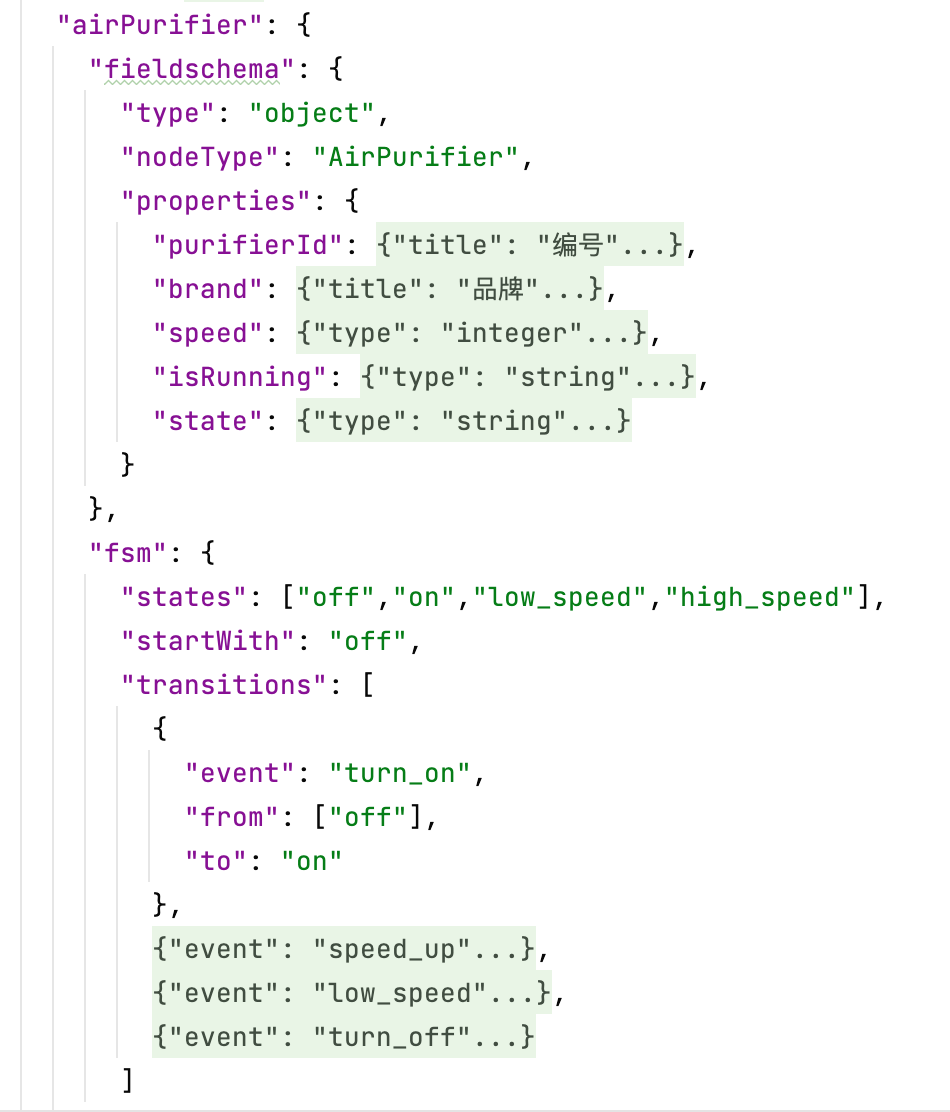
\includegraphics[width=1.0\textwidth]{figure/5-experiment/purifier-model.png}
		\caption{净化器服务模型}
		\label{subfig:a}
	\end{subfigure}
	\begin{subfigure}{.5\textwidth}
		\centering
		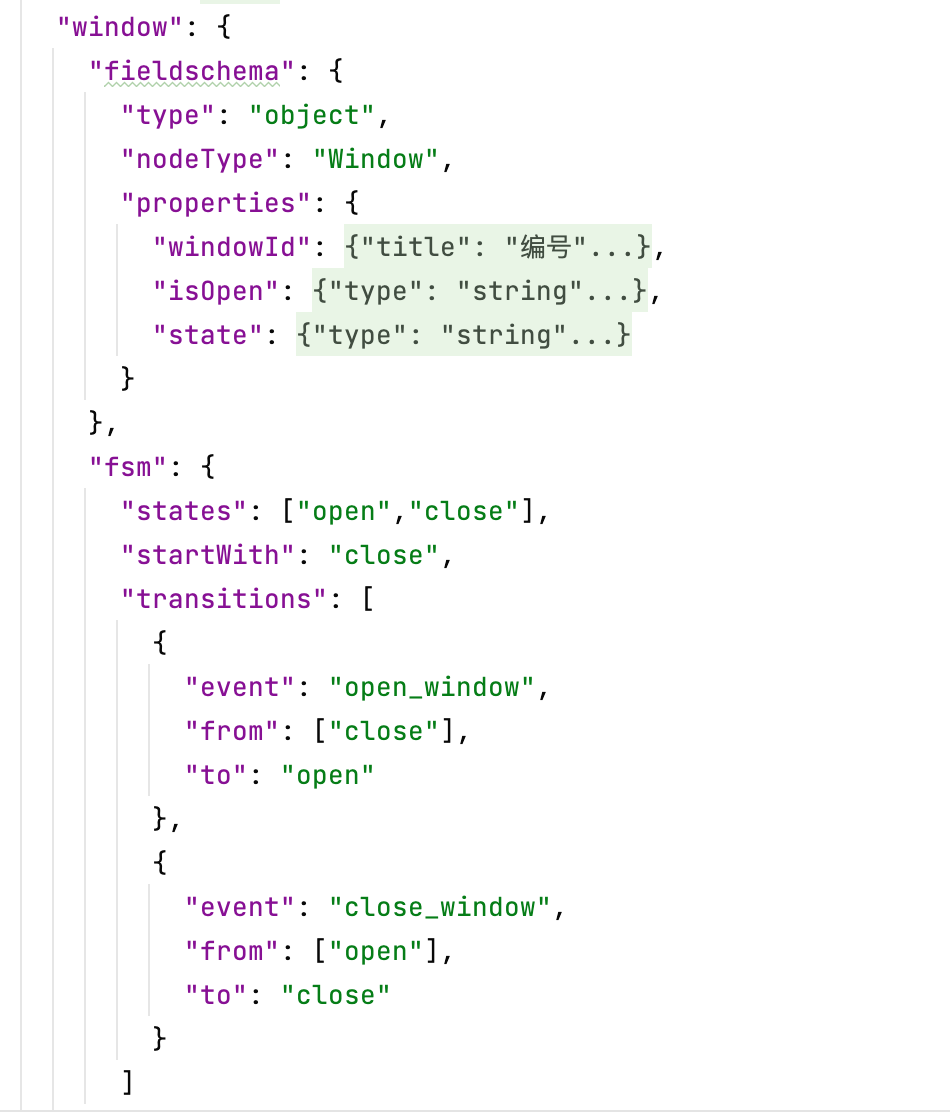
\includegraphics[width=1.0\textwidth]{figure/5-experiment/window-model.png}
		\caption{窗户服务模型}
		\label{subfig:b}
	\end{subfigure}
\caption{净化空气场景中的两种IoT服务模型}
\label{fig:sub}
\end{figure}


\textbf{注册净化器服务和窗户服务实例}:将上述两种服务模型注册到Cora中之后,用户需要注册净化器服务实例和窗户实例到Cora中。图5-2展示了注册净化器服务和窗户服务实例的接口。
\begin{figure}[H]
	\begin{subfigure}{.5\textwidth}
		\centering
		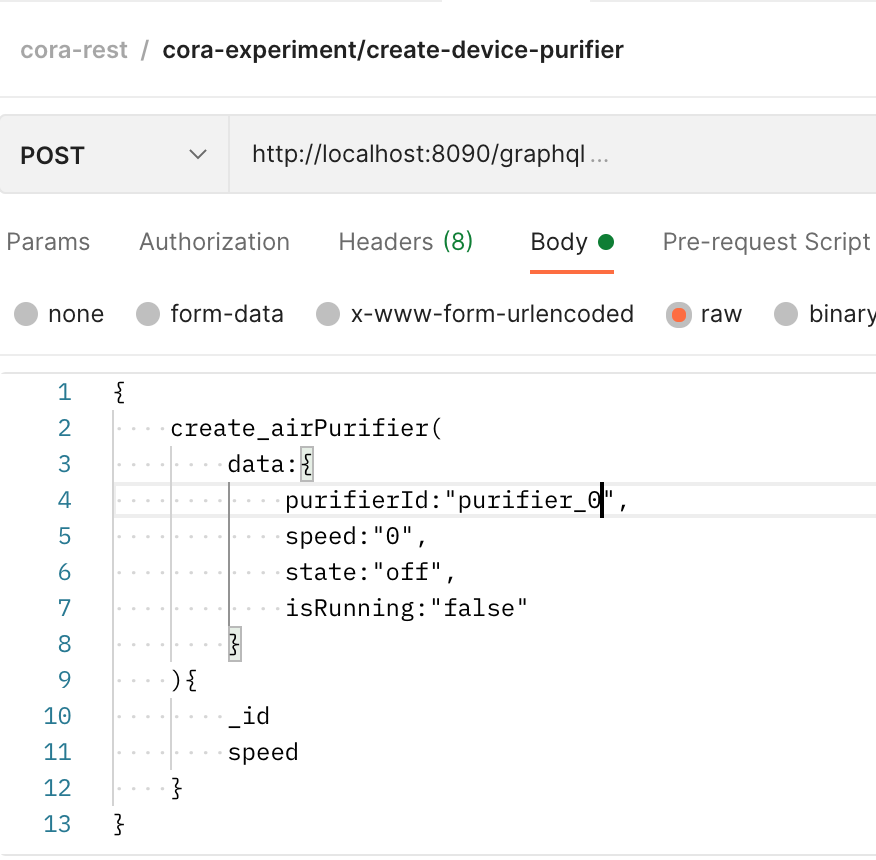
\includegraphics[width=1.1\textwidth]{figure/5-experiment/purifier-api.png}
		\caption{创建净化器服务}
		\label{subfig:a}
	\end{subfigure}
	\begin{subfigure}{.5\textwidth}
		\centering
		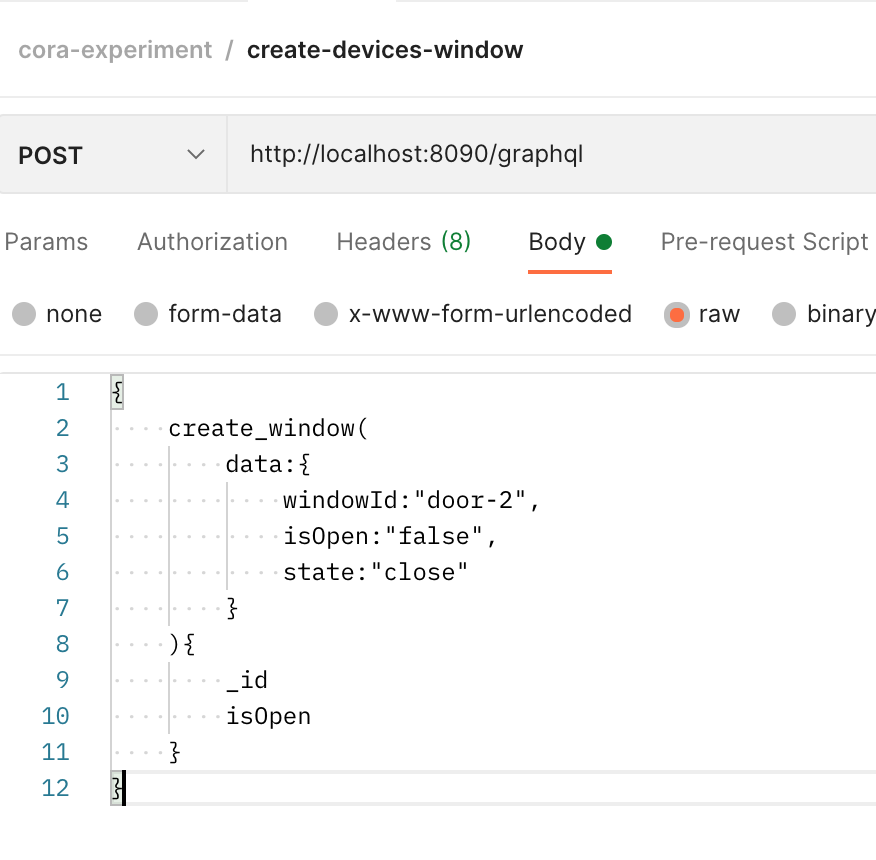
\includegraphics[width=1.1\textwidth]{figure/5-experiment/window-api.png}
		\caption{创景窗户服务}
		\label{subfig:b}
	\end{subfigure}
\caption{注册净化器服务和窗户服务实例}
\label{fig:sub}
\end{figure}

\textbf{构建\textit{净化空气场景}模型}: 在洗衣机服务和烘干机服务注册到Cora中之后,开发人员需要实现场景组合逻辑,即构建\textit{净化空气场景}模型,即在窗户服务运行完成之后,场景需要通知净化器服务运行。图5-3展示了\textit{净化空气场景}模型。
\begin{figure}
	\centering
	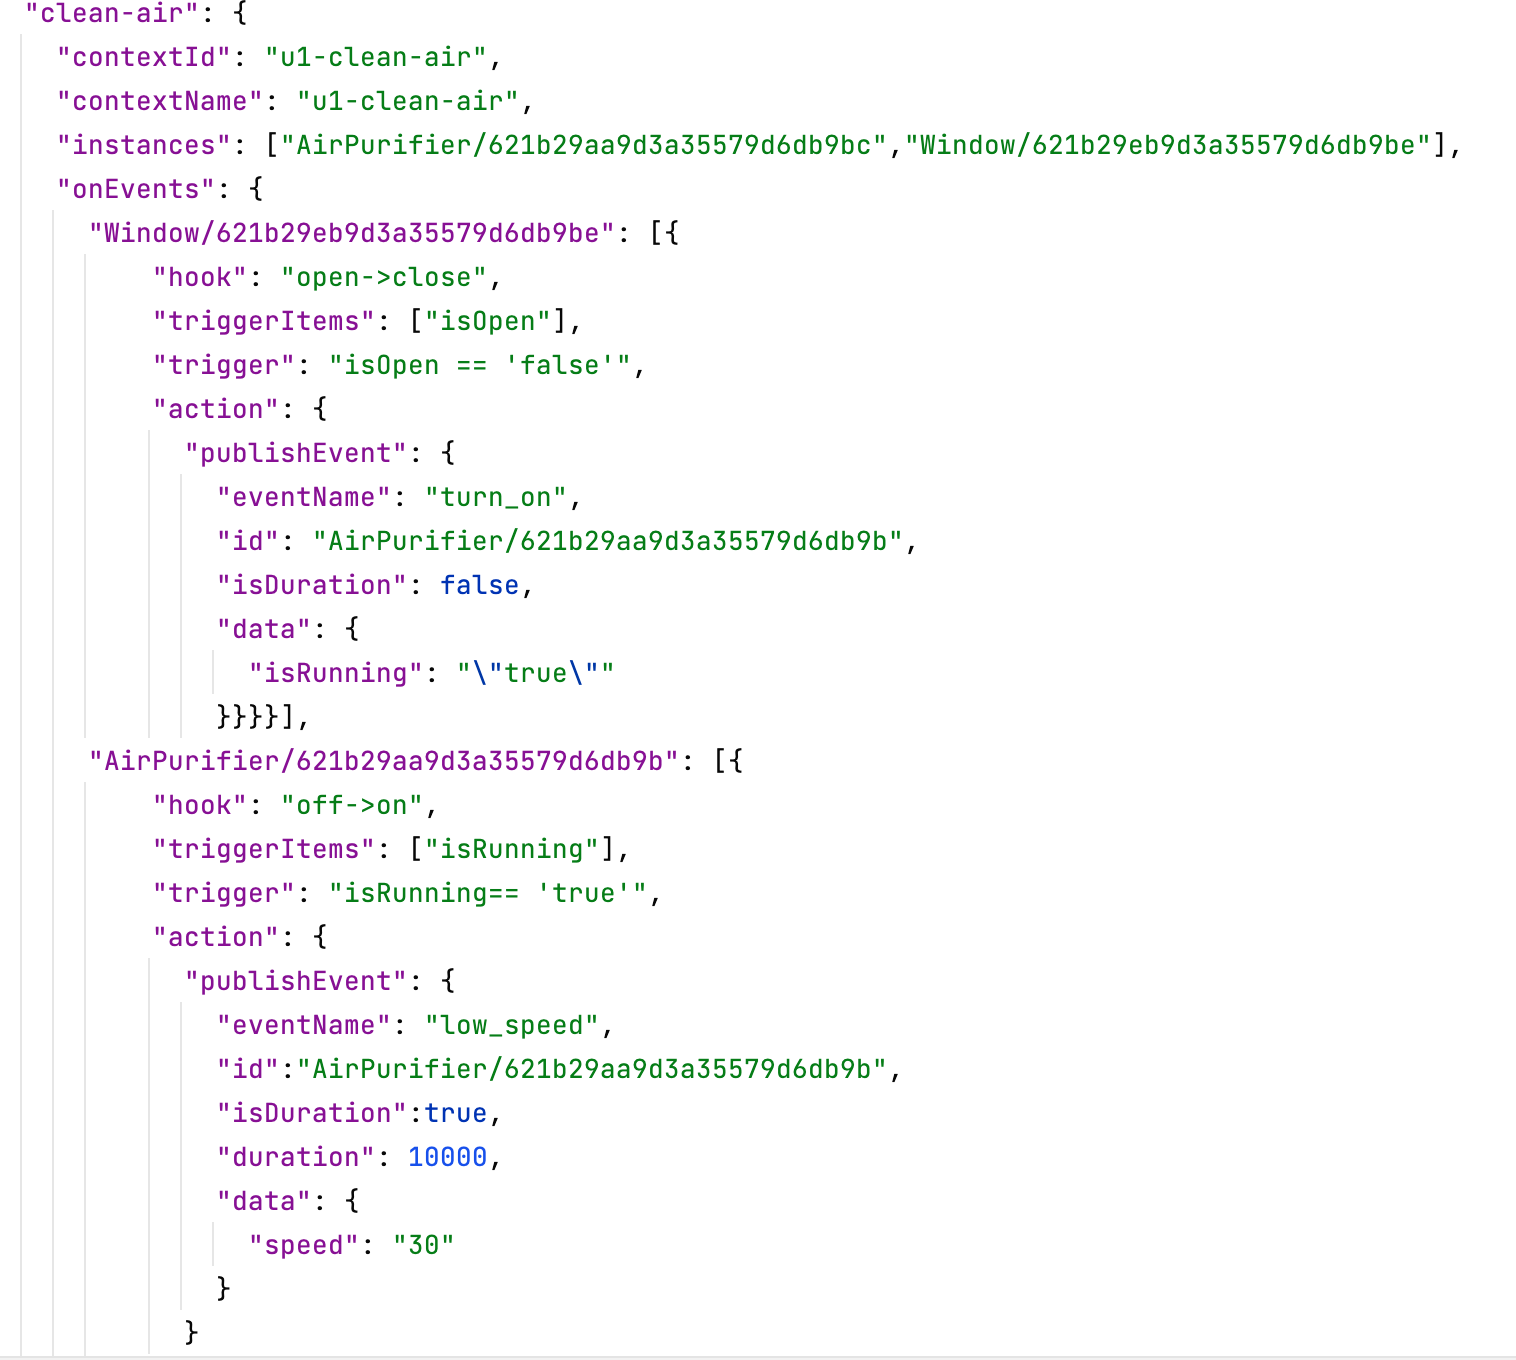
\includegraphics[width=1.0\textwidth]{figure/5-experiment/clean-air-context.png}
	\caption{净化空气场景模型}
	\label{ontransact-impl}
\end{figure}

至此基于IoT服务组合模型构建\textit{净化空气场景}执行完毕,为了衡量本文建模方法的有效性,本文使用Java代码实现\textit{净化空气场景}的流程如下:

\textbf{构建IoT服务模型}:首先定义净化器服务类型和窗户服务类型,定义相关的设备类型属性,并定义方法来描述IoT服务的状态转移逻辑。

\textbf{注册净化器服务和窗户服务实例}:实现数据存储层和接口访问层,代码实现中使用CloudMongodb进行数据存储,基于mongodbRepository来实现数据存储接口,并实现GraphQL接口来管理净化器服务和窗户服务。

\textbf{构建场景}:定义\textit{净化空气场景}逻辑,组合净化器服务的操纵接口和窗户服务的操纵接口。

\begin{table}[!htbp]
\centering
\begin{tabular}{|c|c|c|}
\hline
IoT服务模型 & IoT服务实例注册& 净化空气场景\\
\hline
127 & 265 & 121 \\
\hline
\end{tabular}
\caption{代码实现各模块代码量统计}
\end{table}

实验证明,实现\textit{净化空气场景},本文提出的IoT服务组合建模方法可以减少513行Java代码。

\paragraph{IoT服务组合框架}
本文基于上述数据集,在Cora中注册了12种共计32个IoT服务,并完成了25个IoT服务组合场景构建。起床场景和做早餐场景中服务数量和事件数量较多,且具有代表性,下文将以这两个场景展示实验结果。

首先本文关注Cora为场景中的服务生成的生命周期管理接口的有效性。表5-3是不同场景中生成的IoT服务生命周期管理接口的数量,可以看到生成接口数量与服务数量相关,场景中服务数量越多,生成接口数量也更多。实验证明这些生成接口能够访问IoT服务,接口有效。
\begin{table}[!htbp]
	\centering
	\begin{tabular}{ccc}
		\toprule
		场景描述 & 服务/事件数量  & 生成接口数量 \\
		\midrule
		\{washer:working/20min;washer:off;\\
		dryer:working/15min;dryer:off\} & 2/4 & 14 \\
		\hline
		\{alarm:on/5s;light:on;curtain:open;\\
		tempSensor:on\} & 4/4 & 24  \\
		\hline
		\{coffee:on;coffee:on/10min;coffee:off\\
		microwave:on;microwave:on/5min;microwave:off\\
		toaster:on;toster:on/2min;toaster:off\} & 3/9 & 19 \\
		\hline
		\{light:off;door:off;window:off;AC:off;\\
		curtain:off\} & 5/5 & 29 \\
		\bottomrule
	\end{tabular}
	\caption{场景接口生成结果}
	\label{tbl:device_list}
\end{table}


然后本文测试Cora中的场景实例能否正常运行,并通过实验数据统计场景中事件数量对场景执行延时的影响。表5-4展示了起床场景的执行结果,表5-5展示了做早餐场景的执行结果,实验证明,Cora中的场景实例均能正常执行,没有错误产生。为了保证数据的科学有效性,本文采用执行三次取平均值的策略来进行实验。为了探究场景中事件数量对场景执行延时的影响,在相同IoT服务组成的场景中,本文通过设置不同的事件数量并统计执行延时。根据表5-4,在起床场景中只有1个事件时,执行延时为1.095秒;当起床场景中有闹钟唤醒和打开灯这两个事件时,执行延时为2.256秒;当场景中增加打开窗帘事件时,执行延时为3.788秒;当场景中再增加一个温度传感器读取温度事件时,执行延时为4.252秒。


 因此可以发现,场景的执行延时随着事件数量的增加呈线性增长,每个事件执行的延时在1s左右,执行延迟在可接受范围之内。
\begin{table}[!htbp]
	\centering
	\begin{tabular}{cccc}
		\toprule
		场景描述 & 服务/事件数量  & 执行延时 & 错误数量   \\
		\midrule
		\small\{alarm:on/5s\} & 4/1 & 1.095s & 0  \\
		\hline
	    \small\{alarm:on/5s;light:on\} & 4/2 & 2.256s & 0  \\
		\hline
		\small\{alarm:on/5s;light:on;curtain:open\} & 4/3 & 3.788s & 0  \\
		\hline
		\small\{alarm:on/5s;light:on;curtain:open;\\
		\small tempSensor:on\} & 4/4 & 4.252s & 0  \\
		\bottomrule
	\end{tabular}
	\caption{起床场景执行结果}
	\label{tbl:device_list}
\end{table}

\begin{table}[!htbp]
	\centering
	\begin{tabular}{ccccc}
		\toprule
		场景描述 & 服务/事件数量 & 执行延时 & 错误数量   \\
		\midrule
	    \small\{coffee:on;coffee:on/10min;coffee:off\} & 3/3 & 3.627s & 0  \\
		\hline
		\small\{coffee:on;coffee:on/10min;coffee:off\\
		\small microwave:on;microwave:on/10min;\\
		\small microwave:off\} & 3/6 & 5.495s & 0  \\
		\hline
		\small\{coffee:on;coffee:on/10min;coffee:off\\
		\small microwave:on;microwave:on/5min;\\
		\small microwave:off;toaster:on;toster:on/2min;\\
		\small toaster:off\} & 3/9 & 7.256s & 0  \\
	
		\bottomrule
	\end{tabular}
	\caption{做早餐场景执行结果}
	\label{tbl:device_list}
\end{table}

\subsection{场景完整性测试结果}
表5-6展示了在起床和做早餐场景中,不同并发数量下,场景执行的错误数量均为0。可以证明,在并发场景中场景完整性能够得到保证。
\begin{table}[!htbp]
	\centering
	\begin{tabular}{ccc}
		\toprule
		场景描述 & 服务/事件数量  & 并发错误数量
		        &               &  &     (2/5/10) \\
		\midrule
		\{alarm:on/5s;light:on;curtain:open;\\
		tempSensor:on\} & 4/4 & 0/0/0  \\
		\hline
		\{coffee:on;coffee:on/10min;coffee:off\\
		microwave:on;microwave:on/5min;microwave:off\\
		toaster:on;toster:on/2min;toaster:off\} & 3/9 & 0/0/0 \\
		\bottomrule
	\end{tabular}
	\caption{场景完整性测试结果}
	\label{tbl:device_list}
\end{table}

\subsection{对比测试结果}
图5-4中,图(a)为起床场景的并发测试结果,图(b)为做早餐场景的并发测试结果。该测试基于起床场景及做早餐场景,起床场景=\{alarm:on/5s;light:on;\\curtain:open;tempSensor:on\},该场景由4个IoT服务,共有4个场景事件组成。做早餐场景=\{coffee:on;coffee:on/10min;coffee:off;microwave:on;microwave:on/5min;\\microwave:off;toaster:on;toster:on/2min;toaster:off\},该场景由3个IoT服务,共有9个场景事件组成。


本文分别记录该场景中1到10次并发执行的执行时间和错误数量,在三种模型中,1到10次并发测试均无错误产生。在起床场景的并发测试中,当并发量为1时,三种模型的运行时间都在5.4秒左右;当并发数为2时,GSV模型的运行时间为12.55秒,Cora的运行时间为9.01秒,而EV模型的运行时间为9.56秒;当并发数为5时,GSV模型的运行时间为32.17秒,Cora的运行时间为19.28秒,而EV模型的运行时间为18.38秒;当并发数为10时,GSV模型的运行时间为61.92秒,Cora的运行时间为36.33秒,而EV模型的运行时间为35.21秒。做早餐场景的执行结果可参考图(b)。因此在执行时间对比中,当并发数为1时,因为没有事件阻塞,三种模型执行时间相差不大,而随着并发数量的增加,GSV模型执行时间随并发数量增长线性增长,而基于EV模型实现的系统和Cora的执行时间始终相差不大,且都远小于GSV模型。
  
  
因此可以证明,三种模型在并发场景中都能保证场景的完整性,并且随着并发量的增加,EV模型和Cora的场景阻塞时延相差不大,都远小于EV模型。通过对比测试结果可以看到,Cora在并发测试中能够保证场景完整性,并与SafeHome中基于锁模型实现的最优的EV模型具有相同的场景高效性。
\begin{figure}[H]
	\begin{subfigure}{.5\textwidth}
		\centering
		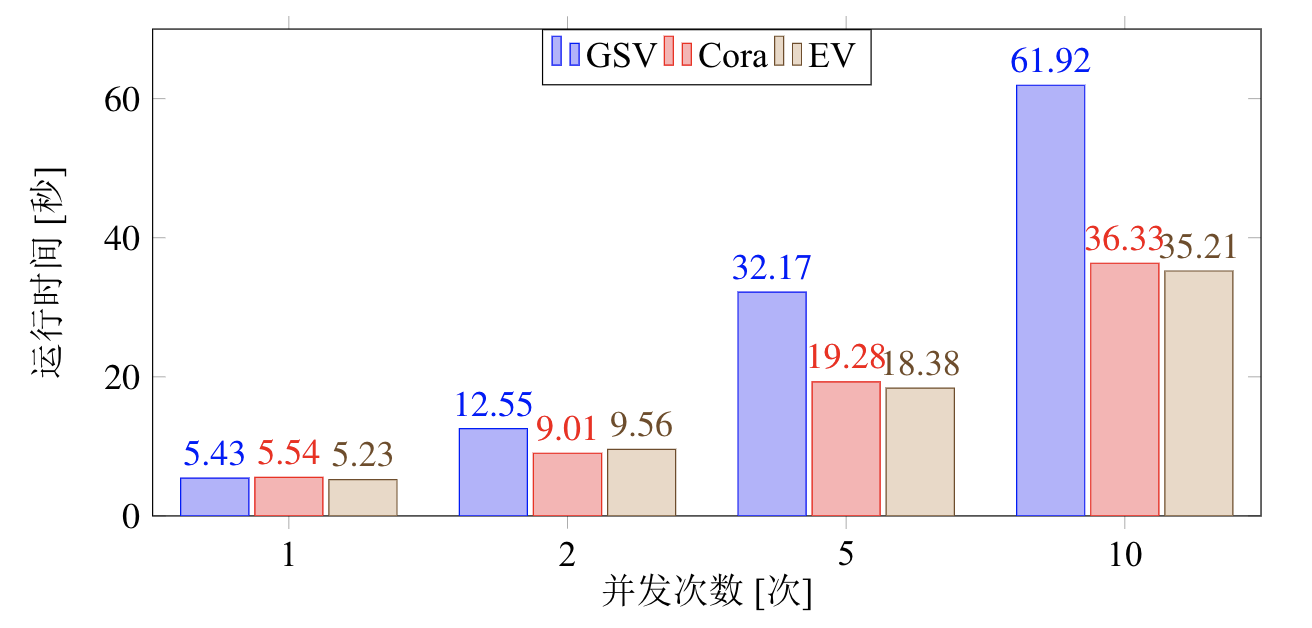
\includegraphics[width=1\textwidth]{figure/5-experiment/concurrency_1.png}
		\caption{起床场景并发测试结果}
		\label{subfig:a}
	\end{subfigure}
	\begin{subfigure}{.5\textwidth}
		\centering
		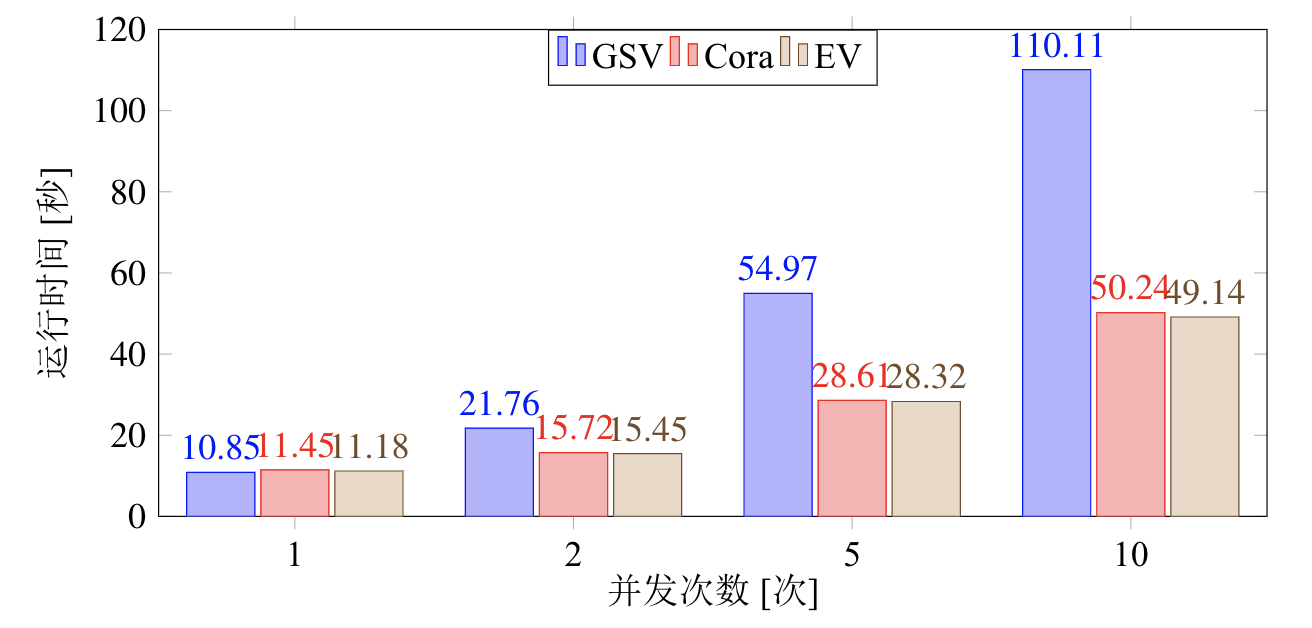
\includegraphics[width=1\textwidth]{figure/5-experiment/concurrency_2.png}
		\caption{做早餐场景并发测试结果}
		\label{subfig:b}
	\end{subfigure}
\caption{并发测试结果}
\label{fig:sub}
\end{figure}

% \pgfplotstableread[row sep=\\,col sep=&]{
%     interval & carT & carD & carR & carA & carB & carC \\
%     1     & 5.432  & 5.535  & 5.229 & 10.847 & 11.454 & 11.184 \\
%     2     & 12.547 & 9.007  & 9.56  & 21.759 & 15.719 & 15.446 \\
%     5    & 32.166 & 19.279 & 18.378 & 54.965 & 28.61 & 28.317 \\
%     10   & 61.92 & 36.332 & 35.214 & 110.112 & 50.238 & 49.141 \\
%     }\mydata
    
% \begin{tikzpicture}
%     \begin{axis}[
%             title={图5-4:起床场景并发执行结果},
%             x tick label style={
%             /pgf/number format/1000 sep=},
%             ybar,
%             bar width=.8cm,
%             width=\textwidth,
%             height=.5\textwidth,
%             legend style={at={(0.5,1)},
%                 anchor=north,legend columns=-1},
%             symbolic x coords={1,2,5,10},
%             xtick=data,
%             nodes near coords,
%             nodes near coords align={vertical},
%             ymin=0,ymax=70,
%             ylabel={运行时间 [秒]},
%             xlabel={并发次数 [次]},
%              enlarge x limits={abs=2*\pgfplotbarwidth}
%         ]
%         \addplot table[x=interval,y=carT]{\mydata};
%         \addplot table[x=interval,y=carD]{\mydata};
%         \addplot table[x=interval,y=carR]{\mydata};
%         \legend{GSV, Cora, EV}
%     \end{axis}
% \end{tikzpicture}
    

% \begin{tikzpicture}
%     \begin{axis}[
%             title={图5-5:做早餐场景并发执行结果},
%             x tick label style={
%             /pgf/number format/1000 sep=},
%             ybar,
%             bar width=.8cm,
%             width=\textwidth,
%             height=.5\textwidth,
%             legend style={at={(0.5,1)},
%                 anchor=north,legend columns=-1},
%             symbolic x coords={1,2,5,10},
%             xtick=data,
%             nodes near coords,
%             nodes near coords align={vertical},
%             ymin=0,ymax=120,
%             ylabel={运行时间 [秒]},
%             xlabel={并发次数 [次]},
%              enlarge x limits={abs=2*\pgfplotbarwidth}
%         ]
%         \addplot table[x=interval,y=carA]{\mydata};
%         \addplot table[x=interval,y=carB]{\mydata};
%         \addplot table[x=interval,y=carC]{\mydata};
%         \legend{GSV, Cora, EV}
%     \end{axis}
% \end{tikzpicture}
\chapter{总结与展望}
\section{工作总结}
本文关注于物联网中的IoT服务组合问题,从IoT服务的特性出发,针对缺乏完善的IoT服务组合建模方法,IoT服务组合场景中的并发冲突等问题,提出了一套模型驱动的IoT服务组合建模方法,降低了开发人员进行IoT服务组合场景开发的工作量;并基于Actor模型实现了一套IoT服务组合框架,在并发执行中保证了场景执行的完整性和有序性,减少了场景阻塞时间,从而提升用户体验。

提出了一套模型驱动的IoT服务组合建模方法及领域特定语言——coraML,本文用coraML为整个场景建模。首先将IoT服务模型分为IoT服务设备属性模型和IoT服务状态转移模型两部分,首先为IoT服务设备属性建模,然后基于有限状态机模型为IoT服务的状态转移逻辑建模;然后针对IoT服务之间的组合逻辑,用消息驱动的方式为场景建模,并用事件模型驱动IoT服务内部向前运转以及场景的运转。

设计实现了一个基于Actor模型的IoT服务组合框架——Cora。本文基于Actor模型的设计理念,将Cora分为三个模块,首先是模型管理模块,针对IoT服务组合模型,Cora设计了相应的模型解析器,并用实体关系模型CoraGraph统一管理IoT服务模型;然后Cora基于CoraGraph注册IoT服务,并为IoT服务生成标准统一的GraphQL风格的接口,并针对GraphQL的N+1问题,用查询语句过滤和图缓存优化的方式优化查询接口;最后完成场景构建,设计状态转移引擎来支撑IoT服务的状态转移,基于EventBus实现场景消息管理,并基于Actor模型,在保证场景完整性的前提下,框架提供了最优的场景阻塞时间。

经试验分析证实,在智能家居场景下,Cora能够支持复杂的IoT服务组合场景的构建,在并发场景中能够保证场景执行的完整性,并且在与基于锁模型实现的相同场景的对比中,表现出了最好的场景阻塞时延。
\section{研究展望}
我们下一步的研究内容可能包括以下方面:

\textbf{基于IoT服务时空属性的调度策略:}Cora主要考虑了智能家居场景下的服务组合问题,IoT服务的时空属性并不明显,默认采用一种预先指定的调度策略。当考虑更大的物联网场景,例如智慧快递,智慧城市等,IoT服务的时空属性就会对IoT服务组合产生很大的影响,例如智能快递下的路线规划问题主要考虑快递车的位置属性。所以基于IoT服务时空属性的调度策略是本文未来的一个研究方向。

\textbf{更多考虑用户体验:}用户体验是IoT服务组合技术最需考虑的问题,Cora能够解决程序意义上的冲突问题,但是对于一些指令事件组成的场景,例如开空调场景=\{关闭窗户;打开空调\},当用户A想要打开空调,而用户B有相反想法时,就会造成用户体验上的冲突问题;此外目前用户仍然需要通过模型定义的方式来构建场景,如何让用户无感知地运行场景,例如框架可以自动为用户构建一些常用场景,当传感器感知到用户行为或空间变化时可以自动触发这些场景。这些问题是本文后续需要关注的问题。



%%%%%%%%%%%%%%%%%%%%%%%%%%%%%%%%%%%%%%%%%%%%%%%%%%%%%%%%%%%%%%%%%%%%%%%%%%%%%%%
% 致谢,应放在《结论》之后


\begin{acknowledgement}
三年的硕士生涯即将过去,回望过去,最大的感受是充实和忙碌,三年的求学时光收获满满,给我留下了很多深刻美好的回忆。在学位论文即将完成之际,我要在此向所有给我提供帮助和支持的人表达最诚挚的感谢。

我要感谢我的导师曹春老师,感谢他提供给我一个继续读研的机会,让我能够在南京大学计算机系继续攻读我的硕士学位,也是曹老师将我领进了软件工程的大门,培养了我的工程素养和软工思维。进入软件所以来,曹老师给我提供了大量宝贵的工程实践机会,也在项目实践和日常交流中提供给我很多指导和教诲,他兢兢业业的工作态度和精益求精的钻研精神深深影响了我,让我受益匪浅。本文从选题、系统设计、成文到修改都离不开曹老师的耐心指导。

感谢南京大学计算机系的各位老师,从本科到硕士,是你们的课程和教学引我走进了计算机科学的大门,帮助我掌握了扎实的专业技能。感谢软件所各位老师和同学对我的关心和帮助,让我的研究生生活更加充实。

感谢王东宇、廖祥森师兄对我微服务研究领域的引导,感谢韩沅锡、陈哲霏、王国畅同学在项目实践中的帮助,还要感谢王国畅同学在我论文撰写过程中给我提供的各种帮助。感谢实验室的各位师兄和我的室友段建辉、韩沅锡同学平日的照顾和陪伴。

感谢我的父母、家人、陈越和挚友们,在外求学不易,是你们一如既往的支持和鼓励帮助我排忧解难,让我能够顺利度过遇到的困难和挫折。

最后要感谢南京大学,在南京大学学习的七年时光是我人生中最美好的回忆,在南京大学120周年校庆之际,祝愿南京大学越来越好。
\end{acknowledgement}


%%%%%%%%%%%%%%%%%%%%%%%%%%%%%%%%%%%%%%%%%%%%%%%%%%%%%%%%%%%%%%%%%%%%%%%%%%%%%%%




% 参考文献。应放在\backmatter之前。
% 推荐使用BibTeX,若不使用BibTeX时注释掉下面一句。
%\nocite{*}
\bibliography{sample}


% 附录,必须放在参考文献后,backmatter前

%%%%%%%%%%%%%%%%%%%%%%%%%%%%%%%%%%%%%%%%%%%%%%%%%%%%%%%%%%%%%%%%%%%%%%%%%%%%%%%
% 书籍附件
\backmatter
%%%%%%%%%%%%%%%%%%%%%%%%%%%%%%%%%%%%%%%%%%%%%%%%%%%%%%%%%%%%%%%%%%%%%%%%%%%%%%%
% 作者简历与科研成果页,应放在backmatter之后

\begin{resume}
% 论文作者身份简介,一句话即可。
\begin{authorinfo}
\noindent 汤聪,男,汉族,1997年11月出生,江苏常州人。
\end{authorinfo}
% 论文作者教育经历列表,按日期从近到远排列,不包括将要申请的学位。
\begin{education}
\item[2019年9月 --- 2022年6月] 南京大学计算机科学与技术系 \hfill 工学硕士
\item[2015年9月 --- 2019年6月] 南京大学计算机科学与技术系 \hfill 理学学士
\end{education}
% 论文作者在攻读学位期间所发表的文章的列表,按发表日期从近到远排列。
\begin{publications}
\item 发明专利:一种基于图模型的GraphQL查询开销优化方法(专利号:202210530499.1)
\end{publications}
% 论文作者在攻读学位期间参与的科研课题的列表,按照日期从近到远排列。
\begin{projects}
\item 国家重点研发计划:软件定义的人机物融合云计算支撑技术与平台(2018YFB1004805),2018年5月—2021年4月,负责云计算支撑平台的设计与实现。
\end{projects}
\end{resume}

%%%%%%%%%%%%%%%%%%%%%%%%%%%%%%%%%%%%%%%%%%%%%%%%%%%%%%%%%%%%%%%%%%%%%%%%%%%%%%%
% 生成《学位论文出版授权书》页面,应放在最后一页
\makelicense

%%%%%%%%%%%%%%%%%%%%%%%%%%%%%%%%%%%%%%%%%%%%%%%%%%%%%%%%%%%%%%%%%%%%%%%%%%%%%%%
\end{document}
